%%
%% This is file `sample-acmsmall.tex',
%% generated with the docstrip utility.
%%
\documentclass[acmsmall,screen,review]{acmart}
%\documentclass[acmsmall,screen,review,anonymous,nonacm]{acmart}
%%
%% \BibTeX command to typeset BibTeX logo in the docs
\AtBeginDocument{%
  \providecommand\BibTeX{{%
    \normalfont B\kern-0.5em{\scshape i\kern-0.25em b}\kern-0.8em\TeX}}}

\setcopyright{acmcopyright}
\copyrightyear{2026}
\acmYear{2026}
\acmDOI{XXXXXXX.XXXXXXX}

%% These commands are specific to PACMPL (for OOPSLA Round 2)
\acmJournal{PACMPL}
\acmVolume{1}
\acmNumber{PLDI}
\acmArticle{1}
\acmMonth{1}


%% Packages
\usepackage{multirow}
\usepackage{booktabs} % For formal tables
\usepackage{stmaryrd}
\usepackage{adjustbox}
\usepackage{subcaption}
\usepackage[ruled,vlined,linesnumbered]{algorithm2e}
\usepackage{algpseudocode}
\usepackage{subcaption}
\usepackage{rotating}
\usepackage{xcolor}
% TikZ and Quantikz
\usepackage{tikz}
\usetikzlibrary{quantikz2}
\usetikzlibrary{shapes.geometric, arrows, arrows.meta, positioning}

% Comment commands


\usepackage{wrapfig}
\usepackage{graphicx}

\newcommand{\showcomment}[1]{#1}
\newcommand{\yfc}[1]{\showcomment{\textcolor{blue}{\textbf{YFC:} #1}}}
\newcommand{\bw}[1]{\showcomment{\textcolor{green}{\textbf{BW:} #1}}}
\newcommand{\cy}[1]{\showcomment{\textcolor{blue}{\textbf{CY:} #1}}}
\newcommand{\rmark}[1]{\textcolor{red}{#1}}
\newcommand{\bmark}[1]{\textcolor{blue}{#1}}


%\renewcommand{\yfc}[1]{}
% \renewcommand{\bw}[1]{}
\renewcommand{\cy}[1]{}


\newcommand{\cC}{\mathcal{C}}
\newcommand{\cD}{\mathcal{D}}
\newcommand{\cE}{\mathcal{E}}
\newcommand{\cF}{\mathcal{F}}
\newcommand{\cS}{\mathcal{S}}
\newcommand{\cL}{\mathcal{L}}





\citestyle{acmauthoryear}

\begin{document}

\title{Formal Verification of  Flagged Fault-Tolerant Error Correction Protocols}

\author{Bo-Ruei Wu}
\affiliation{%
  \institution{Academia Sinica}
  \city{Taipei}
  \country{Taiwan}
}

\author{Yu-Fang Chen}
\affiliation{%
  \institution{Academia Sinica}
  \city{Taipei}
  \country{Taiwan}
}

\author{Ching-Yi Lai}
\affiliation{%
  \institution{National Yang Ming Chiao Tung University}
  \city{Hsinchu}
  \country{Taiwan}
}

% \begin{abstract}
% Fault-tolerant syndrome extraction protocols using flag qubits can reduce the number of required ancilla qubits or circuit rounds, making them attractive for near-term fault-tolerant quantum computing architectures. However, the design and validation of such circuits typically rely on intricate manual analysis of error propagation patterns. Ensuring that all possible fault combinations are properly accounted for can be challenging. Subtle issues in gate ordering, ancilla interactions, or measurement scheduling may lead to unintended error propagation, resulting in correlated data errors and, in the worst case, logical failures.

% In this work, we propose a SAT-based formal verification framework for \emph{flagged error correction protocols}. We focus on a central correctness property: for any set of up to $t = \lfloor (d-1)/2 \rfloor$ circuit-level faults, the resulting data errors must either be non-degenerate or yield distinguishable syndrome and flag outcomes. We encode Pauli fault propagation, measurement behavior, and bounded-fault constraints as Boolean formulas, and verify correctness by proving the unsatisfiability of configurations that violate this property.
 
% Using our framework, we analyze several representative flagged circuits and identify design flaws that violate the specified correctness property. Our results demonstrate that SAT-based formal verification provides a rigorous and systematic approach to validating fault-tolerant quantum circuit constructions.
% \end{abstract}

\begin{abstract}
\yfc{Please check whether the characterization in the abstract and conclusion
states the protocol-validity assumptions explicitly.}
% Fault-tolerant syndrome extraction protocols based on flag qubits provide a
% resource-efficient approach to quantum error correction, but their correctness
% is difficult to verify. Such protocols combine syndrome-extraction circuits with classical control and recovery. Therefore, verification must check not only the
% circuits themselves, but also whether the measurement record along each
% execution path contains enough information for fault-tolerant recovery.


% In this work, we show that explicit decoder construction is unnecessary for verifying flagged error correction protocols. We prove that a fault-tolerant decoder exists if and only if all fault events consistent with the same measured record produce correctable errors . This result enables the verification of decoder existence without constructing the decoder itself.

% This paper develops a formal verification method for flagged fault-tolerant
% error-correction protocols. Instead of fixing a particular lookup-table decoder,
% we give a decoder-independent criterion for whether the measurement records
% produced by the protocol are sufficient for fault-tolerant recovery. For a valid
% protocol, this criterion requires that, for every measurement record, all
% residual Pauli errors consistent with that record are jointly correctable:
% equivalently, no two such residual errors differ by a nontrivial logical
% operator.

% Based on this characterization, we develop a formal verification framework that symbolically models Pauli fault propagation, measurement outcomes, and protocol control flow. We encode violations of the distinguishability property as satisfiability queries and automatically search for counterexamples using SAT solving.
% We implement our method and evaluate it on a large collection of representative protocols from the literature, successfully validating known constructions while identifying subtle counterexamples in optimized designs. Notably, these findings include design flaws in parallel syndrome extraction for the $[[5,1,3]]$ code, low-depth protocols for the $[[7,1,3]]$ code, and flag-condition violations in higher-distance protocols.




Fault-tolerant syndrome extraction with flag qubits provides a resource-efficient approach to quantum error correction by using measurement outcomes to adapt the subsequent error-correction procedure. This adaptive control flow, however, makes correctness difficult to verify: to guarantee correction of a specified set of faults, any two non-equivalent faults must be distinguishable by the resulting execution paths and measurement records, since they may require incompatible recoveries. 
In this work, we establish a criterion for verifying a fault-tolerant lookup-table decoder without explicitly constructing the table: a valid decoder exists if and only if all residual errors consistent with each measurement record are jointly correctable. 
We develop a formal verification framework that symbolically tracks Pauli faults, measurement outcomes, and adaptive control flow, and uses SAT solving to search for violations of this condition. 
We evaluate the framework on representative flagged protocols from the literature, successfully validating known constructions and exposing errors in previously published protocols.


\end{abstract}




%\cy{don't say Liou and Bhatnagar; cite their papers in the manuscript}

\begin{CCSXML}
<ccs2012>
   <concept>
       <concept_id>10010583.10010786.10010813</concept_id>
       <concept_desc>Hardware~Quantum error correction and fault tolerance</concept_desc>
       <concept_significance>500</concept_significance>
   </concept>
   <concept>
       <concept_id>10003752.10003790.10003794</concept_id>
       <concept_desc>Theory of computation~Automated reasoning</concept_desc>
       <concept_significance>500</concept_significance>
   </concept>
 </ccs2012>
\end{CCSXML}

%\ccsdesc[500]{Hardware~Quantum error correction and fault tolerance}
%\ccsdesc[500]{Theory of computation~Automated reasoning}

%\keywords{Fault tolerant quantum computing, Verification, SAT}

\maketitle

%\bw{change ST solver}
\section{Introduction}
\yfc{To reduce the main text to 20 pages, merge the first two background
paragraphs into one. In the characterization paragraph, keep the formal
criterion and one sentence explaining incompatible recoveries; remove
the repeated explanations beginning ``Equivalently'' and ``When this condition holds''.}

Quantum error correction is essential for realizing reliable quantum
computation on noisy physical devices~\cite{Shor96}. Quantum error-correcting
codes (QECCs) encode logical information into multiple physical qubits and
provide protection against physical faults~\cite{CS96,Ste96}. 
% For a code ofdistance $d$, ideal error correction can correct any Pauli error of weight at most $t=\lfloor(d-1)/2\rfloor$. 
In practice, however, the error-correction
circuitry is itself imperfect, and faults during syndrome extraction can
propagate into high-weight data errors and cause logical failures.


Fault-tolerant error correction (FTEC) addresses this problem by designing
syndrome extraction and recovery procedures that remain reliable in the
presence of circuit faults~\cite{Shor96,AGP06,CDT09:CCS:2011814.2011815}.
Early approaches by Shor~\cite{Shor96}, Steane~\cite{Steane97}, and Knill~\cite{Knill05}
use carefully prepared ancillary states and verification circuits, but can
incur substantial resource overhead.
Flagged fault-tolerant error correction
provides an alternative based on a small number of additional ancilla qubits,
called \emph{flag qubits}~\cite{Chao18,CR18b}, and has since been extended to
higher-distance codes and improved through parallelization, flag sharing, and
adaptive low-depth control flow~\cite{Chamberland18,reichardt2021fault,LL23,Liou25,Du24,low-depth}.



% \emph{Flagged fault-tolerant error correction protocols}~\cite{Chao18,CR18b} provide an alternative approach to fault-tolerant error correction using a small number of additional qubits. Instead of using large verified ancilla states, these protocols introduce simple ancilla qubits, called \emph{flag qubits}, into syndrome extraction circuits. When an internal fault may propagate to a high-weight data error, the flag measurement outcome provides  information that enables the \emph{decoder} to select an appropriate recovery operation. The original flagged scheme was introduced by Chao and Reichardt~\cite{Chao18} for distance-3 codes and was later extended to higher-distance stabilizer codes by Chamberland and Beverland~\cite{Chamberland18}. Subsequent work has further improved flagged protocols through parallelization, flag sharing, and adaptive low-depth control flow~\cite{reichardt2021fault,LL23,Liou25,Du24,low-depth}.
% Despite their resource advantages, flagged protocols are challenging to design and verify. 
% A flagged fault-tolerant error correction protocol must ensure that any two correctable fault events are either distinguishable from the measurement outcomes or produce equivalent residual errors on the data qubits.
% Otherwise, the decoder may fail to identify a recovery operation that correctly handles both cases. Establishing this property requires careful coordination of gate ordering, qubit reuse, measurement scheduling, classical control flow, and the decoding procedure.

Despite their resource advantages, flagged protocols are challenging to
design and verify. Their performance depends on the detailed structure of
the syndrome extraction circuits and the adaptive control flow, including
gate ordering, qubit reuse, measurement scheduling, and the choice of
subsequent syndrome extraction circuits based on previous measurement
outcomes. Different fault events may produce the same measurement record,
so the measurement record may not contain sufficient information to determine
a valid recovery.

In this paper, we develop a systematic framework for the verification of
flagged fault-tolerant error correction protocols. We focus on whether the
information generated by a protocol is sufficient to support a fault-tolerant
recovery. Here, a \emph{measurement record} consists of the syndrome and flag
outcomes collected along an adaptive execution path. For a fixed terminating
path and measurement record, multiple residual Pauli errors may be compatible
with the observed outcomes. The central question is whether a single recovery
can correctly handle all such residual errors.


% % A flagged protocol must be checked not only for Pauli fault propagation
% % through its syndrome extraction circuits, but also for whether its
% % \emph{measurement record} contains sufficient information for fault-tolerant
% % recovery. For a fixed terminating path and measurement record, multiple
% % residual Pauli errors may be compatible with the observed outcomes. The key
% % question is whether these residual errors can be handled by a common recovery.

% % This observation exposes the central verification problem addressed in this paper. 
% A flagged protocol must be checked not only for Pauli fault propagation
% through its syndrome extraction circuits, but also for whether its \emph{measurement
% record} contains sufficient information for fault-tolerant recovery. 
% % Themeasurement record consists of the \emph{syndrome and flag outcomes} collected along an adaptive execution path. 




A decoder-dependent verification approach would first construct a lookup-table
decoder and then check whether the resulting correction satisfies the
fault-tolerant error-correction conditions for every fault event within the
fault bound. This is not the most informative verification target. If such a
check fails, the failure may arise either from the choice of decoder or from the
protocol itself: the syndrome and flag outcomes may simply fail to distinguish
fault events that require different recoveries. We therefore formulate the
verification condition directly in terms of the residual-error sets associated
with measurement records, rather than a preselected decoder.


Our main characterization shows that, for a valid flagged fault-tolerant error
correction protocol, FTEC is achieved if and only if no two residual errors
associated with the same measurement record differ by a
\emph{nontrivial logical operator}~\cite{KL97,Got97}.
Equivalently, any two fault events within the fault bound that follow the same
terminating path and produce the same measurement record must leave residual
data errors that can be handled by a common recovery.
When this condition holds, a single recovery can be assigned to each measurement record to correctly handle
all compatible residual errors. When it fails, the same measurement record is
compatible with two logically inequivalent residual errors, and no recovery
depending only on that record can correctly handle both cases.


Based on this characterization, we develop a SAT-based verification framework.
We formulate the syndrome extraction circuits and fault events as SAT
constraints and search for pairs of fault events that produce the same
measurement record but leave residual errors whose product is a nontrivial
logical operator. A satisfying assignment provides an explicit counterexample
to FTEC, while the absence of such an assignment establishes that a suitable
lookup-table decoder exists. 
The framework symbolically propagates Pauli faults
through syndrome extraction circuits, computes syndrome and flag outcomes
along adaptive execution paths, and derives the corresponding residual data
errors. The resulting constraints
capture both the circuit-level fault propagation and the adaptive control flow,
allowing the verifier to search systematically over all fault events within
the fault bound.



We implement the method and evaluate it on representative flagged protocols from the literature. The evaluation demonstrates two uses of the verifier. First, it validates known
constructions by proving that their concrete formal instantiations satisfy the
required validity and FTEC conditions. Second, it exposes errors that are
difficult to detect by manual inspection. During benchmark construction, the
verifier repeatedly caught concrete instantiation mistakes while translating
protocol descriptions into executable formal models. More substantively, it
identified previously unnoticed flaws in optimized protocols from the
literature, including counterexamples in low-depth protocols for the
$[[5,1,3]]$ and $[[7,1,3]]$ codes and flag-condition violations in
higher-distance protocols. These issues were reported to the corresponding
authors and confirmed. Together, these results show that automated verification
is useful not only for checking new protocol designs, but also for ensuring that
published protocols are faithfully instantiated and for detecting subtle
correctness bugs in the protocols themselves.





\section{Preliminaries}
This section introduces the notation and conventions used throughout the paper. 
We first review the binary representation of Pauli operators and the fundamental notions of stabilizer codes, including syndromes, degeneracy, and logical equivalence.
%In particular, we establish a formal criterion for verifying whether a syndrome extraction circuit correctly implements the intended stabilizer measurements. The criterion requires that, after measurement, the measurement qubits are disentangled from the data block, and that the fault-free circuit produces measurement outcomes consistent with the eigenvalues of the measured stabilizers.
 Finally, we define the symbolic Pauli propagation semantics and the circuit-level fault model used by our verifier.



\subsection{Pauli operators and binary representation}
\label{subsec:pauli-binary}

We consider the Pauli operators $I$, $X$, $Y$, and $Z$ modulo
global phases in $\{\pm1,\pm i\}$, which do not affect
syndromes, measurement outcomes, or logical equivalence.
We use the standard binary representation~\cite{NC00}:
\begin{equation}
I\mapsto(0,0),\quad X\mapsto(1,0),\quad
Z\mapsto(0,1),\quad Y\mapsto(1,1).
\end{equation}

An $n$-qubit \emph{Pauli string}
$P=P_1\otimes\cdots\otimes P_n$ is represented by
\begin{equation}
P=(P_{1,x},P_{1,z},\ldots,P_{n,x},P_{n,z}),
\label{eq:binary}
\end{equation}
where $(P_{i,x},P_{i,z})$ denotes the binary representation
of $P_i$. We use the same notation for a Pauli operator
and its binary representation when clear from context.
Pauli multiplication, denoted by $\cdot$, corresponds
to bitwise XOR modulo global phase:
\begin{equation}
P\cdot Q=P\oplus Q.
\label{eq:pauli_prod}
\end{equation}
The \emph{weight} $\mathrm{wt}(P)$ is the number of
non-identity components of $P$.

The commutation relation between two Pauli strings
$P$ and $Q$ is determined by their binary symplectic
product:
\begin{equation}
P\odot Q=
\bigoplus_{j=1}^{n}
\left(
(P_{j,x}\land Q_{j,z})
\oplus
(P_{j,z}\land Q_{j,x})
\right).
\label{eq:symp_ip}
\end{equation}
Here, $\oplus$ and $\land$ denote Boolean XOR and AND.
The operators commute if $P\odot Q=0$ and
anti-commute otherwise; equivalently,
$P\cdot Q=(-1)^{P\odot Q}Q\cdot P$.


\subsection{Stabilizer codes, syndromes, and degeneracy}
\label{subsec:stablizer-syndromes-degeneracy}

An $[[n,k,d]]$ \emph{stabilizer code} encodes $k$ logical
qubits into $n$ physical qubits with distance $d$~\cite{Got97}.
It is defined by $n-k$ independent, mutually commuting
Pauli generators $G_1,\ldots,G_{n-k}$, which generate the
stabilizer group
$\mathcal{S}=\langle G_1,\ldots,G_{n-k}\rangle$.
The code space is their common $+1$ eigenspace.
The logical Pauli operators
$\mathcal{L}=\{\bar X_1,\ldots,\bar X_k,
\bar Z_1,\ldots,\bar Z_k\}$
generate the logical Pauli group modulo $\mathcal{S}$.

Two Pauli errors $E_1$ and $E_2$ are
\emph{stabilizer-equivalent}, written $E_1\sim E_2$,
if $E_1\cdot E_2\in\mathcal{S}$ up to global phase.
Such errors act identically on encoded states.
The minimum weight of an error up to stabilizers is
\begin{equation}
\mathrm{wt}_{\mathrm{min}}(P)
=\min_{S\in\mathcal{S}}\mathrm{wt}(P\cdot S).
\label{eq:wt_min}
\end{equation}

The \emph{syndrome} of a Pauli error $E$ is
\begin{equation}
\mathrm{syn}(E)
=(E\odot G_1,\ldots,E\odot G_{n-k}),
\label{eq:syndrome}
\end{equation}
where $\odot$ is the binary symplectic product.
The syndrome map is linear:
$\mathrm{syn}(E\cdot F)
=\mathrm{syn}(E)\oplus\mathrm{syn}(F)$.

The \emph{normalizer} $N(\mathcal{S})$ consists of
Pauli operators commuting with every stabilizer.
Its elements have zero syndrome, while
$N(\mathcal{S})\setminus\mathcal{S}$ consists of
nontrivial logical Pauli operators.
The code distance $d$ is the minimum weight of
an operator in $N(\mathcal{S})\setminus\mathcal{S}$.
A set $\mathcal{E}$ of Pauli errors is
\emph{correctable} if and only if~\cite{KL97,Got97}
\begin{equation}
\forall E_1,E_2\in\mathcal{E},\quad
E_1^\dagger\cdot E_2
\notin N(\mathcal{S})\setminus\mathcal{S}.
\label{eq:QECC_condition}
\end{equation}
Here, $E^\dagger=E$ up to global phase.

Consequently, any two errors of weight at most
$t=\lfloor(d-1)/2\rfloor$ with the same syndrome
are stabilizer-equivalent.
An \emph{ideal decoder} performs fault-free syndrome
extraction and applies a corresponding correction,
thereby correcting any error with
$\mathrm{wt}_{\mathrm{min}}(E)\le t$.





\subsection{Symbolic Pauli propagation}

We symbolically track Pauli errors using a pair of Boolean
formulas $(Q_{i,x},Q_{i,z})$ for each qubit $i$, allowing
the verifier to analyze fault configurations without
enumerating them or simulating quantum states.

We consider Clifford circuits with ancillas initialized
in $\ket{0}$ or $\ket{+}$ and measured in the $X$ or $Z$
basis. Since Clifford gates preserve Pauli operators
under conjugation, error propagation can be represented
by Boolean updates. Figure~\ref{fig:two-qubit-pauli-rules}
shows the CX and CZ propagation rules used by our verifier.
For a qubit with symbolic error $(Q_{i,x},Q_{i,z})$,
a $Z$-basis measurement yields the error-induced outcome
bit $Q_{i,x}$, while an $X$-basis measurement yields
$Q_{i,z}$.




\begin{figure}[t]
\centering

\begin{subfigure}{0.48\linewidth}
\centering
\begin{quantikz}[row sep={1.2cm,between origins}, column sep=0.6cm]
\lstick{$(Q_{cx}, Q_{cz})$} & \ctrl{1} & \qw
  \rstick{$(Q_{cx}, Q_{cz} \oplus Q_{tz})$} \\
\lstick{$(Q_{tx}, Q_{tz})$} & \targ{} & \qw
  \rstick{$(Q_{tx} \oplus Q_{cx}, Q_{tz})$}
\end{quantikz}
\caption{CX gate}
\end{subfigure}
\hfill
\begin{subfigure}{0.48\linewidth}
\centering
\begin{quantikz}[row sep={1.2cm,between origins}, column sep=0.6cm]
\lstick{$(Q_{cx}, Q_{cz})$} & \ctrl{1} & \qw
  \rstick{$(Q_{cx}, Q_{cz} \oplus Q_{tx})$} \\
\lstick{$(Q_{tx}, Q_{tz})$} & \control{} & \qw
  \rstick{$(Q_{tx},  Q_{tz} \oplus Q_{cx})$}
\end{quantikz}
\caption{CZ gate}
\end{subfigure}

\vspace{0.8em}

\caption{Symbolic Pauli propagation through CX and CZ gates.
Each pair $(Q_x,Q_z)$ represents the Pauli error
on the corresponding qubit.}
\label{fig:two-qubit-pauli-rules}



\end{figure}




We consider Clifford circuits with ancillas initialized in
\yfc{Delete this paragraph and the following measurement-outcome paragraph:
both repeat the explanation immediately before the CX/CZ figure.
Keep the earlier explanation and the figure.}
$\ket{0}$ or $\ket{+}$ and measured in the $X$ or $Z$
basis. Since Clifford gates map Pauli errors to Pauli
errors, their propagation can be tracked symbolically
using the binary representation.
Figure~\ref{fig:two-qubit-pauli-rules} illustrates the
CX and CZ propagation rules used by our verifier.

For a symbolic Pauli error $(Q_{i,x},Q_{i,z})$,
a $Z$-basis measurement produces an error-induced
outcome flip $Q_{i,x}$, while an $X$-basis measurement
produces a flip $Q_{i,z}$.





\subsection{Circuit-level noise model}
\label{sec:circuit-level-noise-model}

We use a circuit-level Pauli fault model, in which a
\emph{fault} at a circuit location is represented by a
Pauli error inserted after the corresponding ideal
operation. For a single-qubit location, a fault applies
a non-identity Pauli operator from $\{X,Y,Z\}$. For a
two-qubit location acting on qubits $i$ and $j$, a fault
applies a nontrivial two-qubit Pauli error
$P_i\otimes P_j$, where $P_i,P_j\in\{I,X,Y,Z\}$ and
$(P_i,P_j)\neq (I,I)$.

Preparation, measurement, and idle faults are modeled
similarly: a preparation fault inserts a Pauli error
immediately after state preparation, a measurement fault
inserts a Pauli error immediately before measurement,
and an idle fault inserts a non-identity single-qubit
Pauli error on the idle qubit.

\section{Fault-tolerant error correction and flagged syndrome extraction}\label{sec:flagged-SE}
This section introduces our formal framework for flagged error correction protocols and FTEC. We start by formalizing basic unflagged syndrome extraction circuits, which we then extend to define the full flagged error correction protocol, including its underlying circuits and classical control flow. After formally defining protocol validity, we establish the necessary and sufficient conditions for a valid protocol to achieve FTEC.



\subsection{Syndrome extraction circuits}
\label{subsec:syndrome extraction-protocols}

A \emph{syndrome extraction circuit} couples data qubits
to ancillas initialized in $\ket{0}$ or $\ket{+}$ and
measures them to extract stabilizer syndromes.
Multiple extraction circuits may execute in parallel,
provided their correctness and measurement determinism
are preserved.

\begin{definition}
\label{def:syndrome-extraction-correct}
A Clifford syndrome extraction circuit $U$ for Pauli
checks $\{P_i\}_{i=1}^{m}\subseteq\mathcal{S}_{\mathrm{data}}$
is \emph{correct} if, for every input data Pauli error $E$,
the propagated error
\[
U(E\otimes I_{\mathrm{anc}})U^\dagger
=\omega(E'\otimes E_{\mathrm{anc}})
\]
satisfies
\[
E_{\mathrm{anc}}\odot A_i=E\odot P_i
\quad(i=1,\ldots,m),\qquad E'\sim E,
\]
where $A_i$ is the designated ancilla measurement
observable and $\omega$ is a global Pauli phase.
\end{definition}

Correctness ensures that ancilla error propagation
reproduces the intended syndrome parities while
preserving data errors up to stabilizer equivalence.
It does not guarantee deterministic measurements.

\begin{definition}
\label{def:syndrome-extraction-deterministic}
A syndrome extraction circuit is \emph{deterministic}
if, in the absence of circuit faults, every input
data Pauli error determines all ancilla measurement
outcomes independently of the encoded state, and
the output data remains in the codespace up to
a Pauli error. For an error-free input, all ancilla
outcomes are $+1$, and the encoded logical state
is preserved up to global phase.
\end{definition}

\begin{definition}
\label{def:syndrome-extraction-valid}
A syndrome extraction circuit is \emph{valid}
if it is both correct
(Def.~\ref{def:syndrome-extraction-correct})
and deterministic
(Def.~\ref{def:syndrome-extraction-deterministic}).
\end{definition}

The following theorem characterizes validity using
stabilizer and logical-operator preservation, enabling
an efficient check via stabilizer simulation.

\begin{theorem}
\label{thm:syndrome-extraction-valid}
Let $U$ be a Clifford syndrome extraction circuit
before ancilla measurements, with
\[
\mathcal{S}_{\mathrm{joint}}
=\langle G_1,\ldots,G_{n-k},A_1,\ldots,A_r\rangle,
\]
where $G_i$ are data stabilizer generators and
$A_i$ are the single-qubit ancilla preparation
and measurement observables. Among the $r$ ancillas,
the first $m$ extract the designated Pauli checks
$\{P_i\}_{i=1}^{m}\subseteq\mathcal{S}_{\mathrm{data}}$.
Let $L_1,\ldots,L_{2k}$ be Hermitian representatives
of a complete set of logical Pauli generators,
extended by identities on the ancillas.

Then $U$ is valid if and only if it is correct and
\[
\begin{gathered}
U\mathcal{S}_{\mathrm{joint}}U^\dagger
=\mathcal{S}_{\mathrm{joint}},\\
(UL_iU^\dagger)L_i\in\mathcal{S}_{\mathrm{joint}}
\qquad(i=1,\ldots,2k).
\end{gathered}
\]
Both stabilizer equality and membership retain
Pauli signs.
\end{theorem}

The proof is given in Appendix~\ref{app:proof-syndrome-extraction}.

Figure~\ref{fig:three-part-syndrome-bad} illustrates
an invalid parallel syndrome extraction circuit
from~\cite{KL24}. Although the individual circuits
extract $XX$ and $ZZ$ correctly, their parallel
execution entangles the ancillas, making the
measurement outcomes nondeterministic.
Thus, circuit validity cannot be inferred from
the validity of individual extraction circuits.

The \emph{ideal syndrome} of a data error $E$
with respect to a Pauli check $P$ is $E\odot P$,
whereas the \emph{measured syndrome} consists of
the actual ancilla measurement outcomes.
A \emph{full syndrome extraction round} measures
a generating set of data stabilizers.
For a valid fault-free round, the measured syndrome
equals $\mathrm{syn}(E)$.

\begin{figure}[h]
    \centering
    
    % --- Top Left: Subfigure A (Isolated XX) ---
    \begin{subfigure}{0.29\linewidth}
        \centering
        \scalebox{0.85}{
        \begin{quantikz}[row sep=0.4cm, column sep=0.4cm]
            \lstick{$Q_1$}              & \targ{}   & \qw     & \qw \\
            \lstick{$Q_2$}              & \qw       & \targ{}  & \qw \\
            \lstick{$Q_{anc}$ \ket{+}}  & \ctrl{-2} & \ctrl{-1}& \meter{X}
        \end{quantikz}}
        \caption{$X_1X_2$ Syndrome Extraction}
        \label{fig:iso-x}
    \end{subfigure}
    \hfill
    % --- Top Right: Subfigure B (Isolated ZZ) ---
    \begin{subfigure}{0.29\linewidth}
        \centering
        \scalebox{0.85}{
        \begin{quantikz}[row sep=0.4cm, column sep=0.4cm]
            \lstick{$Q_1$}              & \qw & \ctrl{2} & \qw      & \qw       & \qw \\
            \lstick{$Q_2$}              & \qw & \qw      & \ctrl{1} & \qw       & \qw \\
            \lstick{$Q_{anc}$ \ket{0}}  & \qw & \targ{}  & \targ{}  & \meter{Z} & \qw
        \end{quantikz}}
        \caption{$Z_1Z_2$ Syndrome Extraction}
        \label{fig:iso-z}
    \end{subfigure}
    \hfill
    \begin{subfigure}{0.39\linewidth}
        \centering
        \scalebox{0.85}{
        \begin{quantikz}[row sep=0.4cm, column sep=0.5cm]
            \lstick{$Q_1$}               & \targ{}   & \qw      & \qw       & \ctrl{3} & \qw      \\
            \lstick{$Q_2$}               & \qw       & \ctrl{2} & \targ{}   & \qw      & \qw      \\
            \lstick{$Q_{anc1}$ \ket{+}}  & \ctrl{-2} & \qw      & \ctrl{-1} & \qw      & \meter{X}  \\
            \lstick{$Q_{anc2}$ \ket{0}}  & \qw       & \targ{}  & \qw       & \targ{}     & \meter{Z}
        \end{quantikz}}
        \caption{Parallel Syndrome Extraction }
        \label{fig:combined-bad}
    \end{subfigure}
    
  \caption{An example of syndrome extraction for a stabilizer state with
$\mathcal{S}=\langle XX,ZZ\rangle$.
(a) and (b) show the individual syndrome extraction circuits for $XX$ and
$ZZ$, respectively. (c) A parallel syndrome extraction circuit for $XX$ and
$ZZ$, which is invalid because the measurement outcomes are not deterministic.}
    \label{fig:three-part-syndrome-bad}
\end{figure}


\subsection{Equivalent circuit-level noise model}

For verification purposes, we consider only the possible Pauli errors induced by faults in the circuit and do not consider their rates or probabilities.  Therefore, we have the following proposition to reduce the complexity for verification. 
We assume that every data qubit participates in at least one CNOT or CZ
gate during syndrome extraction.


\begin{proposition}
\label{prop}
For the purpose of enumerating possible Pauli error patterns in Clifford syndrome extraction circuits, it is sufficient to introduce fault variables only at two-qubit gate locations. Input data errors and faults occurring at state preparation, measurement, idle, and single-qubit gate locations can be equivalently represented by Pauli faults at neighboring two-qubit gate locations, without changing their effect on the final data error and measurement outcomes.
\end{proposition}


\begin{proof}

Since Clifford gates map Pauli operators to Pauli operators under
conjugation, every input Pauli error can be propagated through the first
two-qubit gate acting on the corresponding data qubit. Therefore, input
data errors can be equivalently represented by Pauli faults immediately
after two-qubit gate locations.
Likewise, preparation, idle, measurement, and single-qubit gate faults
can be propagated through adjacent Clifford operations and represented
by equivalent Pauli faults at neighboring two-qubit gate locations.
Figure~\ref{equivalence_of_fault} illustrates the basic equivalence: a Pauli error induced by a single-qubit fault can be equivalently represented by a fault at either the preceding or following two-qubit gate location. Similarly, a measurement fault can be represented as a Pauli error immediately before the measurement and absorbed into the preceding two-qubit gate fault. 


Consequently, our verifier introduces fault variables only at two-qubit
gate locations without changing the set of circuit-level Pauli error
patterns that can arise during syndrome extraction.
    
\end{proof}
\subsection{Fault-Tolerant Error Correction}

When faults occur within the circuit, a single round of full syndrome extraction is no longer guaranteed to yield the correct syndrome. To ensure reliable recovery in the presence of such faults, we formally define FTEC. Following~\cite{Tansuwannont2023adaptivesyndrome}, we use the following definition of \emph{weak fault-tolerant error correction}.

\begin{definition}
\label{def:weak-FTEC}
Let $\mathcal{Q}$ be an $[[n,k,d]]$ stabilizer code with $t=\lfloor (d-1)/2\rfloor$. An error correction protocol is \emph{fault-tolerant} up to $t$ faults if the following conditions are satisfied:
\begin{enumerate}
    \item Suppose the input data block represents a logical state $|\psi_L\rangle$ corrupted by an error of weight $r$, and the syndrome extraction circuits contain $s$ faults, where $r+s\le t$. Then, after the correction procedure, ideal decoding of the output data block yields exactly the initial logical state $|\psi_L\rangle$.
    \item Suppose the input data block represents a logical state $|\psi_L\rangle$ corrupted by an error of weight $r$, and the syndrome extraction circuits contain $s$ faults, where $r+s\le t$. The output state differs from a valid codeword by an error of weight at most $s$.
\end{enumerate}
\end{definition}

\bw{fix the definiton of the input weight r}

In our setting, an input error on the data qubits is treated as a preparation fault on those data qubits, as described in Section~\ref{sec:circuit-level-noise-model}. The parameter
$t=\lfloor (d-1)/2\rfloor$ denotes the maximum number of faults that the protocol is designed to tolerate and is referred to as the \emph{fault bound}. Ideal decoding refers to fault-free error correction based on the ideal syndrome.
\yfc{Please check whether this paragraph and the preceding fault-location
reduction proposition still reflect an earlier treatment of input errors.}

Condition~(1) of Definition~\ref{def:weak-FTEC} guarantees that the output state preserves the same logical information as the input state. Since faults within the circuit can propagate errors to multiple qubits, Condition~(2) additionally provides a rigorous upper bound on the weight of the residual error in the final output state.


%  Note that if the syndrome extraction circuit is fault-free and there are
% $s\leq t$ errors in the input data block, condition (2) in
% Def.~\ref{def:weak-FTEC} ensures that the output state of the fault-tolerant
% error correction protocol is a valid code state, while condition (1)
% further guarantees that the logical state is preserved after correction.
% Therefore, these two conditions together establish the correctness of
% ideal error correction.
% We remark that condition (2) in Definition~\ref{def:weak-FTEC} also serves
% to exclude trivial procedures that do not perform error correction.

%Throughout this paper, we consider only valid syndrome extraction protocols with explicit correction procedures, where every data qubit participates in at least one two-qubit gate during syndrome extraction. Therefore, trivial protocols that perform no error correction are outside the scope of this work.









% Therefore, to verify whether a protocol is $t$-fault tolerant, it is sufficient to check that all fault patterns with at most $t$ faults producing the same measurement record have residual errors that are equivalent up to stabilizers.





% A \emph{lookup-table decoder} maps each possible measurement record to a Pauli correction on the data qubits. Suppose the residual data error after the protocol is a Pauli string $E$ and the decoder applies a Pauli correction $C$. The correction succeeds when $CE\in\mathcal{S}$. Thus, from the perspective of decoder existence, what matters is not which decoder is constructed, but whether the measurement record partitions possible residual errors into stabilizer-equivalent classes.


% \rmark{
% After establishing ideal correctness, we analyze faulty circuits by checking whether all fault patterns within a given fault bound produce distinguishable measurement outcomes and residual errors that allow the decoder to to identify a recovery operation that corrects the resulting data error.
% }

\newpage




\subsection{Flagged fault-tolerant error correction protocols}
\label{subsec:flagged-protocols}


\begin{wrapfigure}{r}{0.4\textwidth}

\centering
\begin{adjustbox}{max width=\textwidth,valign=t}
\scriptsize
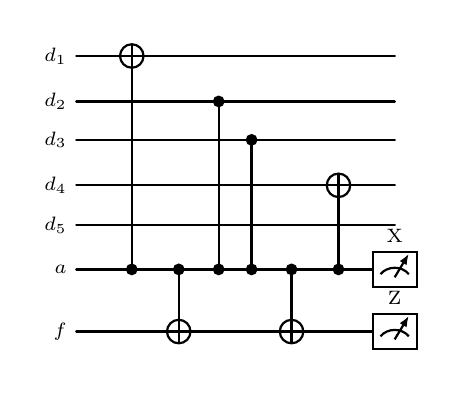
\begin{tikzpicture}[
every node/.style={font=\scriptsize},
outbox/.style={
draw,
rounded corners,
align=left,
inner sep=5pt,
minimum width=6.4cm
}
]

\node (circ) {
  \begin{quantikz}[row sep=0.34cm, column sep=0.27cm, wire types={q,q,q,q,q,q,q}]
    \lstick{$d_1$} & \qw & \targ{}   & \qw        & \qw        & \qw       & \qw       & \qw         & \qw \\
    \lstick{$d_2$} & \qw & \qw       & \qw        & \ctrl{4}   & \qw       & \qw       & \qw         & \qw \\
    \lstick{$d_3$} & \qw & \qw       & \qw        & \qw        & \ctrl{3}  & \qw       & \qw         & \qw \\
    \lstick{$d_4$} & \qw & \qw       & \qw        & \qw        & \qw       & \qw       & \targ{}     & \qw \\
    \lstick{$d_5$} & \qw & \qw       & \qw        & \qw        & \qw       & \qw       & \qw         & \qw \\
    \lstick{$a$}   & \qw & \ctrl{-5} & \ctrl{1}   & \control{} & \control{}& \ctrl{1} & \ctrl{-2}   & \meter{$X$} \\
    \lstick{$f$}   & \qw & \qw       & \targ{}    & \qw        & \qw       & \targ{}   & \qw         & \meter{$Z$}
  \end{quantikz}
};

\end{tikzpicture}
\end{adjustbox}
\caption{A flagged circuit of $XZZXI$.}
\label{fig:flagged-circuit}

\end{wrapfigure}


A basic syndrome extraction circuit alone cannot prevent fault-induced high-weight Pauli error propagation events. The resulting errors may not be reliably characterized from the syndrome alone, which can cause error correction to fail. To address this issue, flagged fault-tolerant error correction augments a basic syndrome extraction circuit with additional ancilla qubits~\cite{CR18a,CR18b}, called \emph{flag qubits}, such as the qubit labeled $f$ in Fig.~\ref{fig:flagged-circuit}, to detect such error propagation events.  The resulting circuit is referred to as a flagged syndrome extraction circuit. 
A flagged syndrome extraction circuit is required to satisfy the validity condition in Def.~\ref{def:syndrome-extraction-valid}. 



 \yfc{Replace this paragraph with one sentence saying that flags detect
fault-induced errors whose minimum weight exceeds the number of faults.
The following definition already gives the precise condition.}
Flag qubits provide additional measurement information that allows the decoder to identify and distinguish high-weight errors induced by a small number of faults. When a given number of faults causes a data error of equal or lesser weight, the error remains correctable as long as the total weight does not exceed the bound t. However, if faults propagate to cause a data error with a weight strictly greater than the number of faults (e.g., a single fault causing a multi-qubit error), it can lead to a logical failure. Therefore, we require the flag measurement to trigger whenever the resulting data error has a weight exceeding the number of faults that occurred in the syndrome extraction circuit.
\begin{definition}[$\cS$-Flag condition] \label{def:flag}
A syndrome extraction circuit satisfies the $\cS$-flag condition if, whenever  an event involving $w \le s$ faults induce a data error $E_{\mathrm{data}}$ such that $\mathrm{wt}_{\min} (E_{\mathrm{data}}) > w$, at least one flag measurement outcome is $1$.
\end{definition}




% Therefore, the flag outcomes are included in the measurement record, and the fault-tolerance of a flagged error correction protocol can be verified using the criterion in Def.~\ref{def:weak-FTEC}.

%\cy{add a flag circuit here; or move Fig 7b here}

A \textit{flagged fault-tolerant error correction protocol} consists of flagged syndrome extraction circuits and syndrome extraction circuits together with an adaptive control flow. 

The control flow is represented by a finite decision tree. It determines which syndrome extraction circuit is executed next based on the syndrome and flag outcomes obtained so far and determines when the protocol terminates.
The decision tree enumerates all possible terminating executions of the protocol

\begin{definition}
\label{def:measurement-record-and-residual-error}
For a given execution path, a \emph{measurement record} $m$ is the bit string consisting of all syndrome and flag outcomes observed along that path.
The corresponding residual error set $\mathcal E_m$ consists of all data Pauli errors consistent with $m$ that can arise from fault events involving at most $t$ faults, prior to decoding.
\end{definition}


Therefore, each execution of the protocol follows a specific control-flow path, executing a sequence of syndrome extraction circuits conditioned on intermediate outcomes. Upon termination, a lookup-table decoder maps the observed measurement record $m$ to a Pauli correction applied to the data qubits.

% \rmark{
% For example, a terminating path may have already accounted for $t$ faults, so that a final full syndrome extraction round can be regarded as fault-free under the assumed fault bound. Alternatively, if $w$ faults have already been accounted for, then observing $t-w+1$ consecutive identical full syndrome outcomes guarantees that the repeated syndrome is reliable~\cite{CB18}. Other adaptive protocols may employ different termination criteria to ensure that sufficient information has been accumulated before applying the recovery operation~\cite{Liou25,TPB23,BSE+23}.
% }

% \rmark{
% In this work, the adaptive control flow of a protocol is assumed to be
% given and correctly specified, meaning that the decision tree enumerates all
% possible terminating executions of the protocol. Specifically, we assume that every terminating path has accumulated sufficient information to perform a reliable error correction that projects the data block back into the code space, possibly leaving only undetected residual data errors.
% }
% \bw{add fault <t?}
In this work, we follow the logic of \cite{CB18} to define the \textit{validity of a control flow.}
\begin{definition}[\textbf{Validity of a control flow}]
\label{def:control-flow-validity}
Consider a control flow of a flagged error correction protocol. We say a control flow is valid if every path of the control flow satisfies one of the following conditions when there are at most $t $ faults :
\begin{enumerate}
   
    \item \textbf{Condition 1:} The measurement  record indicates that $t$ faults have been detected.
    \item \textbf{Condition 2:} A number of faults $w < t$ has been detected, and the protocol subsequently yields an identical full syndrome for $t-w+1$ consecutive extraction rounds without any flag qubit raised.
    \item  \textbf{Condition 3:} For every in put error $E$ with $wt(E) =r$ and  fault event involving $r + w \le t$ faults, the induced data error has a $\mathrm{wt}_{\mathrm{min}}$ at most $w$.
\end{enumerate}
\end{definition}
Condition 3 corresponds to the case where no additional syndrome information is required, since the residual error is already guaranteed to be correctable.

Fig.~\ref{fig:five-qubit-flagged-protocol} illustrates a control flow  of  flagged protocol on the $[[5,1,3]]$ code where $d=3$, $t= \lfloor \frac{3-1}{2 } \rfloor$. 

% For protocols with small code distance, the completeness of such a decision tree can be verified by
% exhaustive enumeration of all possible measurement outcomes and fault
% events.




\begin{figure}[tb]
    \centering

    \begin{adjustbox}{max width=0.8\textwidth,valign=t}
    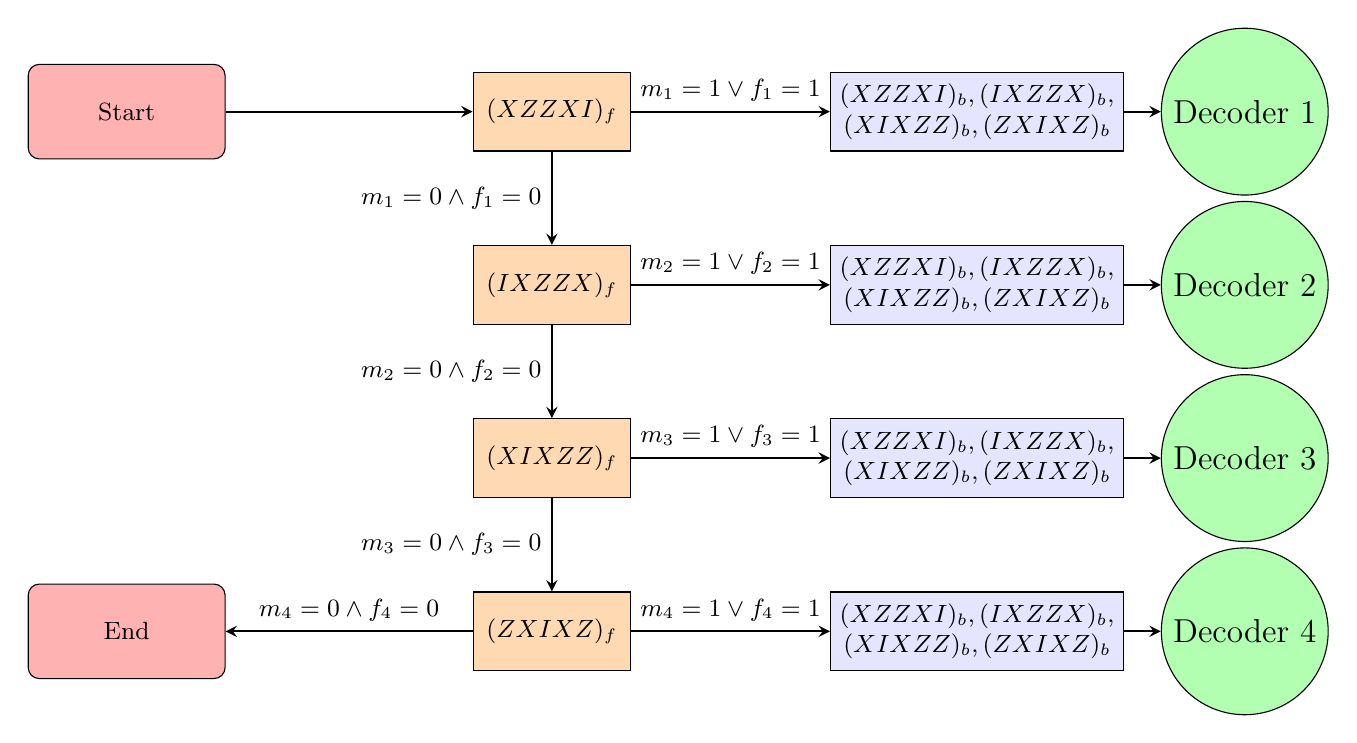
\begin{tikzpicture}[node distance=1.2cm, font=\small] 
        
        % --- 1. Define Styles ---
        \tikzstyle{startstop} = [rectangle, rounded corners, minimum width=2.5cm, minimum height=1.2cm, text centered, draw=black, fill=red!30, font=\small]
        \tikzstyle{raw_syn} = [rectangle, minimum width=2cm, minimum height=1cm, text centered, align=center, draw=black, fill=blue!10, font=\small]
        \tikzstyle{flag_syn} = [rectangle, minimum width=2cm, minimum height=1cm, text centered, align=center, draw=black, fill=orange!30, font=\small]
        \tikzstyle{decode} = [circle, minimum width=2cm, minimum height=1cm, text centered, align=center, draw=black, fill=green!30, font=\large]
        \tikzstyle{arrow} = [thick,->,>=stealth, font=\small]

        % --- 2. Place Nodes ---
        \node (start) [startstop] {Start};
        
        % --- Step 1 ---
        \node (pro1) [flag_syn, right of=start, xshift=4.2cm] {$(XZZXI)_{f}$};
        \node (pro2b) [raw_syn, right of=pro1, xshift=4.2cm] {$(XZZXI)_b, (IXZZX)_b,$\\$(XIXZZ)_b,(ZXIXZ)_b $};
        \node (decode1) [decode, right of=pro2b, xshift=2.2cm] {Decoder 1};
        
        % --- Step 2 ---
        \node (pro2a) [flag_syn, below of=pro1, yshift=-1cm] {$(IXZZX)_{f}$};
        \node (pro3b) [raw_syn, right of=pro2a, xshift=4.2cm] {$(XZZXI)_b, (IXZZX)_b,$\\$(XIXZZ)_b,(ZXIXZ)_b $};
        \node (decode2) [decode, right of=pro3b, xshift=2.2cm] {Decoder 2};

        % --- Step 3 ---
        \node (pro3a) [flag_syn, below of=pro2a, yshift=-1cm] {$(XIXZZ)_{f}$};
        \node (pro4b) [raw_syn, right of=pro3a, xshift=4.2cm] {$(XZZXI)_b, (IXZZX)_b,$\\$(XIXZZ)_b,(ZXIXZ)_b $};
        \node (decode3) [decode, right of=pro4b, xshift=2.2cm] {Decoder 3};

        % --- Step 4 ---
        \node (pro4a) [flag_syn, below of=pro3a, yshift=-1cm] {$(ZXIXZ)_{f}$};
        \node (pro5b) [raw_syn, right of=pro4a, xshift=4.2cm] {$(XZZXI)_b, (IXZZX)_b,$\\$(XIXZZ)_b,(ZXIXZ)_b $};
        \node (decode4) [decode, right of=pro5b, xshift=2.2cm] {Decoder 4};

        % End
        \node (stop) [startstop, left of=pro4a, xshift=-4.2cm] {End};

        % --- 3. Draw Arrows ---
        \draw [arrow] (start) -- (pro1);
        
        \draw [arrow] (pro1) -- node[left] {$m_1=0 \wedge f_1=0$} (pro2a);
        \draw [arrow] (pro1) -- node[above,xshift= 0cm, yshift = 0cm] {$m_1=1 \vee f_1=1$} (pro2b);
        \draw [arrow] (pro2b) -- (decode1);

        % From Step 2
        \draw [arrow] (pro2a) -- node[left] {$m_2=0 \wedge f_2=0$} (pro3a);
        \draw [arrow] (pro2a) -- node[above,xshift= 0cm, yshift = 0cm] {$m_2=1 \vee f_2=1$} (pro3b);
        \draw [arrow] (pro3b) -- (decode2);

        % From Step 3
        \draw [arrow] (pro3a) -- node[left] {$m_3=0 \wedge f_3=0$} (pro4a);
        \draw [arrow] (pro3a) -- node[above,xshift= 0cm, yshift = 0cm] {$m_3=1 \vee f_3 =1$} (pro4b);
        \draw [arrow] (pro4b) -- (decode3);
        
        % From Step 4
        \draw [arrow] (pro4a) -- node[above ,xshift= 0cm, yshift = 0cm] {$m_4=1 \vee f_4=1$} (pro5b);
        \draw [arrow] (pro4a) -- node[above, yshift = 0cm] {$m_4=0 \wedge f_4=0$} (stop);
        \draw [arrow] (pro5b) -- (decode4);

    \end{tikzpicture}
    \end{adjustbox}

    \caption{A flagged error correction protocol for the $[[5,1,3]]$ code where $t = 1$, adapted from~\cite{Chao18}. A label $(P)_f$ denotes the flagged syndrome extraction circuit for stabilizer $P$, while $(P)_b$ denotes the corresponding basic syndrome extraction circuit. Each path from the $\mathrm{Start}$ to the $\mathrm{Decoder}$ satisfies Condition (1) in Def~\ref{def:control-flow-validity}. This is because, along each such path, at least one of the outcomes ($m_i$ or $f_i$) is $1$, indicating the presence of at least one fault or input error, and the four syndrome extractions are sufficient to ensure all resulting errors are syndrome-consistent. The path from $\mathrm{Start}$ to $\mathrm{End }$ will satisfies  Condition (3) in Def~\ref{def:control-flow-validity}   since non of the flag raised.}
\bw{changed condition(1) to condition (3)}
\yfc{Please check whether the absence of flags is sufficient to establish
Condition (3) on this path, including the case $r=1,s=0$.}
\bw{yes when r =1 it will never come to this path at least one syndrome will be 1 }
    \label{fig:five-qubit-flagged-protocol}
\end{figure}

Since the purpose of flag qubits is to signal high-weight error propagation events, we introduce the flag condition in the following.



% We emphasize that a flagged error correction protocol for a distance $d$ QECC does not strictly require its circuits to satisfy the full $t$-flag condition where $t = \lfloor \frac{d-1}{2} \rfloor$. Depending on the design of the control flow, a weaker condition may suffice. Specifically, paths terminating via Condition 2 of Definition~\ref{def:control-flow-validity} only need to satisfy a reduced $(t-w)$-flag condition (Definition~\ref{def:flag}). For example, in the $[[19,1,5]]$ protocol presented in~\cite{Liou25}, the control flow guarantees that any path satisfying Condition 2 will have already detected at least one fault ($w \geq 1$). Consequently, for $t=2$, the constituent circuits only need to satisfy a $1$-flag condition.



% \rmark{
% We emphasize that satisfying Def.~\ref{def:flag} is not a necessary condition for a flagged fault-tolerant error correction protocol. In some cases, the measurement record may contain sufficient information to distinguish and correct the resulting errors even when the flag condition is violated~\cite{Liou25}. An example is the $[[19,1,5]]$ protocol presented in Section~4, which is fault-tolerant but does not satisfy the flag condition.
% }


% Therefore, in this subsection, we verify that a flagged error correction protocol satisfies FTEC using a two-step approach. First, we define the validity of a protocol. Second, we determine if there is any possibility of a logical error occurring under this protocol. If both conditions are satisfied, we can formally guarantee via a theorem that the flagged error correction protocol satisfies Def~\ref{def:weak-FTEC}.
% To evaluate the validity of the control flow, we first define an error set associated with a given measurement record:
% \begin{definition} \bw{Dont need defintion env}
%     For each path and every measurement record $m$ from a fault event with at most $t$ faults, we define $\mathcal{E}_m$ as the error set containing all possible remaining data errors. 
% \end{definition}

% To establish that a path of the control flow satisfies Condition (1) of Def~\ref{def:control-flow-validity}, we must verify that for every measurement record $m$ along that path, the error set $\mathcal{E}_m$ is syndrome-consistent—meaning that all errors within the set share the same ideal syndrome.

% To establish that a path satisfies Condition (2), we only need to verify that at least $w$ faults have occurred , followed by $t-w+1$ consecutive full syndrome extraction rounds yielding identical results without any flag raised. %In this scenario, we do not rely on the error set $\mathcal{E}_m$.


% The preceding discussion distinguishes the information used for recovery in the
% different termination cases. We now define the class of decoders that act
% according to these cases.


% \begin{definition}
%     For a flagged error correction protocol, a \textit{suitable decoder} is one that, for each path satisfying Condition (1) or (2) in Def~\ref{def:control-flow-validity} with measurement record $m$, outputs a correction $C \in \mathcal{E}_m$. For any path satisfying Condition (3) in Def~\ref{def:control-flow-validity}, the decoder outputs a trivial correction (i.e., applying the identity operator to all data qubits).
% \end{definition}\label{def:decoder}

% The definition only specifies the required behavior of the decoder in each
% termination case. The next lemma shows that, if the control flow is valid 
% (Def.~\ref{def:control-flow-validity}), such a decoder is well defined.



% \begin{lemma}
%     For any flagged error correction protocol whose control flow satisfies Definition~\ref{def:control-flow-validity}, a suitable decoder always exists.
% \end{lemma}

% \begin{proof}
%     For any fault event of weight $\leq t$, consider any path in the control flow that satisfies either Condition (1) or (2) of Definition~\ref{def:control-flow-validity}. Because these conditions are met, the corresponding error set $\mathcal{E}_m$ associated with the measurement record $m$ is guaranteed to be non-empty. Consequently, there always exists at least one valid correction operator $C \in \mathcal{E}_m$. For any path satisfying Condition (3), we can unconditionally assign a trivial correction (the identity operator). Thus, a suitable decoder can always be constructed for the protocol. 
% \end{proof}

The preceding definitions specify when a flagged error correction protocol is
well formed for the purpose of fault-tolerant recovery: the extraction circuits must provide valid measurement records, the control flow must terminate in one of the intended cases, and the flag condition must hold whenever the argument relies on unflagged full syndrome extraction rounds (Condition 2). We collect these requirements into a single protocol-level validity condition.

\begin{definition}
\label{def:protocol-validity}
A flagged error correction protocol is valid if all the following condition satisfies:
\begin{enumerate}
    \item All syndrome extraction circuits used in this protocol are valid (Def \ref{def:syndrome-extraction-valid}).
    \item The control flow of the protocol is valid (Def \ref{def:control-flow-validity}).
    \item For each path of the control flow satisfying the Condition (2) of Def~\ref{def:control-flow-validity} and has detected $w$ faults, the full syndrome extraction circuit needs to satisfies $(t-w)$-flag condition (Def.~\ref{def:flag}). 
\end{enumerate}
\end{definition}



% Each internal node represents a syndrome extraction circuit, and each outgoing edge is labeled by a branch condition on the syndrome and flag outcomes. A terminating path determines the corresponding measurement record. In this example,
% The paths ending at Decoder 1--4 satisfy termination condition (2). The branch condition $m_i=1 \vee f_i=1$ indicates that at least one fault has been detected, so $w=1$. Since $t-w+1=1$, condition (2) requires only one full syndrome extraction circuit in the terminating suffix; this is the blue node immediately before the decoder. The path ending at the End node satisfies
% termination condition (3).
For a valid flagged error correction protocol, a critical question remains: even if the measurement record provides sufficient information for a lookup-table decoder, are there cases where applying the chosen correction still violates FTEC (Definition~\ref{def:weak-FTEC}). The following theorem provides the core characterization of this property: a valid flagged error correction protocol achieves FTEC if and only if, for any given measurement record $m$, no two possible residual errors associated with $m$ multiply to form a non-trivial logical operator. This precise characterization serves as the foundation for our verification algorithm presented in Section~\ref{sec:FTEC-verification}.

% \begin{theorem}
% \label{thm:mains}
%  Consider a flagged error correction protocol $\Pi$ for a stabilizer code
% with stabilizer group $\cS$, distance $d$, and
% $t=\lfloor (d-1)/2 \rfloor$. Assume that $\Pi$ is valid in the sense of Def.~\ref{def:protocol-validity} and the path satisfies condition (1)  Def \ref{def:control-flow-validity} has all residual error  with same ideal syndrome while the measurement record are the same.
% Then there exists a suitable lookup-table decoder $D$ such that $(\Pi,D)$ satisfies
% FTEC if and only if, for all measurement record $m$,
% $\forall E_1,E_2\in \mathcal{E}_{m},
%     E_1E_2 \notin N(\cS)\setminus S$.  
% \end{theorem}

\begin{theorem}
\label{thm:mains}
\yfc{Please check the consistency of the assumptions in this theorem,
the appendix theorem, and Algorithm~\ref{alg:ftec-verification}, especially
the role of Condition (1).}
Consider a flagged error-correction protocol $\Pi$ for a stabilizer
code with stabilizer group $\cS$, distance $d$, and
$t=\lfloor (d-1)/2 \rfloor$. Assume that $\Pi$ is valid in the sense of
Def.~\ref{def:protocol-validity}, and that Condition~(1) of
Def.~\ref{def:control-flow-validity} holds, so that all residual
errors corresponding to the same measurement record have the same
ideal syndrome. For each measurement record $m$, let
$\mathcal{E}_m$ denote the set of residual errors consistent with $m$.
Then there exists a lookup-table decoder $D$ such that $(\Pi,D)$
satisfies FTEC if and only if, for every measurement record $m$,
\begin{align}
    \forall E_1,E_2\in\mathcal{E}_m,\qquad
    E_1\cdot  E_2\notin N(\cS)\setminus \cS.
\end{align}
\end{theorem}




\begin{proof}[Proof sketch]
\yfc{After resolving the correctness comments, shorten the forward direction
to the single inequality d>2t and its contradiction. Keep one sentence
per termination condition in the reverse direction, including the actual
residual-weight bound; leave the detailed derivations in the appendix.}
The full proof of this theorem is in Appendix~\ref{app:proof} of the supplementary material. \\


\textbf{($\Rightarrow$)}
Suppose, by contradiction, that there exist two residual errors
$E_1,E_2\in\mathcal{E}_m$ such that
$E_1\cdot E_2$ is a non-trivial logical operator, i.e.,
$E_1\cdot E_2\in N(\cS)\setminus \cS$.
If the decoder applies a correction $C$, then the product of the
two corrected errors is $(E_1\cdot C)\cdot (E_2\cdot C)=E_1\cdot E_2.$
Since $E_1\cdot E_2$ is a non-trivial logical operator,
$\mathrm{wt}_{\min}(E_1\cdot E_2)\ge d>2t. $
On the other hand, if both corrected errors satisfied the FTEC
weight requirement, then
$\mathrm{wt}_{\min}(E_1\cdot C)\le t$ and $ \mathrm{wt}_{\min}(E_2\cdot C)\le t,$
which would imply
$\mathrm{wt}_{\min}(E_1\cdot E_2) =\mathrm{wt}_{\min}\bigl((E_1\cdot C)\cdot (E_2\cdot C)\bigr)
\le \mathrm{wt}_{\min}(E_1\cdot C)
+\mathrm{wt}_{\min}(E_2\cdot C)
\le 2t,$
a contradiction. Therefore, at least one of the two corrected errors
violates the FTEC weight requirement, and the protocol cannot achieve
FTEC.



\textbf{($\Leftarrow$)} Assuming $\forall E_1, E_2 \in \mathcal{E}_m, E_1 \cdot E_2 \notin N(\cS) \setminus \cS$, we show the protocol satisfies FTEC across the three termination conditions of a valid protocol (Def.~\ref{def:protocol-validity}):
\begin{itemize}
    \item \textbf{Condition (1):} All residual errors in $\mathcal{E}_m$ share the same ideal  syndrome, so for any decoder choice $C \in \mathcal{E}_m$, $E \cdot C$ commutes with the stabilizers. By our assumption, $E \cdot C \in S$, meaning the logical state is preserved.
    \item \textbf{Condition (2):} The protocol terminates after $t-w+1$ repeated full-syndrome rounds without flags. With at most $t-w$ faults remaining, at least one round $R$ must be fault-free. The data error $E^-$ before $R$ produces the syndrome precisely and will belong to the equivalence class represented by the decoder choice $C$. The final error is $C \cdot E^- \cdot E_{\mathrm{suf}} \sim E_{\mathrm{suf}}$. Because no flags were raised and at most $s-w$ faults occurred after $R$, the  $\mathrm{wt}_{\mathrm{min}}$ of final error is bounded by $  s \le t$, satisfying FTEC.
    \item \textbf{Condition (3):} If the protocol stops, the resulting error $E \in \mathcal{E}_m$ naturally satisfies $\mathrm{wt}_{min}(E) \le t$. An ideal decoder will successfully recover the state since the total error weight remains within the code's correctable limit, satisfying FTEC.
    \yfc{Old version: Condition (3) is not a maximum-round stopping rule.
    Use the residual-weight bound $s$ (circuit faults), not $t$, for $r+s\le t$.}
\end{itemize}

\end{proof}






% \subsection{Verification of flagged fault-tolerant error correction protocols}
% \label{subsec:verification}
% In this subsection, we discuss the verification of a flagged fault-tolerant error correction protocol.

% A flagged fault-tolerant error correction protocol is an adaptive
% procedure whose execution is determined by a decision tree. Each internal
% node of the tree specifies a syndrome extraction circuit, and each outgoing
% edge is conditioned on the measurement outcomes obtained from that circuit.
% A terminating path therefore represents one possible execution of the
% protocol and determines a measurement record available to the decoder.


% % \rmark{
% % In this work, the adaptive control flow of a protocol is assumed to be
% % given and correctly specified, meaning that the decision tree enumerates all
% % possible terminating executions of the protocol. Specifically, we assume that every terminating path has accumulated sufficient information to perform a reliable error correction that projects the data block back into the code space, possibly leaving only undetected residual data errors.
% % }

% % \rmark{
% % For example, a terminating path may have already accounted for $t$ faults, so that a final full syndrome extraction round can be regarded as fault-free under the assumed fault bound. Alternatively, if $w$ faults have already been accounted for, then observing $t-w+1$ consecutive identical full syndrome outcomes guarantees that the repeated syndrome is reliable~\cite{CB18}. Other adaptive protocols may employ different termination criteria to ensure that sufficient information has been accumulated before applying the recovery operation~\cite{Liou25,TPB23}.
% % }

% % For protocols with small code distance, the completeness of such a decision tree can be verified by
% % exhaustive enumeration of all possible measurement outcomes and fault
% % events.



% Under the equivalent fault model in Proposition~\ref{prop:simplified_noise},
% the fault-tolerant conditions can be stated as follows.

% \begin{definition} \label{def:FTEC_simplified}
% Let $\mathcal{Q}$ be an $[[n,k,d]]$ stabilizer code with
% $t=\lfloor (d-1)/2\rfloor$.
% An error correction protocol is \emph{fault-tolerant up to $t$ faults}
% if the following conditions are satisfied.

% \begin{enumerate}
% \item (correction)
% For every fault event involving at most $t$ faults, the residual data
% error after applying the correction determined by the measurement record
% is correctable by an ideal decoder.

% \item (fault containment)
% For every fault event involving $s\le t$ faults, the residual data error
% $E_{\mathrm{res}}$ after applying the correction determined by the
% measurement record satisfies
% \[
% \mathrm{wt}(E_{\mathrm{res}})\le s .
% \]
% \end{enumerate}
% \end{definition}


% The goal of verification is not to verify a preassigned decoder. Instead,
% we verify whether the measurement records generated by the protocol admit a
% lookup-table decoder satisfying the fault-tolerance conditions in~Def.~\ref{def:FTEC_simplified}. Therefore, the decoder correction associated with each measurement record is not assumed
% in advance but is determined by the distinguishability of possible fault
% events.


% \subsubsection{Verification of the correction condition}

% An execution of an error correction protocol is simulated as follows.
% Consider an execution with a set of circuit faults $F$, which induce a
% Pauli error $E$ on the data qubits. The execution produces a measurement
% record $m(F)$. The decoder $\cD$ observes only this measurement record and
% assigns a Pauli correction
% \[
% C=\cD(m(F))
% \]
% to the data block. The residual error after correction is therefore
% $CE$. Let
% \[
% z=\mathrm{syn}(CE)
% \]
% denote the ideal syndrome of the residual error as defined in
% (\ref{eq:syndrome}).

% We have the following operational proposition for condition (1)  of Def.~\ref{def:FTEC_simplified}.
% \begin{proposition} \label{prop:correction}
% A flagged error correction protocol with fault bound $t$ satisfies
% condition (1) of Def.~\ref{def:FTEC_simplified} if and only if,
% for any two executions involving no more than $t$ faults, whenever their
% measurement records are identical, their residual errors satisfy the
% quantum error correction condition. 
% \end{proposition}



% \begin{proof}
% (Sufficient)
% Consider two executions with at most $t$ faults. Let their induced data
% errors, measurement records, corrections, residual errors, and ideal
% syndromes be denoted by
% \[
% (E_1,m_1,C_1,C_1E_1,z_1)
% \quad
% \mbox{ and }\quad
% (E_2,m_2,C_2,C_2E_2,z_2),
% \]
% respectively, where $C_i=\cD(m_i).$



% If $m_1\neq m_2$, the two executions are distinguishable by the decoder,
% and therefore they can be assigned different corrections.

% Consider the case $m_1=m_2$. Since the decoder observes the same
% measurement record, we have
% \[
% C_1=C_2.
% \]
% The residual errors $C_1E_1$ and $C_2E_2$ are simultaneously correctable
% by an ideal decoder if and only if
% \begin{align}
% (C_1E_1)^\dagger(C_2E_2)
% \notin N(\mathcal S)\setminus\mathcal S,
% \label{eq:CE_QEC}
% \end{align}
% up to global phases, according to the quantum error correction
% condition~in Eq.~(\ref{eq:QECC_condition}).

% If $z_1\neq z_2$, then $(C_1E_1)^\dagger(C_2E_2)\notin N(\mathcal S)$,
% which satisfies Eq.~(\ref{eq:CE_QEC}). Hence, the two residual errors are
% distinguishable by an ideal decoder.

% If $z_1=z_2$, the two residual errors have the same syndrome. In this
% case, Eq.~(\ref{eq:CE_QEC}) is satisfied only when $
% (C_1E_1)^\dagger(C_2E_2)\in\mathcal S.
% $  Since $C_1=C_2$, this condition reduces to
% $
% E_1^\dagger E_2\in\mathcal S,
% $ 
% up to global phases.

% Therefore, for every pair of executions with the same measurement
% record and the same ideal syndrome, their residual errors must differ
% only by stabilizers. Under this condition, all possible residual errors
% associated with a measurement record are correctable by the decoder,
% which proves condition (1)  of Def.~\ref{def:FTEC_simplified}.


% (Necessary)
% Suppose there exist two executions with the same measurement record
% $m_1=m_2=m$ such that $
% E_1^\dagger E_2\in N(\mathcal S)\setminus\mathcal S .
% $
% Since the decoder observes the same measurement record, it applies the
% same correction operator $C=\mathcal D(m)$ to both executions.
% However, the resulting residual errors differ by $(CE_1)^\dagger(CE_2)=E_1^\dagger E_2$,
% which is a nontrivial logical operator. Therefore, these two residual
% errors cannot be simultaneously corrected by an ideal decoder, violating
% condition (1) of Def.~\ref{def:FTEC_simplified}.


% \end{proof}

% \textbf{Remark}. In practice, the above condition can be verified pairwise.
% Consider two executions with residual errors $R_1$ and $R_2$. If their measurement records are different, they are assigned different corrections and therefore require no further comparison.

% Suppose the two executions have the same measurement record.
% If their ideal syndromes are different, then $R_1$ and $R_2$ are already
% distinguishable by an ideal decoder. Only the case in which both the measurement records and the ideal
% syndromes coincide requires verification.
% In this case, 
% \[
% (C_1E_1)^\dagger(C_2E_2)
% =
% E_1^\dagger E_2,
% \]
% because $C_1=C_2$.
% Hence, it suffices to verify that
% \[
% E_1^\dagger E_2\in\mathcal S,
% \]
% up to global phases.

% Equivalently, when two executions have the same measurement record, their
% ideal syndromes must be distinguishable unless their residual errors are
% equivalent up to stabilizers.



% \subsubsection{Verification of the fault containment condition}

% \bmark{The second requirement ensures that fault propagation during syndrome extraction leaves only a bounded residual data error after correction.}

% \bmark{By Proposition~\ref{prop:simplified_noise}, it is sufficient to consider Pauli faults inserted at two-qubit gate locations. Each such fault is represented by one of the 15 non-identity two-qubit Pauli operators, such a $IX$, $XY$, or $ZZ$, inserted after the ideal gate. We refer to each such elementary two-qubit Pauli errors a \emph{fault component}. Since syndrome extraction circuits consist of Clifford operations, each fault component can be propagated independently through the circuit. We call a fault component \emph{undetected} on a path if an execution with only this fault component produces an all-zero measurement record.}


% An undetected fault component cannot be identified from the measurement
% record and therefore cannot be specifically removed by the recovery
% operation. 

% On the other hand, a fault event on a path of $N$ locations can be represented by a $2N$ binary vector
% $(P_{1x}, P_{1z},\dots, P_{Nx}, P_{Nz})$ as in Eq.~(\ref{eq:binary}).
% A fault component corresponding to an elementary basis vector in the binary representation 
% is called a fault basis vector, such as $XI$, $IX$, $ZI$, $IZ$ at a location on the path.
% A fault basis vector has with measurement record zero is called an undetected basis. 

% \rmark{
% In this work, the adaptive control flow of a protocol is assumed to be
% given and correctly specified, meaning that the decision tree enumerates all
% possible terminating executions of the protocol. Specifically, we assume that every terminating path has accumulated sufficient information to perform a reliable error correction that projects the data block back into the code space, possibly leaving only undetected residual data errors due to undetected basis vectors.
% Equivalently, we assume that a fault vector consisting of solely detectable fault basis vectors 
% will leave a residue error with ideal syndrome zero after correction based on its measurement record.
% }

% \begin{definition} \label{def:legitimate}
% A control flow is called \emph{syndrome-complete} if, for every terminating path,
% the recovery operation maps any fault event involving at most $t$ faults
% and consisting solely of detectable fault basis vectors to a residual error
% with zero ideal syndrome.
% \end{definition}
% The syndrome-complete property does not require the residual error to be
% trivial or logically correct; it only requires that all detectable fault
% contributions are removed at the syndrome level.

% Consequently, undetected fault components are the only possible source
% of residual errors after the terminating error correction procedure.




% \begin{proposition} \label{prop:containment}
% Consider a flagged error correction protocol with fault bound $t$ and a syndrome-complete control flow.
% Then condition
% (2) of Def.~\ref{def:FTEC_simplified} is satisfied if and only if every
% undetected fault component on every terminating path induces at most one
% residual data error.
% \end{proposition}



% \begin{proof}
% % We first show that only undetected fault basis elements need to be
% % considered. Let a fault event be decomposed into fault basis elements.
% % Suppose a combination of detectable fault basis elements produces an
% % all-zero measurement record. This execution has the same measurement record
% % as the fault-free execution. Therefore, by condition (1), the residual error
% % of this execution and the identity residual error from the fault-free
% % execution must satisfy the quantum error correction condition. Hence, the
% % residual error induced by this combination must be a stabilizer (up to
% % global phases) and does not contribute to a nontrivial residual data error.

% Only undetected fault components need to be considered for
% the fault containment condition. If each undetected fault component
% induces at most one residual data error, then an event containing $\cS$ faults
% can induce at most $\cS$ residual errors, and hence
% $
% \mathrm{wt}(E_{\mathrm{res}})\le s.
% $

% Conversely, suppose condition (2) holds. Consider an execution containing a
% single undetected fault component. Since this corresponds to $s=1$
% fault, condition (2) requires that the resulting residual error satisfies
% $
% \mathrm{wt}(E_{\mathrm{res}})\le 1 .
% $
% Therefore, every undetected fault component induces at most one residual
% data error.


% \end{proof}


% \begin{proposition}
%     For a control flow if each path satisfies:
%     \begin{itemize}
%         \item Ter1:Distinguible : For any two fault events that has at most t faults, if they have the same measurement record then the residual error should have same ideal syndrome.
%         \itemTer2: There are at most $w$ fault in the path and $w < t $ and there  are $t-w+1$ consecutive identical full syndrome with no flag raised.
        
%     \end{itemize}
%     then the protocol is syndrome complete.
    
% \end{proposition}

% \begin{proof}
%     \begin{itemize}
%         \item Ter1 : If a path is distinguishable $\Rightarrow$ For any tow fault event consist of fault basis have same measurement record the nthe residual errr have same ideal syndrome $\Rightarrow $  For any tow fault event consist of detectable fault basis have same measurement record the the residual errr have same ideal syndrome $\Rightarrow$  For any tow fault event consist of detectable fault basis have same measurement record there exist a correction $C$ that have the same ideal syndrome with the two resisidual errors $\Rightarrow $  For any tow fault event consist of detectable fault basis have same measurement record after the corection $C$ the residual error will have zero ideal syndrome 
%         \item Ter2: Claim : For all  fault event satisfies the path condition and  consist of detectable fault basis there is a recovery operation such that the residual errro aafter correction has ideal syndrome all zero.
%         Let $f$ be a fault  event  that satisfies the path condition and is consist of a set of detectable fault basis $\{v_{det}\}$, that is $f = \sum_{v_j \in \{v_{det}\}}  v_j$
%         If every basis in $\{v_{det} \}$ happens before the $t-w+1$ full snydroem extraction circuit then the $t-w+1 $ consectutive syndorme  is fault free so the consecutive will equal the ideal syndrome of the error entering the consecutive syndrome extraction circuit.
%         If there are  basis in $\{v_{det} \}$ that happens in the consecutive synforme extraction, and one of the flagged raised $\rightarrow \leftarrow $
%         If there are  basis in $\{v_{det} \}$ that happens in the consecutive synforme extraction, no of the flagged raised  but the $t-w+1 $consecutive syndroem are different $\rightarrow \leftarrow $

%         If there are  basis in $\{v_{det} \}$ that happens in the consecutive syndorme extraction, none of the flagged raised $\rightarrow \leftarrow $, and the consecutive syndrome are 
        
        
%     \end{itemize}
% \end{proof}















\clearpage




\section{FTEC Verification Algorithm}
\label{sec:FTEC-verification}

\begin{wrapfigure}[14]{r}{0.45\textwidth}
\vspace{-1.2em}
\centering
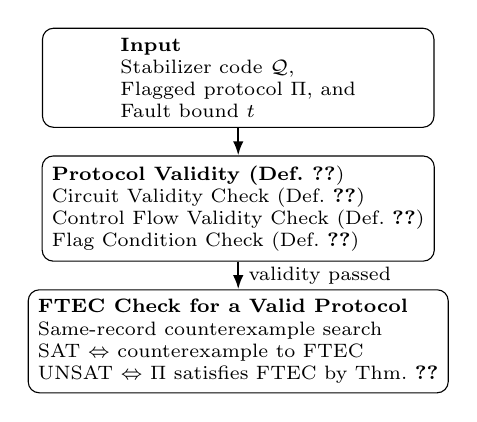
\begin{tikzpicture}[
  node distance=0.35cm,
  every node/.style={font=\scriptsize},
  box/.style={
    draw,
    rounded corners,
    align=left,
    inner sep=3.5pt,
    minimum width=0.41\textwidth
  },
  arrow/.style={
    -{Latex[length=1.8mm]},
    thick
  }
]

\node[box] (input) {
\textbf{Input}\\
Stabilizer code $\mathcal{Q}$, \\
Flagged protocol $\Pi$, and\\
Fault bound $t$
};

\node[box, below=of input] (circuit) {
\textbf{Protocol Validity (Def.~\ref{def:protocol-validity}})\\
Circuit Validity Check (Def.~\ref{def:syndrome-extraction-valid})\\
Control Flow Validity Check (Def.~\ref{def:control-flow-validity})\\
Flag Condition Check (Def.~\ref{def:flag})
};

\node[box, below=of circuit] (protocol) {
\textbf{FTEC Check for a Valid Protocol}\\
Same-record counterexample search\\
SAT $\Leftrightarrow$ counterexample to FTEC\\
UNSAT $\Leftrightarrow$ $\Pi$ satisfies FTEC by Thm.~\ref{thm:mains}
};

\draw[arrow] (input) -- (circuit);
\draw[arrow] (circuit) -- node[right] {validity passed} (protocol);

\end{tikzpicture}
\caption{SAT-based verification pipeline.}
\label{fig:verification-pipeline}
\vspace{-1.0em}
\end{wrapfigure}

This section presents the verification algorithm for checking whether a flagged error correction protocol $\Pi$ satisfies FTEC. The algorithm is based on Thm.~\ref{thm:mains}. It first checks that $\Pi$ is a valid protocol in the sense of Def.~\ref{def:protocol-validity}. It then checks the condition in Thm.~\ref{thm:mains}: no two executions within the fault
bound may produce the same measurement record while leaving residual data errors whose relative error is a nontrivial logical operator.


We organize the presentation by the analysis method used by the verifier. We first present the SAT-based checks, including the SAT formula for the FTEC condition in Thm.~\ref{thm:mains}, circuit correctness check, flag condition, and the control flow validity conditions that are reduced to SAT queries. We then describe the remaining validity checks: circuit determinism is checked by stabilizer simulation, and Condition (2) of Def.~\ref{def:control-flow-validity} is checked by direct inspection of terminating paths. The overall algorithm first establishes protocol validity and then applies the FTEC check.

% \clearpage
% We organize the presentation by the analysis method used by the verifier.
% We first present the SAT-based checks, including the circuit-correctness check (Def \ref{def:syndrome-extraction-correct}), the control-flow validity (Def \ref{def:control-flow-validity}) checks for Conditions~(1) and~(3), the required flag condition (Def \ref{def:flag}) checks, and the final FTEC counterexample search. We then describe
% the remaining validity checks: circuit determinism is checked by stabilizer-tableau simulation, and Condition~(2) of Def.~\ref{def:control-flow-validity} is checked by direct inspection of
% terminating paths.
% \cy{these two pargraphs look the same}

\subsection{SAT-Based Checks}
\label{subsec:sat-based-checks}


\bw{maybe for Fault we include the idle fault at the begin. which can also represent the input error on data qubit}
We first define the symbolic objects used by the SAT-based checks.
The verifier analyzes each terminating path of the protocol separately.
Let $\pi$ be a terminating path, and let $\mathcal{L}_\pi$ denote the set of
fault locations along $\pi$.A \emph{fault assignment} is defined as a tuple $\mathcal{F} = (\mathcal{F}_{\text{in}}, \mathcal{F}_{\text{circ}})$, where $\mathcal{F}_{\text{in}}$ denotes the input data error and $\mathcal{F}_{\text{circ}}$ assigns a Pauli fault to each location in $\mathcal{L}_\pi$.

For a fault location $\ell\in\mathcal{L}_\pi$ acting on qubits $q_1$ and
$q_2$, the Pauli fault is represented by Boolean variables
$x_{\ell,q_1},z_{\ell,q_1},x_{\ell,q_2},z_{\ell,q_2}\in\{0,1\}$,
where the pair $(x_{\ell,q},z_{\ell,q})$ specifies the Pauli component on
qubit $q$. We introduce an activity variable
$a_\ell\in\{0,1\}$ to indicate whether the fault at $\ell$ is nontrivial:
\begin{equation}
a_\ell
\leftrightarrow
x_{\ell,q_1}\vee z_{\ell,q_1}\vee
x_{\ell,q_2}\vee z_{\ell,q_2}.
\end{equation}
Thus, $a_\ell=1$ exactly when the fault assigned to $\ell$ is not the
identity. The fault weight of $\mathcal{F}$ is then
\[
\mathrm{wt}(\mathcal{F})
=
\sum_{\ell\in\mathcal{L}_\pi} a_\ell.
\]
Constraints such as $\mathrm{wt}(\mathcal{F})\le t$ and
$\mathrm{wt}(\mathcal{F})=w$ are encoded using standard cardinality
constraints~\cite{sinz2005towards}.

Given a fault assignment $\mathcal{F}$, the verifier symbolically propagates
the corresponding Pauli faults through the protocol along the terminating path
$\pi$. This propagation determines three objects:
\[
\Phi_\pi(\mathcal{F}),\qquad
E_\pi(\mathcal{F}),\qquad
m_\pi(\mathcal{F}).
\]
Here, $\Phi_\pi(\mathcal{F})$ is the path condition specifying that the
syndrome and flag outcomes produced under $\mathcal{F}$ cause the protocol to
follow the terminating path $\pi$; $E_\pi(\mathcal{F})$ is the residual Pauli
error on the data block at the end of $\pi$; and
$m_\pi(\mathcal{F})$ is the measurement record consisting of the syndrome and
flag outcomes available to the decoder.

The symbolic propagation is performed at the level of individual qubits.
For each qubit $q$, the verifier maintains a symbolic Pauli label
\[
Q_q(\mathcal{F})
=
\bigl(
Q_{q,x}(\mathcal{F}),
Q_{q,z}(\mathcal{F})
\bigr),
\]
where $Q_{q,x}(\mathcal{F})$ and $Q_{q,z}(\mathcal{F})$ are Boolean formulas
over the fault variables and represent the symbolic $X$- and $Z$-components
of the Pauli error on $q$. The gate-by-gate update rules for these symbolic
labels are given in Figure~\ref{fig:two-qubit-pauli-rules}.

At the end of the terminating path $\pi$, restricting these symbolic labels to
the data qubits $d_1,\ldots,d_n$ gives the residual data error
\[
E_\pi(\mathcal{F})
=
\bigl(
Q_{d_1,x}(\mathcal{F}),Q_{d_1,z}(\mathcal{F}),
\ldots,
Q_{d_n,x}(\mathcal{F}),Q_{d_n,z}(\mathcal{F})
\bigr).
\]
The same symbolic propagation determines the syndrome and flag outcomes and
hence the measurement record $m_\pi(\mathcal{F})$ and the path condition
$\Phi_\pi(\mathcal{F})$. Thus, for a fixed terminating path, a fault
assignment is mapped to the symbolic quantities used throughout the SAT
formulation:
\[
\mathcal{F}
\quad\longmapsto\quad
\bigl(
\Phi_\pi(\mathcal{F}),
E_\pi(\mathcal{F}),
m_\pi(\mathcal{F})
\bigr).
\]

This notation makes the dependence of the symbolic quantities on the Boolean
fault variables explicit; it therefore differs slightly from the notation
used in Figure~\ref{fig:syndrome extraction-circuits-2}.

% We first define the symbolic objects used by the SAT-based checks. The verifier
% analyzes each terminating path of the protocol separately. Let $\pi$ be a
% terminating path, and let $\mathcal L_\pi$ be the set of fault locations along
% $\pi$. A fault assignment $\mathcal{F}$ assigns a Pauli fault to each location in
% $\mathcal L_\pi$.
% For each fault location $\ell\in\mathcal L_\pi$ acting on qubits $q_1$ and
% $q_2$, the fault at $\ell$ is represented by Boolean variables $x_{\ell,q_1},z_{\ell,q_1},x_{\ell,q_2},z_{\ell,q_2}$.
% The activity variable of $\ell$ is a Boolean variable
% $a_\ell\in\{0,1\}$ defined by
% \[
% a_\ell\leftrightarrow
% x_{\ell,q_1}\vee z_{\ell,q_1}\vee x_{\ell,q_2}\vee z_{\ell,q_2}.
% \]
% Thus, $a_\ell=1$ exactly when the Pauli fault assigned to $\ell$ is not the identity.
% The fault weight of $\mathcal{F}$ is encoded by the cardinality constraint
% $\mathrm{wt}(\mathcal{F})=\sum_{\ell\in\mathcal L_\pi}a_\ell$. In particular, constraints such as $\mathrm{wt}(\mathcal{F})\le t$ and
% $\mathrm{wt}(\mathcal{F})=w$ are translated into Boolean formulas using standard
% cardinality encodings~\cite{sinz2005towards}.

% Symbolic Pauli propagation along $\pi$ produces three objects used in the SAT
% queries:
% \[
% \Phi_\pi(\mathcal{F}), \qquad E_\pi(\mathcal{F}), \qquad m_\pi(\mathcal{F}).
% \]
% The path condition $\Phi_\pi(\mathcal{F})$ is the Boolean formula stating that the
% recorded syndrome and flag outcomes produced under $\mathcal{F}$ make the protocol follow
% the terminating path $\pi$. The residual data error $E_\pi(\mathcal{F})$ is the binary
% Pauli vector on the data block at the end of $\pi$. The measurement record
% $m_\pi(\mathcal{F})$ is the vector of recorded syndrome and flag outcomes used by the
% decoder.


% More explicitly, symbolic propagation maintains for each qubit $q$ a symbolic
% Pauli label
% \[
% Q_q(\mathcal{F})=(Q_{q,x}(\mathcal{F}),Q_{q,z}(\mathcal{F})),
% \]
% where $Q_{q,x}(\mathcal{F})$ and $Q_{q,z}(\mathcal{F})$ are Boolean formulas over the fault
% variables and represent the symbolic $X$- and $Z$-components of the Pauli error
% on $q$. At the end of the terminating path $\pi$, the residual data error is
% the restriction of these symbolic labels to the data qubits:
% \[
% E_\pi(\mathcal{F})=
% \bigl(
% Q_{d_1,x}(\mathcal{F}),Q_{d_1,z}(\mathcal{F}),
% \ldots,
% Q_{d_n,x}(\mathcal{F}),Q_{d_n,z}(\mathcal{F})
% \bigr).
% \]
% This notation slightly differs from that used in
% Figure~\ref{fig:syndrome extraction-circuits-2}: here we make the dependence on
% the fault Boolean variables explicit.


% We next explain how the recorded syndrome and flag outcomes are obtained from
% symbolic propagation. Figure~\ref{fig:fault-propagation-circuit} shows a local
% example using the flagged $XZZXI$ extraction circuit from
% Figure~\ref{fig:flagged-circuit}. The circuit is assumed to be the first circuit
% on the terminating path, so the initial Pauli error on every qubit is $(F,F)$.
% The symbolic state is then propagated gate by gate using the update rules in
% Figure~\ref{fig:two-qubit-pauli-rules}.

% \begin{figure}[t]
% \centering
% \begin{adjustbox}{max width=\textwidth,valign=t}
% \scriptsize
% \begin{tikzpicture}

% \node (circ) {
% \begin{quantikz}[
% row sep=0.34cm,
% column sep=0.35cm,
% wire types={q,q,q,q,q,q,q}
% ]
% \lstick{$Q_{d_1}(F)= (F,F)$} & \qw  & \targ{} \slice{$S_1$} & \qw \slice{$S_2$}& \qw & \qw & \qw & \qw \slice{$S_3$} & \qw \\
% \lstick{$Q_{d_2}(F)= (F,F)$} & \qw              & \qw                   & \qw & \ctrl{4} & \qw & \qw & \qw & \qw \\
% \lstick{$Q_{d_3}(F)= (F,F)$} & \qw              & \qw                   & \qw & \qw & \ctrl{3} & \qw & \qw & \qw \\
% \lstick{$Q_{d_4}(F)= (F,F)$} & \qw              & \qw                   & \qw & \qw & \qw & \qw & \targ{} & \qw \\
% \lstick{$Q_{d_5}(F)= (F,F)$} & \qw              & \qw                   & \qw & \qw & \qw & \qw & \qw & \qw \\
% \lstick{$Q_{a}(F)= (F,F)$}   & \qw              & \ctrl{-5}             & \ctrl{1} & \control{} & \control{} & \ctrl{1} & \ctrl{-2} & \meter{$X$} \\
% \lstick{$Q_{f}(F)= (F,F)$}   & \qw              & \qw                   & \targ{} & \qw & \qw & \targ{} & \qw & \meter{$Z$}
% \end{quantikz}
% };

% \node[
% below=0.35cm of circ,
% align=left,
% text width=0.92\textwidth
% ] {
% $S_1$: after applying the fault at location $\ell_1$ associated with the first
% $CX(a,d_1)$,
% $Q_a(F)=(x_{\ell_1,a},z_{\ell_1,a})$ and
% $Q_{d_1}(F)=(x_{\ell_1,d_1},z_{\ell_1,d_1})$.\\
% $S_2$: after the following $CX(a,f)$ and a possible fault at location $\ell_2$,
% the relevant symbolic labels include
% $Q_a(F)=(x_{\ell_1,a}\oplus x_{\ell_2,a},
% z_{\ell_1,a}\oplus z_{\ell_2,a})$ and
% $Q_f(F)=(x_{\ell_1,a}\oplus x_{\ell_2,f},z_{\ell_2,f})$.\\
% $S_3$: before measurement, the recorded syndrome and flag outcomes are
% $m_1(F)=Q_{a,z}(F)$ and $f_1(F)=Q_{f,x}(F)$.
% };

% \end{tikzpicture}
% \end{adjustbox}
% \caption{Symbolic fault propagation on the flagged $XZZXI$ extraction circuit.
% The circuit is assumed to be the first circuit on the terminating path, so the
% initial Pauli error on every qubit is $(F,F)$. The slices $S_1,S_2,S_3$ mark
% intermediate symbolic states referred to in the text. Only the components
% relevant to the example are shown.}
% \label{fig:fault-propagation-circuit}
% \end{figure}

% Let $\ell_1$ be the fault location associated with the first $CX(a,d_1)$ gate
% in Figure~\ref{fig:fault-propagation-circuit}. The fault at $\ell_1$ is
% represented by Boolean variables
% $
% x_{\ell_1,a},z_{\ell_1,a},x_{\ell_1,d_1},z_{\ell_1,d_1}.
% $
% Since the initial Pauli labels are $(F,F)$, applying the fault at $\ell_1$
% yields the symbolic state marked as $S_1$:
% \[
% Q_a(F)=(x_{\ell_1,a},z_{\ell_1,a}),
% \qquad
% Q_{d_1}(F)=(x_{\ell_1,d_1},z_{\ell_1,d_1}).
% \]
% Thus the Boolean variables associated with the fault location are inserted into
% the symbolic Pauli labels of the qubits acted on by that location.

% The next relevant gate is the $CX(a,f)$ gate. By the $CX$ propagation rule in
% Figure~\ref{fig:two-qubit-pauli-rules}, the $X$ component on the control qubit
% $a$ propagates to the target qubit $f$. Hence, after this gate, the symbolic
% $X$ component on $f$ contains the term $x_{\ell_1,a}$. If this $CX(a,f)$ gate
% is also faulty, at a second location $\ell_2$, then the new fault variables are
% XORed into the propagated symbolic state. As indicated at $S_2$, the relevant
% labels include
% \[
% Q_a(F) = (x_{\ell_1,a}\oplus x_{\ell_2,a}, z_{\ell_1,a}\oplus z_{\ell_2,a}),
% \quad\text{and}\quad
% Q_f(F) = (x_{\ell_1,a}\oplus x_{\ell_2,f}, z_{\ell_2,f}).
% \]

% This illustrates the two operations used throughout symbolic Pauli execution:
% Clifford gates transform existing symbolic Pauli labels according to the
% propagation rules, while faults at later locations contribute additional
% Boolean variables that accumulate by XOR.

% Continuing this propagation through the remaining gates gives the symbolic
% Pauli labels on the measured qubits immediately before measurement, marked as
% $S_3$ in Figure~\ref{fig:fault-propagation-circuit}. Since the syndrome
% extraction qubit $a$ is measured in the $X$ basis, the recorded syndrome
% outcome is determined by the symbolic $Z$ component on $a$:
% \[
% m_1(F)=Q_{a,z}(F).
% \]
% Since the flag qubit $f$ is measured in the $Z$ basis, the recorded flag outcome
% is determined by the symbolic $X$ component on $f$:
% \[
% f_1(F)=Q_{f,x}(F).
% \]
% More generally, if a syndrome or flag qubit $q$ is measured in the $Z$ basis,
% then its recorded outcome is
% \[
% R_q(F)=Q_{q,x}(F),
% \]
% and if $q$ is measured in the $X$ basis, then
% \[
% R_q(F)=Q_{q,z}(F).
% \]
% Thus each recorded syndrome or flag outcome is a Boolean formula over the fault
% variables.

% The measurement record $m_\pi(F)$ is the vector of all recorded syndrome and
% flag outcomes along the terminating path. If
% \[
% m_\pi(F)=\bigl(R_1(F),\ldots,R_r(F)\bigr),
% \]
% then equality of two measurement records is encoded bitwise as
% \[
% m_\pi(F_1)=m_\pi(F_2)
% \quad\equiv\quad
% \bigwedge_{j=1}^r
% \bigl(R_j(F_1)\leftrightarrow R_j(F_2)\bigr).
% \]


We next explain how recorded syndrome and flag outcomes are obtained via symbolic propagation. Figure~\ref{fig:fault-propagation-circuit} shows an example using the flagged $XZZXI$ extraction circuit (assuming initial Pauli error $(False,False)$ on every qubit). The symbolic state is propagated gate-by-gate using the update rules in Figure~\ref{fig:two-qubit-pauli-rules}.

\begin{figure}[t]
\centering
\begin{adjustbox}{max width=\textwidth,valign=t}
\scriptsize
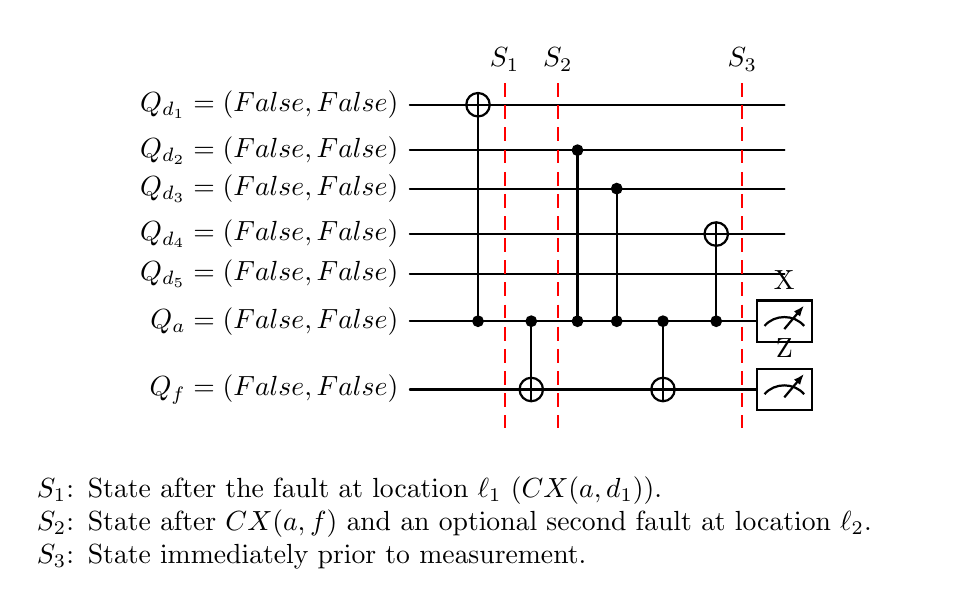
\begin{tikzpicture}

\node (circ) {
\begin{quantikz}[
row sep=0.34cm,
column sep=0.35cm,
wire types={q,q,q,q,q,q,q}
]
\lstick{$Q_{d_1}= (False,False)$} & \qw  & \targ{} \slice{$S_1$} & \qw \slice{$S_2$}& \qw & \qw & \qw & \qw \slice{$S_3$} & \qw \\
\lstick{$Q_{d_2}= (False,False)$} & \qw              & \qw                   & \qw & \ctrl{4} & \qw & \qw & \qw & \qw \\
\lstick{$Q_{d_3}= (False,False)$} & \qw              & \qw                   & \qw & \qw & \ctrl{3} & \qw & \qw & \qw \\
\lstick{$Q_{d_4}= (False,False)$} & \qw              & \qw                   & \qw & \qw & \qw & \qw & \targ{} & \qw \\
\lstick{$Q_{d_5}= (False,False)$} & \qw              & \qw                   & \qw & \qw & \qw & \qw & \qw & \qw \\
\lstick{$Q_{a}= (False,False)$}   & \qw              & \ctrl{-5}             & \ctrl{1} & \control{} & \control{} & \ctrl{1} & \ctrl{-2} & \meter{$X$} \\
\lstick{$Q_{f}= (False,False)$}   & \qw              & \qw                   & \targ{} & \qw & \qw & \targ{} & \qw & \meter{$Z$}
\end{quantikz}
};

\node[
below=0.35cm of circ,
align=left,
text width=0.92\textwidth
] {
$S_1$: State after the fault at location $\ell_1$ ($CX(a,d_1)$).\\
$S_2$: State after $CX(a,f)$ and an optional second fault at location $\ell_2$.\\
$S_3$: State immediately prior to measurement.
};

\end{tikzpicture}
\end{adjustbox}
\caption{Symbolic fault propagation on the flagged $XZZXI$ extraction circuit. Slices $S_1, S_2, S_3$ mark intermediate symbolic states referred to in the text.}
\label{fig:fault-propagation-circuit}
\end{figure}

At $S_1$, a fault at location $\ell_1$ (the first $CX$ gate) inserts Boolean fault variables $(x_{\ell_1,a}, z_{\ell_1,a}, x_{\ell_1,d_1}, z_{\ell_1,d_1})$ into the affected qubits:
\[
Q_a(\mathcal{F})=(x_{\ell_1,a},z_{\ell_1,a}), \qquad Q_{d_1}(\mathcal{F})=(x_{\ell_1,d_1},z_{\ell_1,d_1}).
\]

Next, passing through $CX(a,f)$ propagates $x_{\ell_1,a}$ to qubit $f$. If a second fault occurs at location $\ell_2$, its variables accumulate by XOR. As shown at slice $S_2$:
\[
Q_a(\mathcal{F}) = (x_{\ell_1,a}\oplus x_{\ell_2,a},\, z_{\ell_1,a}\oplus z_{\ell_2,a}), \qquad Q_f(\mathcal{F}) = (x_{\ell_1,a}\oplus x_{\ell_2,f},\, z_{\ell_2,f}).
\]
This illustrates the two operations used throughout symbolic Pauli execution: gates transform existing symbolic Pauli labels according to propagation rules, while faults at later locations contribute additional Boolean variables that accumulate via XOR.

% Continuing propagation through all gates yields the final pre-measurement state at slice $S_3$. The recorded outcomes for $X$-basis measured syndrome qubit $a$ and $Z$-basis measured flag qubit $f$ are given by:
% \[
% m_1(F) = Q_{a,z}(F), \qquad f_1(F) = Q_{f,x}(F).
% \]
% In general, measuring qubit $q$ in the $Z$-basis yields outcome $R_q(F)=Q_{q,x}(F)$, whereas an $X$-basis measurement yields $R_q(F)=Q_{q,z}(F)$. Each recorded outcome is thus a Boolean formula over the fault variables.

% The measurement record $m_\pi(F) = \bigl(R_1(F),\ldots,R_r(F)\bigr)$ collects all outcomes along path $\pi$. Equality between two records is encoded bitwise as:
% \[
% m_\pi(F_1) = m_\pi(F_2) \quad\equiv\quad \bigwedge_{j=1}^r \bigl(R_j(F_1)\leftrightarrow R_j(F_2)\bigr).
% \]

Continuing propagation through all gates yields the final pre-measurement state at slice $S_3$. In general, measuring a qubit $q$ extracts the Pauli component that anti-commutes with the measurement basis: an $X$-basis measurement yields $Q_{q,z}(\mathcal{F})$, while a $Z$-basis measurement yields $Q_{q,x}(\mathcal{F})$.

Thus, the recorded outcomes for syndrome qubit $a$ ($X$-basis) and flag qubit $f$ ($Z$-basis) are:
\[
m_1(\mathcal{F}) = Q_{a,z}(\mathcal{F}), \qquad f_1(\mathcal{F}) = Q_{f,x}(\mathcal{F}).
\]
Each recorded outcome is a Boolean formula over the fault variables.

The full measurement record $m_\pi(\mathcal{F}) = \bigl(R_1(\mathcal{F}), \ldots, R_r(\mathcal{F})\bigr)$ collects all $r$ syndrome and flag outcomes along path $\pi$ (where $R_j$ denotes the $j$-th recorded bit, e.g., $R_1 = m_1, R_2 = f_1$). Bitwise equality between two records is encoded as:
\[
m_\pi(\mathcal{F}_1) = m_\pi(\mathcal{F}_2) \quad\equiv\quad \bigwedge_{j=1}^r \bigl(R_j(\mathcal{F}_1)\leftrightarrow R_j(\mathcal{F}_2)\bigr).
\]

Finally, the same recorded syndrome and flag outcomes are substituted into the
branch guards of the control flow to form the path condition. For example,
suppose the terminating path $\pi$ first takes a branch guarded by
$m_1=0\land f_1=0$ and then a branch guarded by $m_2=1\lor f_2=1$. If symbolic
execution produces the recorded syndrome and flag outcomes
$m_1(\mathcal{F}),f_1(\mathcal{F}),m_2(\mathcal{F}),f_2(\mathcal{F})$, then the corresponding path condition is
\[
\Phi_\pi(\mathcal{F})
=
\neg m_1(\mathcal{F})
\land
\neg f_1(\mathcal{F})
\land
\bigl(m_2(\mathcal{F})\lor f_2(\mathcal{F})\bigr)
\land \cdots ,
\]
where the remaining conjuncts come from the later branch guards along $\pi$.
Thus, $\Phi_\pi(\mathcal{F})$ is obtained by substituting the symbolic recorded outcomes
into all branch guards along the terminating path and conjoining the resulting
formulas.

At this point, for every terminating path $\pi$ and fault assignment $\mathcal{F}$, we
have Boolean encodings of the three quantities used by the verification
queries: the path condition $\Phi_\pi(\mathcal{F})$, the residual data error
$E_\pi(\mathcal{F})$, and the measurement record $m_\pi(\mathcal{F})$.

\subsubsection{FTEC Check}
\label{subsec:ftec-check}

We first present the SAT formula for checking the condition in
Thm.~\ref{thm:mains}. This check is applied after the verifier has
established that the input protocol is valid in the sense of
Def.~\ref{def:protocol-validity}. As in Thm.~\ref{thm:mains}, we ignore
global phases and write the relative Pauli error as the product of the two
residual data errors.

For each terminating path $\pi$, the verifier searches for two fault
assignments $\mathcal{F}_1$ and $\mathcal{F}_2$ such that both executions follow $\pi$, both contain
at most $t$ faults, and both produce the same measurement record, but their
residual data errors violate the quantum error correction condition. The SAT
formula is

\begin{equation}
\begin{aligned}
\Psi^{\mathrm{FTEC}}_\pi
:=
\exists \mathcal{F}_1,\mathcal{F}_2.\quad
&
\Phi_\pi(\mathcal{F}_1)
\land
\Phi_\pi(\mathcal{F}_2)
\\
&\land\ \mathrm{wt}(\mathcal{F}_1)\le t
\land
\mathrm{wt}(\mathcal{F}_2)\le t
\\
&\land\ m_\pi(\mathcal{F}_1)=m_\pi(\mathcal{F}_2)
\\
&\land\ E_\pi(\mathcal{F}_1)\cdot E_\pi(\mathcal{F}_2)
\in N(\cS)\setminus\mathcal S .
\end{aligned}
\end{equation}

The first line requires both fault assignments to produce executions that
follow the terminating path $\pi$. The second line enforces the fault bound.
The third line requires the two executions to have the same measurement record.
The last line requires the two residual data errors to violate the quantum
error correction condition, since their product is a nontrivial logical
operator.

Thus, if $\Psi^{\mathrm{FTEC}}_\pi$ is satisfiable, the satisfying assignment
gives a concrete counterexample to the condition in
Thm.~\ref{thm:mains}. If $\Psi^{\mathrm{FTEC}}_\pi$ is unsatisfiable for
every terminating path $\pi$, then no such counterexample exists within the
fault bound. For a valid protocol, Thm.~\ref{thm:mains} implies that this
is equivalent to $\Pi$ satisfying FTEC.

It remains to encode the last conjunct of $\Psi^{\mathrm{FTEC}}_\pi$. Let

$
Q=E_\pi(\mathcal{F}_1) \cdot E_\pi(\mathcal{F}_2).
$
In the binary Pauli representation, $Q$ is obtained by XORing the two residual
data-error vectors. The condition
$
Q\in N(\mathcal S)\setminus\mathcal S
$
is encoded as the conjunction of normalizer membership and stabilizer
nonmembership.

Normalizer membership means that $Q$ commutes with every stabilizer generator
$G_j$. If
$
Q=(Q_{1,x},Q_{1,z},\ldots,Q_{n,x},Q_{n,z}),
$
then this is encoded by

\begin{equation} \label{eq:Normalize-membership}
    \begin{aligned}
       \mathrm{Norm}(Q,\mathcal{S}) =  \bigwedge_j
\left(
\bigoplus_{i=1}^n
\left(
Q_{i,x} \land G_{j,i,z}
\right)
\oplus
\left(
Q_{i,z} \land G_{j,i,x}
\right)
=0
\right).
    \end{aligned}
\end{equation}



Stabilizer nonmembership is encoded using a fixed set of logical Pauli operators
$
\mathcal{L} = L_1,\ldots,L_{2k},
$
precomputed from the stabilizer generators of the code.
Since the previous constraint already enforces $Q\in N(\mathcal S)$, the
condition $Q\notin\mathcal S$ is equivalent to saying that $Q$ has nontrivial
logical action. Equivalently, $Q$ must anticommute with at least one logical
Pauli generator. Thus the verifier encodes stabilizer nonmembership by

\begin{equation} \label{eq:stabiizer-nonmembership}
    \begin{aligned}
       \mathrm{Stab_{\mathrm{non}}}(Q, \mathcal{L}) = \bigvee_{h=1}^{2k}
\left(
\bigoplus_{i=1}^n
\left(
Q_{i,x} \land L_{h,i,z}
\right)
\oplus
\left(
Q_{i,z} \land L_{h,i,x}
\right)
=1
\right).
    \end{aligned}
\end{equation}

\bw{add equation  number and name of member for later will use in minimum weight checking }

Together, the normalizer-membership constraint and the logical-anticommutation
constraint encode
$
Q\in N(\mathcal S)\setminus\mathcal S.
$
Therefore $\Psi^{\mathrm{FTEC}}_\pi$ is a SAT query whose satisfying
assignments are exactly the counterexamples to the condition in
Thm.~\ref{thm:mains} on the path $\pi$.



\subsubsection{Check for Condition~(1) of Def.~\ref{def:control-flow-validity} used in Thm.~\ref{thm:mains}}
\label{subsec:cf-validity-condition1}

We next describe the SAT check for the assumption of Condition~(1) in Def.~\ref{def:control-flow-validity}, as required by Thm.~\ref{thm:mains}. We must check that if a path satisfies Condition~(1), any executions that produce the same measurement record leave residual data errors with the same ideal syndrome. Therefore, the verifier searches for a counterexample: two executions that follow the same terminating path and produce the same measurement record, but whose residual data errors have different ideal syndromes.

For each terminating path $\pi$ intended to satisfy Condition (1), the verifier
checks satisfiability of the formula
\begin{equation}
\begin{aligned}
\Psi^{\mathrm{CF1}}_\pi
:=
\exists \mathcal{F}_1,\mathcal{F}_2.\quad
&
\Phi_\pi(\mathcal{F}_1)
\land
\Phi_\pi(\mathcal{F}_2)
\\
&\land\ \mathrm{wt}(\mathcal{F}_1)\le t
\land
\mathrm{wt}(\mathcal{F}_2)\le t
\\
&\land\ m_\pi(\mathcal{F}_1)=m_\pi(\mathcal{F}_2)
\\
&\land\ \mathrm{syn}(E_\pi(\mathcal{F}_1))
\ne
\mathrm{syn}(E_\pi(\mathcal{F}_2)).
\end{aligned}
\end{equation}

The first two lines restrict the two fault assignments to executions that
follow the same terminating path and satisfy the fault bound. The third line
requires the two executions to have the same measurement record. The last line
requires their residual data errors to have different ideal syndromes.

The ideal syndrome is computed from the binary Pauli representation by the
usual symplectic inner product with the stabilizer generators. For a data error
$
E=(E_{1,x},E_{1,z},\ldots,E_{n,x},E_{n,z}),
$
the syndrome bit with respect to a stabilizer generator $G_j$ is

\[
\mathrm{syn}_j(E) = \bigoplus_{i=1}^n \bigl( (E_{i,x} \land G_{j,i,z}) \oplus (E_{i,z} \land G_{j,i,x}) \bigr).
\]
Thus the inequality of 
$
\mathrm{syn}(E_\pi(\mathcal{F}_1))
$ and $
\mathrm{syn}(E_\pi(\mathcal{F}_2))
$
is encoded as
\[
\bigvee_j
\left(
\mathrm{syn}_j(E_\pi(\mathcal{F}_1))
\oplus
\mathrm{syn}_j(E_\pi(\mathcal{F}_2))
\right).
\]

If $\Psi^{\mathrm{CF1}}_\pi$ is satisfiable, then the same measurement record
can correspond to two different ideal syndromes, so Condition (1) of
Def.~\ref{def:control-flow-validity} fails on $\pi$. If the formula is
unsatisfiable, then the measurement record uniquely determines the ideal
syndrome for all executions on $\pi$ within the fault bound.

\subsubsection{Control-Flow Validity: Condition (3)}
\label{subsec:cf-validity-condition3}

We next describe the SAT check for Condition (3) of
Def.~\ref{def:control-flow-validity}. This condition applies to terminating
paths for which the decoder applies the trivial correction. Therefore, given an input error $E_{in}$ with $wt(E)=r  $ and  every
fault event involving $r+ w\le t$ faults must already leave a residual data error
whose $ \mathrm{wt}_{\mathrm{min}}$ is at most $w$.

For each terminating path $\pi$ intended to satisfy Condition (3), and for each
$w=0,\ldots,t$, the verifier searches for a fault assignment that violates this
requirement:
\yfc{Please check the quantification of the input error and the combined
input-error and circuit-fault budget in the following formula.}
\yfc{The dependence of the residual error, path condition, and measurement
record on the input error is unclear in the current notation. Please check.}
\begin{equation}
\begin{aligned}
\Psi^{\mathrm{CF3}}_{\pi,w}
:=
\exists \mathcal{F}.\quad
&
\Phi_\pi(\mathcal{F})
\\
& \land\ \mathrm{wt}_(\mathcal{F}_{in}) =r
\\
&\land\ \mathrm{wt}(\mathcal{F}_{circ})=w
\\
&\land\ \mathrm{wt}_{\min}(E_\pi(\mathcal{F}))> w  .
\end{aligned}
\end{equation}
The first line requires the fault assignment to produce an execution that
follows the terminating path $\pi$. The second line fixes the number of faults
to be $w$. The last line requires the residual data error to have minimum
weight greater than $w$, even after multiplying by stabilizers.

\textcolor{blue}{Recall from Eq.~(\ref{eq:wt_min}) that 
$ \mathrm{wt}_{\min}(E) = \min_{S\in\mathcal{S}}\mathrm{wt}(E\cdot S). $ 
To encode the condition $\mathrm{wt}_{\min}(E_\pi(\mathcal{F})) > w$, we must assert that there exists no Pauli string $P$ of weight $\mathrm{wt}(P) \leq w$ such that $E_\pi(\mathcal{F})\cdot P \in \mathcal{S}$. A Pauli string belongs to the stabilizer group if it commutes with all stabilizer generators and logical operators. This can be formulated using the normalizer-membership (Eq.~\ref{eq:Normalize-membership}) and stabilizer-nonmembership (Eq.~\ref{eq:stabiizer-nonmembership}) constraints:}

\yfc{Please check the scope of the conjunction and disjunction
in the following minimum-weight encoding.}
\begin{equation} \label{eq:minimum-weight}
    \begin{aligned}
      \mathrm{wt}_{\min}(E_\pi(\mathcal{F}))>w \ =   \bigwedge_{P : \mathrm{wt}(P) \leq w } \neg  \mathrm{Norm}(P \cdot E_\pi(\mathcal{F}), \mathcal{S}) \lor \mathrm{Stab}_{\mathrm{non}}(P \cdot E_\pi(\mathcal{F}), \mathcal{L}) 
    \end{aligned}
\end{equation}



% Recall from Eq.~(\ref{eq:wt_min}) that $
% \mathrm{wt}_{\min}(E)
% =
% \min_{S\in\mathcal S}\mathrm{wt}(E\cdot S).
% $
% To encode $\mathrm{wt}_{\min}(E_\pi(\mathcal{F}))>w$, the verifier explicitly ranges over
% all stabilizer representatives. Let
% $
% \mathcal S=\langle G_1,\ldots,G_{n-k}\rangle .
% $
% % For each coefficient vector
% % $c=(c_1,\ldots,c_{n-k})\in\{0,1\}^{n-k}$, define the stabilizer representative
% % \[
% % S(c)=\prod_{j=1}^{n-k}G_j^{c_j}.
% % \]
% % In the binary Pauli representation, the $i$-th qubit component of
% % $E_\pi(F) \cdot S(c)$ is
% % \[
% % \bigl(
% % E_{i,x}(F)\oplus S_i^x(c),
% % \;
% % E_{i,z}(F)\oplus S_i^z(c)
% % \bigr),
% % \]
% % where
% % $
% % S_i^x(c)=\bigoplus_{j=1}^{n-k} c_jG_{j,i,x},
% % \qquad
% % S_i^z(c)=\bigoplus_{j=1}^{n-k} c_jG_{j,i,z}.
% % $


% % The $i$-th qubit contributes one to the weight of $E_\pi(F)S(c)$ exactly when
% % the Pauli operator on that qubit is not the identity. This is represented by
% % the Boolean variable
% % \[
% % b_i(c,F)
% % =
% % \bigl(E_{i,x}(F)\oplus S_i^x(c)\bigr)
% % \vee
% % \bigl(E_{i,z}(F)\oplus S_i^z(c)\bigr).
% % \]
% \

% For each coefficient vector $c=(c_1,\ldots,c_{n-k})\in\{0,1\}^{n-k}$, the stabilizer representative $S(c)=\prod_{j=1}^{n-k}G_j^{c_j}$ has binary components $S_i^x(c)=\bigoplus_{j=1}^{n-k} c_j \land G_{j,i,x}$ and $S_i^z(c)=\bigoplus_{j=1}^{n-k} c_j \land G_{j,i,z}$. 

% The $i$-th qubit component of $E_\pi(\mathcal{F}) \cdot S(c)$ is $\bigl(E_{i,x}(\mathcal{F})\oplus S_i^x(c),\, E_{i,z}(\mathcal{F})\oplus S_i^z(c)\bigr)$, and its non-identity support bit is given by:
% $
% b_i(c,\mathcal{F}) = \bigl(E_{i,x}(\mathcal{F})\oplus S_i^x(c)\bigr) \vee \bigl(E_{i,z}(\mathcal{F})\oplus S_i^z(c)\bigr).
% $

% Therefore the condition
% $
% \mathrm{wt}(E_\pi(\mathcal{F}) \cdot S(c))>w $
% is encoded as the cardinality constraint
% $
% \sum_{i=1}^n b_i(c,\mathcal{F})>w .
% $
% Finally,
% $
% \mathrm{wt}_{\min}(E_\pi(\mathcal{F}))>w
% $
% is encoded by requiring this constraint for every
% $c\in\{0,1\}^{n-k}$:
% \begin{equation}
% \label{eq:weight-greater-than}
% \begin{aligned}
% \bigwedge_{c\in\{0,1\}^{n-k}}
% \left(
% \sum_{i=1}^n b_i(c,\mathcal{F})>w
% \right).
% \end{aligned}
% \end{equation}


% \begin{example}
% Suppose the code has three data qubits and one stabilizer generator $G_1=ZZI$. In the binary Pauli representation, $G_1=((0,1),(0,1),(0,0))$. Let the symbolic residual data error be $E_\pi(\mathcal{F})=\bigl((E_{1,x},E_{1,z}),(E_{2,x},E_{2,z}),(E_{3,x},E_{3,z})\bigr)$. There is one stabilizer coefficient $c_1\in\{0,1\}$. The stabilizer representative selected by $c_1$ has binary components
% \[
% S_1^x(c_1)=0,\; S_1^z(c_1)=c_1; \qquad 
% S_2^x(c_1)=0,\; S_2^z(c_1)=c_1; \qquad 
% S_3^x(c_1)=0,\; S_3^z(c_1)=0.
% \]
% Therefore the support bits of $E_\pi(\mathcal{F})S(c_1)$ are
% \[
% b_1(c_1,\mathcal{F}) = E_{1,x} \vee (E_{1,z}\oplus c_1), \qquad
% b_2(c_1,\mathcal{F}) = E_{2,x} \vee (E_{2,z}\oplus c_1), \qquad
% b_3(c_1,\mathcal{F}) = E_{3,x} \vee E_{3,z}.
% \]
% Thus the condition that this representative has weight greater than $w$ is
% \[
% b_1(c_1,\mathcal{F})+b_2(c_1,\mathcal{F})+b_3(c_1,\mathcal{F})>w.
% \]
% To encode $\mathrm{wt}_{\min}(E_\pi(\mathcal{F}))>w$, the verifier requires this constraint for both choices of $c_1$:
% \[
% \bigl(b_1(0,\mathcal{F})+b_2(0,\mathcal{F})+b_3(0,\mathcal{F})>w\bigr) \land \bigl(b_1(1,\mathcal{F})+b_2(1,\mathcal{F})+b_3(1,\mathcal{F})>w\bigr).
% \]
% For $c_1=0$, this checks the weight of $E_\pi(\mathcal{F})$ itself. For $c_1=1$, this checks the weight after multiplying by the stabilizer $ZZI$.\qed
% \end{example}


If $\Psi^{\mathrm{CF3}}_{\pi,w}$ is satisfiable for some $w$, then there is a
$w$-fault execution on $\pi$ whose residual data error has minimum  weight larger
than $w$, so Condition (3) of Def.~\ref{def:control-flow-validity} fails on
$\pi$. If the formula is unsatisfiable for every $w=0,\ldots,t$, then
Condition (3) holds on $\pi$.

\subsubsection{$(t-w)$-Flag-Condition Check}
\label{subsec:tw-flag-condition-check}

We now describe the SAT check for the flag-condition requirement in
Def.~\ref{def:protocol-validity}. This check is applied only to terminating
paths satisfying Condition (2) of Def.~\ref{def:control-flow-validity}. For
such a path, the direct inspection used in the control-flow validity check
determines the number $w$ of detected faults on the path. The protocol validity
condition then requires the full syndrome extraction circuit used in the
repeated-syndrome suffix to satisfy the $(t-w)$-flag condition.

Let $C$ be this full syndrome extraction circuit, and let $F_C$ be the
set of flag qubits in $C$. For a fault assignment $\mathcal{F}$ on $C$, symbolic Pauli
propagation produces a residual data error $E_C(\mathcal{F})$ and, for each flag qubit
$q\in\mathcal F_C$, a recorded flag outcome $f_q(\mathcal{F})$. For each
$r=1,\ldots,t-w$, the verifier searches for an $r$-fault execution of $C$ that
raises no flag but leaves a residual data error whose $\mathrm{wt}_{\mathrm{min}}$ is larger
than $r$:
\begin{equation}
\begin{aligned}
\Psi^{\mathrm{flag}}_{C,r}
:=
\exists \mathcal{F}.\quad
&
\mathrm{wt}(\mathcal{F})=r
\\
&\land\ \bigwedge_{q\in\mathcal F_C}\neg f_q(\mathcal{F})
\\
&\land\ \mathrm{wt}_{\min}(E_C(\mathcal{F}))>r .
\end{aligned}
\end{equation}
The first line fixes the number of faults in the circuit to be $r$. The second
line requires that no flag qubit is raised. The last line requires the induced
residual data error to have $\mathrm{wt}_{\mathrm{min}}$ larger than $r$.

As in the Condition (3) check, the constraint
$\mathrm{wt}_{\min}(E_C(\mathcal{F}))>r$ is encoded using Eq.~\eqref{eq:weight-greater-than} with $w$ replaced by $r$.
\yfc{Please check this equation reference:
the label eq:weight-greater-than is currently commented out.}
In the binary Pauli representation, this is implemented by XORing the binary
vector of $E_C(\mathcal{F})$ with the selected stabilizer representative and applying a
cardinality constraint to the resulting support.

If $\Psi^{\mathrm{flag}}_{C,r}$ is satisfiable for some $r\le t-w$, then the
circuit violates the required $(t-w)$-flag condition: there is an unflagged
$r$-fault execution whose residual data error is not stabilizer-equivalent to
any Pauli error of weight at most $r$. If the formula is unsatisfiable for every
$r=1,\ldots,t-w$, then the circuit satisfies the required $(t-w)$-flag
condition.

\subsubsection{Circuit Correctness Check}
\label{subsec:circuit-correctness-check}

The first part of the circuit validity check verifies
the correctness condition in
Def.~\ref{def:syndrome-extraction-correct}.
This check is performed for each syndrome extraction
circuit in the protocol and must hold for every
possible input Pauli error on the data block.

Let $\cC$ be a circuit intended to measure
Pauli strings $\{P_i\}_{i=1}^{m}$.
The verifier symbolically propagates an input
Pauli error $E_{\mathrm{in}}$ on the data qubits
through $\cC$ without circuit faults.
Let $E_{\mathrm{out}}$ be the resulting data error,
and let $E_{\mathrm{anc}}$ be the propagated
ancilla error.

For each designated syndrome ancilla $i$, define
\[
    R_i(E_{\mathrm{in}})
    =E_{\mathrm{anc}}\odot A_i,
\]
where $A_i$ is its measurement observable.
Thus, $R_i(E_{\mathrm{in}})$ represents the
measurement-bit flip induced by the input Pauli
error relative to the fault-free reference outcome.

The verifier checks whether there exists an input
error for which either the propagated data error
is not stabilizer-equivalent to the input error
or some syndrome parity disagrees with the
ideal one:
\begin{equation}
\begin{aligned}
\Psi^{\mathrm{corr}}_{\cC}
:=
\exists E_{\mathrm{in}}.\;
\Bigl(
E_{\mathrm{out}}\not\sim E_{\mathrm{in}}
\;\vee\;
\bigvee_{i=1}^{m}
R_i(E_{\mathrm{in}})
\neq
E_{\mathrm{in}}\odot P_i
\Bigr).
\end{aligned}
\end{equation}
Here $\odot$ denotes the binary symplectic
product from Eq.~\ref{eq:symp_ip}, and $\sim$
denotes equivalence up to a data stabilizer
and Pauli phase which can be check by normalizer membership Eq. ~\ref{eq:Normalize-membership} and stabilizer nonmembership Eq. ~\ref{eq:stabiizer-nonmembership}.

If $\Psi^{\mathrm{corr}}_{\cC}$ is satisfiable,
the satisfying assignment gives an input
Pauli error witnessing that $\cC$ is not
correct. If it is unsatisfiable, then
$\cC$ satisfies
Def.~\ref{def:syndrome-extraction-correct}.

This check constrains only the designated
syndrome ancillas; no syndrome correctness
condition is imposed on the remaining ancillas.
Their measurement determinism is verified
separately.
\subsection{Simulation and Direct-Inspection Checks}
\label{subsec:simulation-direct-checks}

The SAT checks above verify properties naturally
expressed as the absence of a counterexample.
The remaining checks use different mechanisms.
The second part of circuit validity verification
uses fault-free stabilizer-tableau simulation,
while Condition (2) of
Def.~\ref{def:control-flow-validity}
is checked directly from the structure of
the terminating path.

\subsubsection{Circuit Determinism Check}
\label{subsec:circuit-validity-check}

The second part of the circuit validity check
verifies the determinism condition in
Def.~\ref{def:syndrome-extraction-deterministic}.
Unlike the correctness check, this check
considers all ancilla measurements, including
those not designated for syndrome extraction.

Theorem~\ref{thm:syndrome-extraction-valid}
establishes that, once circuit correctness
is verified, circuit validity is equivalent
to joint stabilizer preservation and logical
preservation. Both conditions can be checked
using stabilizer-tableau simulation.

The verifier propagates the joint data-ancilla
stabilizer generators through the Clifford
gates and checks whether the resulting signed
stabilizer group equals the initial joint
stabilizer group. It also verifies that each
logical Pauli generator is preserved up to
an element of the joint stabilizer group.

Table~\ref{tab:stabilizer-evolution} illustrates
the stabilizer propagation underlying this
check by tracking the evolution of the joint
data-ancilla stabilizer generators through
the Clifford gates. The verifier performs
the same computation using stabilizer-tableau
simulation.

Joint stabilizer preservation ensures that
all ancilla measurements have the intended
deterministic outcomes in the error-free
execution, while logical preservation ensures
that the encoded logical state remains
unchanged. Since Clifford circuits propagate
Pauli errors to Pauli errors, an arbitrary
input data Pauli error can only change the
ancilla measurement outcomes by fixed
commutation signs. Consequently, all ancilla
outcomes are determined independently of
the encoded state and can serve as well-defined
entries in the measurement record.

If either preservation condition fails,
the circuit does not satisfy the validity
characterization in
Theorem~\ref{thm:syndrome-extraction-valid}
and is rejected by the verifier.
\subsubsection{Control-Flow Validity: Condition (2)}
\label{subsec:cf-validity-condition2}

Condition (2) of Def.~\ref{def:control-flow-validity} is checked by direct
inspection of terminating paths. This condition applies to paths that terminate
after a repeated full-syndrome suffix. For each such path $\pi$, the verifier
infers a detected-fault lower bound $w$ from the preceding measurement
record using the counting rule of~\cite[Sections~2.2 and~3.1]{CB18}.
In particular, when comparing consecutive unflagged full-syndrome
rounds, a syndrome change increments the counter by one only if the
preceding comparison did not increment it.
It then checks that the terminating suffix contains $t-w+1$ consecutive full
syndrome extraction rounds whose recorded syndrome outcomes are required by the
branch guards to be identical, and whose flag outcomes are required to be zero.

This check is structural: it does not search over fault assignments. It only
verifies that the control flow has the form required by Condition (2). The
soundness of using the repeated syndrome value is supplied by the validity of
the full syndrome extraction circuits and by the $(t-w)$-flag-condition check
from Section~\ref{subsec:tw-flag-condition-check}.
\subsection{Overall Algorithm}
\label{subsec:overall-algorithm}

Algorithm~\ref{alg:ftec-verification} summarizes the verification procedure. Although the previous subsections present the SAT-based checks first, the algorithm first establishes protocol validity, because Thm.~\ref{thm:mains} applies only to valid protocols. If the protocol is invalid, it returns \textsc{NotValid}. If valid, the algorithm then checks the condition in Thm.~\ref{thm:mains} on every terminating path and returns either \textsc{NotFTEC} or \textsc{FTEC}.

\begin{algorithm}[t]

\DontPrintSemicolon
\SetAlgoLined
\SetAlgoNoEnd
\caption{Verification of a flagged error correction protocol}
\label{alg:ftec-verification}
\KwIn{Stabilizer code $\mathcal Q$, flagged protocol $\Pi$, fault bound $t$}
\KwOut{\textsc{NotValid}, \textsc{NotFTEC}, or \textsc{FTEC}}

\ForEach{syndrome extraction circuit $C$ used in $\Pi$}{
    \lIf{\textsc{CircuitValidity}$(C)$ fails}{\Return \textsc{NotValid}}
}

\ForEach{terminating path $\pi\in \Pi$}{
    \lIf{\textsc{ControlFlowValidity}$(\pi,t)$ fails}{\Return \textsc{NotValid}}
    
    \If{$\pi$ satisfies Condition (2) with detected-fault count $w$}{
        \ForEach{full syndrome extraction circuit $C\in \pi$}{\lIf{\textsc{FlagCondition}$(C,t-w)$ fails}{\Return \textsc{NotValid}}}
    }
}

\ForEach{terminating path $\pi\in\Pi$}{
    \lIf{$\Psi^{\mathrm{FTEC}}_\pi$ is SAT}{\Return \textsc{NotFTEC}}
}

\Return \textsc{FTEC}
\end{algorithm}

The subroutines in Algorithm~\ref{alg:ftec-verification} refer to the checks
defined above. \textsc{CircuitValidity} checks
Def.~\ref{def:syndrome-extraction-valid} by stabilizer-tableau simulation.
\textsc{ControlFlowValidity} checks Def.~\ref{def:control-flow-validity} \footnote{The check of Condition (1) in Def. \ref{def:control-flow-validity} used in Thm. \ref{thm:mains} is also included here}: it
uses $\Psi^{\mathrm{CF1}}_\pi$ for Condition (1), direct inspection for
Condition (2), and $\Psi^{\mathrm{CF3}}_{\pi,w}$ for Condition (3). For a path
satisfying Condition (2), the detected-fault count $w$ returned by direct
inspection determines the parameter of the required
\textsc{FlagCondition}$(C,t-w)$ check. 
Note that, along the path $\pi$, we only need to check the flag condition for the
full syndrome extraction circuit as required by Def.~\ref{def:protocol-validity}(3).

\begin{theorem}[Verification correctness]
\label{thm:verification-correctness}
Algorithm~\ref{alg:ftec-verification} satisfies the following:
\begin{enumerate}
    \item If it returns \textsc{NotValid}, then $\Pi$ fails
    Def.~\ref{def:protocol-validity}.
    \item If it returns \textsc{NotFTEC}, then $\Pi$ is a valid protocol but
    does not satisfy FTEC.
    \item If it returns \textsc{FTEC}, then $\Pi$ is a valid protocol and
    satisfies FTEC.
\end{enumerate}
\end{theorem}

\begin{proof}
\yfc{Compress this proof to three sentences: failed validity checks yield
NotValid; a SAT witness yields NotFTEC by the characterization theorem;
validity plus UNSAT for every path yields FTEC. The current proof repeats
the algorithm and the previously defined counterexample semantics.}
If the algorithm returns \textsc{NotValid}, then one of the checks used to
establish Def.~\ref{def:protocol-validity} has failed: either a syndrome
extraction circuit fails Def.~\ref{def:syndrome-extraction-valid}, a
terminating path fails Def.~\ref{def:control-flow-validity}, or a required
$(t-w)$-flag condition fails. Hence $\Pi$ fails
Def.~\ref{def:protocol-validity}.

Suppose the algorithm reaches the FTEC-check loop. Then all protocol-validity
checks have passed, so $\Pi$ is a valid protocol in the sense of
Def.~\ref{def:protocol-validity}. If the algorithm returns \textsc{NotFTEC},
then $\Psi^{\mathrm{FTEC}}_\pi$ is satisfiable for some terminating path
$\pi$. Thus, there exist two executions within the fault bound that follow the
same terminating path, produce the same measurement record, and leave residual
data errors whose product lies in
$N(\mathcal S)\setminus\mathcal S$. This violates the condition in
Thm.~\ref{thm:mains}. Since $\Pi$ is valid, the theorem implies that
$\Pi$ does not satisfy FTEC.

Finally, if the algorithm returns \textsc{FTEC}, then all protocol-validity
checks have passed and every formula $\Psi^{\mathrm{FTEC}}_\pi$ is
unsatisfiable. Hence no two executions within the fault bound produce the same
measurement record while leaving residual data errors whose product lies in
$N(\mathcal S)\setminus\mathcal S$. Therefore the condition in
Thm.~\ref{thm:mains} holds. Since $\Pi$ is valid, the theorem implies
that $\Pi$ satisfies FTEC.
\end{proof}

\section{Related Work}

Recent works have made significant progress in verifying quantum error correction circuits using SAT solvers. For example, Chen et al.~\cite{chen2025verifying} employ symbolic execution to check if injected faults in quantum gadgets violate fault-tolerance conditions. Similarly, Huang et al.~\cite{10.1145/3729293} introduce Veri-QEC, a formal verification framework that translates Pauli errors into classical assertions solved by SAT solvers. 

However, applying these general methods to flagged syndrome extraction circuits creates a major bottleneck if an explicit decoder is not provided. In these frameworks, two distinct faults might produce the exact same syndrome. Without a predefined decoder to resolve this ambiguity, their tools cannot determine whether the post-recovery state will actually cause a logical error. 
Furthermore,  a residual error of weight greater than $t$ cannot by itself be used to determine correctability, since it
may be equivalent, up to a stabilizer, to a lower-weight error. 
This issue naturally arises in flagged protocols, where a single fault may propagate to a
high-weight data error.

Our work bypasses these limitations by adopting a specialized approach. By focusing strictly on flagged fault-tolerant error correction protocols, we completely eliminate the need for an explicit decoder during the verification process.
Rather than constructing a decoder and evaluating its performance, we establish a theorem that characterizes FTEC directly in terms of the residual-error sets associated with measurement records.
Beyond these theoretical guarantees, our framework demonstrates clear practical utility: by applying our method, we successfully identified previously unknown design flaws in published flagged error correction protocols.
\paragraph{Other automatic approaches for quantum circuit verification.}

Beyond quantum error correction, a variety of automated techniques have been developed for quantum circuit and program verification. Symbolic-execution-based approaches, such as SymQV~\cite{BauerMarquartLS23}, encode circuit semantics and verification conditions as SMT queries. Other works use automata-based representations of quantum states and symbolic gate execution~\cite{ChenCLLTY23,ChenCLLT23,abdulla2025verifying,autoq2,abdulla2026parameterized}, SMT array theories~\cite{chen2023theory}, or abstract interpretation~\cite{yu2021quantum,perdrix2008quantum} to reason about quantum programs.

These techniques have primarily been evaluated on functional correctness properties of quantum circuits and programs rather than fault-tolerance properties of quantum error-correction protocols. Nevertheless, many of the underlying ideas, such as symbolic execution, symbolic state representations, and automated constraint solving, appear potentially applicable to QECC verification as well. 
These techniques provide useful foundations for automated QECC verification, but their application to fault-tolerance properties involving fault propagation, stabilizer degeneracy, and recovery correctness requires additional structure.



Our work represents one step in this direction. By exploiting the structure of flagged syndrome-extraction protocols, we obtain a SAT-based verification procedure that avoids explicit decoder construction while still providing a complete correctness guarantee.


\section{Results}
\yfc{Please check how the FTEC queries reported for validity-failing
configurations relate to the final verdict of Algorithm~\ref{alg:ftec-verification}.
Please also check that the reported counterexamples use realizable executions
within the stated fault budget.}
Our experiments were conducted on a server running Ubuntu 22.04.3 LTS with an
AMD EPYC 7742 64-core processor (1.5\,GHz), 2\,TiB of RAM, and a 1\,TB SSD. We implemented our verification framework using Z3py to encode the constraints, which were subsequently transformed into DIMACS format for the CryptoMiniSat solver. CryptoMiniSat was chosen for its highly optimized performance on formulas containing massive XOR clauses. All tasks were executed without a time limit. 

% \begin{table}[!htbp]
% \centering

% % ==================== PART 1 ====================
% \scalebox{0.85}{% Applies the exact same scaling factor to both tables
% \scriptsize 
% \setlength{\tabcolsep}{4pt} 
% \begin{tabular}{l ccccccccc}
% \toprule
%  \multicolumn{10}{c}{\textbf{Protocol}} \\
% \midrule
% Code & $[[5,1,3]]$ & $[[5,1,3]]$ & $[[5,1,3]]$ & $[[5,1,3]]$ & $[[5,1,3]]$ & $[[5,1,3]]$ & $[[7,1,3]]$ & $[[7,1,3]]$ & $[[19,1,5]]$ \\
% Optimization & Low-depth & $[1,1,1,1]^{T}$ & $[2,2]$ & $[2,2]^{T}$ & $[2,2]^{T}$ fix$_2$ & Origin & Low-depth & Low-depth$_2$ & $[2,2,2,1,1,1]^{T}$ \\
% Protocol & [Bha23] & [LL25] & [LL25]  & [LL25]  & [LL25] & [RC18]  & [Bha23] & [Bha23] & [LL25] \\
% Total circuits & 14 & 2 & 2 & 2 & 2 & 6 & 4 & 14 & 2 \\
% Total paths & 13 & 2 & 2 & 2 & 2 & 5 & 4 & 19 & 4 \\
% \midrule
% \multicolumn{10}{c}{\textbf{Protocol Verification}} \\
% \midrule
% Syndrome extraction bugs (circuit) & 0 & 0 & 2 & 2 & 0 & 0 & 0 & 0 & 0 \\
% Control flow bugs (path) & 7 & 0 & 0 & 0 & 0 & 0 & 2 & 6 & 0 \\
% Flag bugs (circuit) & 0 & 0 & 0 & 0 & 0 & 0 & 0 & 0 & 0 \\
% \midrule
% \multicolumn{10}{l}{\textit{Stim}} \\
% Stim Runtime (s) & 0.607 & 0.085 & 0.088 & 0.087 & 0.088 & 0.203 & 0.163 & 0.548 & 0.159 \\
% Stim Peak Mem (MB) & 219.5 & 228.2 & 197.8 & 194.9 & 206.4 & 220.3 & 193.1 & 218.6 & 200.1 \\
% \midrule
% \multicolumn{10}{l}{\textit{SAT Solver}} \\
% Total Runtime (s) & 1.037 & 0.322 & 0.326 & 0.299 & 0.313 & 0.810 & 1.018 & 1.662 & 0.773 \\
% Peak Memory (MB) & 92.1 & 92.4 & 93.0 & 92.4 & 92.4 & 92.1 & 92.1 & 92.2 & 14914.4 \\
% Total SAT Calls & 30 & 5 & 5 & 5 & 5 & 15 & 11 & 44 & 7 \\
% Total SAT Time (s) & 0.177 & 0.108 & 0.090 & 0.050 & 0.104 & 0.121 & 0.094 & 0.266 & 806.32 \\
% \#Vars & 45--656 & 188--656 & 183--658 & 184--660 & 184--664 & 45--656 & 147--820 & 45--848 & 2082--5506178 \\
% \#Clauses & 352--4754 & 2053--4766 & 2049--4802 & 2049--4802 & 2049--4826 & 352--4756 & 1198--6008 & 340--6317 & 5484--146548287 \\
% \midrule
% \multicolumn{10}{c}{\textbf{FTEC}} \\
% \midrule
% FTEC (path) & 0 & 0 & 1 & 1 & 1 & 0 & 1 & 0 & 0 \\
% Time (s) & 0.351 & 0.091 & 0.088 & 0.085 & 0.096 & 0.192 & 0.143 & 0.155 & 0.262 \\
% Peak Mem (MB) & 85.4 & 88.0 & 90.0 & 90.0 & 71.0 & 87.0 & 87.8 & 87.6 & 144.3 \\
% SAT Calls & 13 & 2 & 2 & 2 & 2 & 5 & 4 & 19 & 4 \\
% Total SAT Time (s) & 0.145 & 0.065 & 0.027 & 0.057 & 0.058 & 0.079 & 0.052 & 0.207 & 2104.4 \\
% \#Vars & 278--626 & 366--626 & 374--624 & 376--624 & 461--776 & 348--626 & 397--774 & 274--803 & 2373--8973 \\
% \#Clauses & 2010--4576 & 2670--4588 & 2714--4620 & 2724--4620 & 3444--5798 & 2458--4578 & 2828--5742 & 1974--6033 & 20085--66716 \\
% \bottomrule
% \end{tabular}%
% }

% \vspace*{1.5em} % Adds a nice visual break between the two tables

% % ==================== PART 2 ====================
% \scalebox{0.85}{% Exactly the same scaling factor as Part 1
% \scriptsize 
% \setlength{\tabcolsep}{4pt}
% \begin{tabular}{l ccccccc}
% \toprule
%  \multicolumn{8}{c}{\textbf{Protocol}} \\
% \midrule
% Code & $[[19,1,5]]$ & $[[17,1,5]]$ & $[[17,1,5]]$ & $[[17,1,5]]$ & $[[17,1,5]]$ & $[[19,1,5]]$ & $[[25,1,5]]$ \\
% Optimization & $[1,1,1,\dots]^{T}$ & $[2,2,2,1,1]^{T}$ & $[1,1,1,1,1,\dots]^{T}$ & Par. flag & Seq. & Par. flag & Seq. \\
% Protocol & [LL25]  & [LL25]  & [LL25]  & [Du24]  & [CB18]  & [Du24]  & [CB18]  \\
% Total circuits & 2 & 2 & 2 & 2 & 2 & 2 & 2 \\
% Total paths & 4 & 4 & 4 & 21 & 21 & 21 & 21 \\
% \midrule
% \multicolumn{8}{c}{\textbf{Protocol Verification}} \\
% \midrule
% Syndrome extraction bugs (circuit) & 0 & 0 & 0 & 0 & 0 & 0 & 0 \\
% Control flow bugs (path) & 0 & 0 & 0 & 0 & 0 & 0 & 0 \\
% Flag bugs (circuit) & 0 & 0 & 0 & 1 & 0 & 1 & 0 \\
% \midrule
% \multicolumn{8}{l}{\textit{Stim}} \\
% Stim Runtime (s) & 0.170 & 0.258 & 0.168 & 0.144 & 0.148 & 0.154 & 0.186 \\
% Stim Peak Mem (MB) & 236.0 & 227.7 & 220.7 & 197.1 & 228.9 & 195.0 & 217.0 \\
% \midrule
% \multicolumn{8}{l}{\textit{SAT Solver}} \\
% Total Runtime (s) & 0.816 & 1097.36 & 1159.72 & 0.696 & 5.385 & 0.797 & 37.222 \\
% Peak Memory (MB) & 14916.4 & 8119.3 & 8126.8 & 391.6 & 224.6 & 202.7 & 183.1 \\
% Total SAT Calls & 7 & 7 & 7 & 37 & 36 & 36 & 37 \\
% Total SAT Time (s) & 794.70 & 1266.60 & 1406.90 & 17096.22 & 7614.65 & 49352.46 & 3146.30 \\
% \#Vars & 2088--5506171 & 5393--1377250 & 5321--1377246 & 2378--11697 & 5039--11889 & 1708--14317 & 4952--21105 \\
% \#Clauses & 5094--146548217 & 48159--27335500 & 47631--27335447 & 5825--122996 & 46654--120744 & 3664--119917 & 45073--153479 \\
% \midrule
% \multicolumn{8}{c}{\textbf{FTEC}} \\
% \midrule
% FTEC(path) & 0 & 0 & 0 & 3 & 0 & 0 & 0 \\
% Time (s) & 0.307 & 0.262 & 0.257 & 0.211 & 0.222 & 0.263 & 0.348 \\
% Peak Mem (MB) & 155.6 & 111.8 & 114.6 & 306.3 & 164.1 & 321.4 & 172.8 \\
% SAT Calls & 4 & 4 & 4 & 21 & 21 & 21 & 21 \\
% Total SAT Time (s) & 2312.0 & 1243.5 & 1562.3 & 123486.4 & 86124.3 & 151274.4 & 40477.4 \\
% \#Vars & 2362--8868 & 2051--7749 & 2041--7648 & 5466--11582 & 5494--11755 & 6586--14266 & 5372--11398 \\
% \#Clauses & 19960--66195 & 14410--57111 & 14304--56636 & 48370--122417 & 50906--120417 & 45341--119101 & 49264--123632 \\
% \bottomrule
% \end{tabular}%
% }
% \caption{Experimental results of the protocol verification and FTEC verification (Top: Part 1, Bottom: Part 2).}
% \label{tab:combined-results}

% \end{table}


% \begin{table}[!htbp]
% \centering

% % ==================== PART 1 ====================
% \scalebox{0.85}{% Applies the exact same scaling factor to both tables
% \scriptsize
% \setlength{\tabcolsep}{4pt}
% \begin{tabular}{l ccccccccc}
% \toprule
%  \multicolumn{10}{c}{\textbf{Protocol}} \\
% \midrule
% Code & $[[5,1,3]]$ & $[[5,1,3]]$ & $[[5,1,3]]$ & $[[5,1,3]]$ & $[[5,1,3]]$ & $[[5,1,3]]$ & $[[7,1,3]]$ & $[[7,1,3]]$ & $[[19,1,5]]$ \\
% Optimization & Low-depth & $[1,1,1,1]^{T}$ & $[2,2]$ & $[2,2]^{T}$ & $[2,2]^{T}$ fix$_2$ & Origin & Low-depth & Low-depth$_2$ & $[2,2,2,1,1,1]^{T}$ \\
% Protocol & [Bha23] & [LL25] & [LL25]  & [LL25]  & [LL25] & [RC18]  & [Bha23] & [Bha23] & [LL25] \\
% Total circuits & 14 & 2 & 2 & 2 & 2 & 6 & 4 & 14 & 2 \\
% Total paths & 13 & 2 & 2 & 2 & 2 & 5 & 4 & 19 & 4 \\
% \midrule
% \multicolumn{10}{c}{\textbf{Protocol Verification}} \\
% \midrule
% Syndrome extraction bugs (circuit) & 0 & 0 & 2 & 2 & 0 & 0 & 0 & 0 & 0 \\
% Control flow bugs (path) & 7 & 0 & 0 & 0 & 0 & 0 & 2 & 6 & 1 \\
% Flag bugs (circuit) & 0 & 0 & 0 & 0 & 0 & 0 & 0 & 0 & 0 \\
% \midrule
% \multicolumn{10}{l}{\textit{Stim}} \\
% Stim Runtime (s) & 0.607 & 0.085 & 0.088 & 0.087 & 0.088 & 0.203 & 0.163 & 0.548 & 0.159 \\
% Stim Peak Mem (MB) & 219.5 & 228.2 & 197.8 & 194.9 & 206.4 & 220.3 & 193.1 & 218.6 & 200.1 \\
% \midrule
% \multicolumn{10}{l}{\textit{SAT Solver}} \\
% Peak Memory (MB) & 92.1 & 92.4 & 93.0 & 92.4 & 92.4 & 92.1 & 100.2 & 92.2 & 34332.1 \\
% Total SAT Calls & 31 & 5 & 5 & 5 & 5 & 16 & 11 & 39 & 6 \\
% Total SAT Time (s) & 0.177 & 0.108 & 0.090 & 0.050 & 0.104 & 0.121 & 0.094 & 0.266 & 16109.1 \\
% Total CPU Time (s) & 9.2 & 3.9 & 3.9 & 3.9 & 4.0 & 4.9 & 5.9 & 14.3 & 25958.3 \\
% \#Vars & 45--615 & 188--615 & 183--625 & 184--627 & 184--623 & 45--615 & 147--763 & 45--793 & 6480--5506178 \\
% \#Clauses & 352--4551 & 2053--4563 & 2049--4623 & 2049--4623 & 2049--4623 & 352--4553 & 1198--5717 & 340--6317 & 53375--146548287 \\
% \midrule
% \multicolumn{10}{c}{\textbf{FTEC}} \\
% \midrule
% FTEC (path) & 0 & 0 & 1 & 1 & 1 & 0 & 1 & 0 & 0 \\
% Peak Mem (MB) & 85.4 & 88.0 & 90.0 & 90.0 & 71.0 & 87.0 & 87.8 & 87.6 & 144.3 \\
% SAT Calls & 13 & 2 & 2 & 2 & 2 & 5 & 4 & 19 & 4 \\
% Total SAT Time (s) & 0.145 & 0.065 & 0.027 & 0.057 & 0.058 & 0.079 & 0.052 & 0.207 & 2104.4 \\
% Total CPU Time (s) & 5.2 & 3.1 & 3.3 & 3.4 & 3.0 & 3.9 & 4.7 & 7.5 & 2131.4 \\
% \#Vars & 278--626 & 366--626 & 374--624 & 376--624 & 461--776 & 348--626 & 397--774 & 274--803 & 2373--8973 \\
% \#Clauses & 2010--4576 & 2670--4588 & 2714--4620 & 2724--4620 & 3444--5798 & 2458--4578 & 2828--5742 & 1974--6033 & 20085--66716 \\
% \bottomrule
% \end{tabular}%
% }

% \vspace*{1.5em} % Adds a nice visual break between the two tables

% % ==================== PART 2 ====================
% \scalebox{0.85}{% Exactly the same scaling factor as Part 1
% \scriptsize
% \setlength{\tabcolsep}{4pt}
% \begin{tabular}{l ccccccc}
% \toprule
%  \multicolumn{8}{c}{\textbf{Protocol}} \\
% \midrule
% Code & $[[19,1,5]]$ & $[[17,1,5]]$ & $[[17,1,5]]$ & $[[17,1,5]]$ & $[[17,1,5]]$ & $[[19,1,5]]$ & $[[25,1,5]]$ \\
% Optimization & $[1,1,1,\dots]^{T}$ & $[2,2,2,1,1]^{T}$ & $[1,1,1,1,1,\dots]^{T}$ & Par. flag & Seq. & Par. flag & Seq. \\
% Protocol & [LL25]  & [LL25]  & [LL25]  & [Du24]  & [CB18]  & [Du24]  & [CB18]  \\
% Total circuits & 2 & 2 & 2 & 2 & 2 & 2 & 2 \\
% Total paths & 4 & 4 & 4 & 21 & 21 & 21 & 21 \\
% \midrule
% \multicolumn{8}{c}{\textbf{Protocol Verification}} \\
% \midrule
% Syndrome extraction bugs (circuit) & 0 & 0 & 0 & 0 & 0 & 0 & 0 \\
% Control flow bugs (path) & 0 & 1 & 1 & 0 & 0 & 0 & 0 \\
% Flag bugs (circuit) & 0 & 0 & 0 & 1 & 0 & 1 & 0 \\
% \midrule
% \multicolumn{8}{l}{\textit{Stim}} \\
% Stim Runtime (s) & 0.170 & 0.258 & 0.168 & 0.144 & 0.148 & 0.154 & 0.186 \\
% Stim Peak Mem (MB) & 236.0 & 227.7 & 220.7 & 197.1 & 228.9 & 195.0 & 217.0 \\
% \midrule
% \multicolumn{8}{l}{\textit{SAT Solver}} \\
% Peak Memory (MB) & 34329.7 & 8119.3 & 17989.6 & 18004.0 & 18004.1 & 73989.4 & 162.1 \\
% Total SAT Calls & 6 & 6 & 6 & 18 & 18 & 18 & 18 \\
% Total SAT Time (s) & 24662.3 & 144.6 & 2491.0 & 17395.9 & 8891.3 & 50040.3 & 3146.30 \\
% Total CPU Time (s) & 34350.9 & 2203.6 & 4720.1 & 18638.7 & 10177.3 & 55473.0 & 3323.1 \\
% \#Vars & 6409--5506171 & 5390--2295123 & 5324--2295129 & 4918--1377144 & 5039--1377172 & 5925--5506042 & 4952--21105 \\
% \#Clauses & 53020--146548217 & 48101--39995851 & 47621--39995821 & 43363--27334792 & 46654--27335250 & 49992--146547428 & 45073--153479 \\
% \midrule
% \multicolumn{8}{c}{\textbf{FTEC}} \\
% \midrule
% FTEC(path) & 0 & 0 & 0 & 3 & 0 & 0 & 0 \\
% Peak Mem (MB) & 155.6 & 111.8 & 114.6 & 306.3 & 164.1 & 321.4 & 172.8 \\
% SAT Calls & 4 & 4 & 4 & 21 & 21 & 21 & 21 \\
% Total SAT Time (s) & 2312.0 & 1243.5 & 1562.3 & 123486.4 & 86124.3 & 151274.4 & 40477.4 \\
% Total CPU Time (s) & 2344.7 & 1265.1 & 1583.4 & 123713.2 & 86424.3 & 151579.6 & 40816.1 \\
% \#Vars & 2362--8868 & 2051--7749 & 2041--7648 & 5466--11582 & 5494--11755 & 6586--14266 & 5372--11398 \\
% \#Clauses & 19960--66195 & 14410--57111 & 14304--56636 & 48370--122417 & 50906--120417 & 45341--119101 & 49264--123632 \\
% \bottomrule
% \end{tabular}%
% }
% \caption{Experimental results of the protocol verification and FTEC verification (Top: Part 1, Bottom: Part 2). Total CPU Time differs from Total SAT Time by including symbolic execution and DIMACS export .}
% \label{tab:combined-results}

% \end{table}

\begin{table}[!htbp]
\centering

% ==================== PART 1 ====================
\scalebox{0.85}{% Applies the exact same scaling factor to both tables
\scriptsize
\setlength{\tabcolsep}{4pt}
\begin{tabular}{l ccccccccc}
\toprule
 \multicolumn{10}{c}{\textbf{Protocol}} \\
\midrule
Code & $[[5,1,3]]$ & $[[5,1,3]]$ & $[[5,1,3]]$ & $[[5,1,3]]$ & $[[5,1,3]]$ & $[[5,1,3]]$ & $[[7,1,3]]$ & $[[7,1,3]]$ & $[[19,1,5]]$ \\
Optimization & Low-depth & $[1,1,1,1]^{T}$ & $[2,2]$ & $[2,2]^{T}$ & $[2,2]^{T}$ fix$_2$ & Origin & Low-depth & Low-depth$_2$ & $[2,2,2,1,1,1]^{T}$ \\
Protocol & [Bha23] & [LL25] & [LL25]  & [LL25]  & [LL25] & [RC18]  & [Bha23] & [Bha23] & [LL25] \\
Total circuits & 14 & 2 & 2 & 2 & 2 & 6 & 4 & 14 & 2 \\
Total paths & 13 & 2 & 2 & 2 & 2 & 5 & 4 & 19 & 4 \\
\midrule
\multicolumn{10}{c}{\textbf{Protocol Verification}} \\
\midrule
Syndrome extraction bugs (circuit) & 0 & 0 & 2 & 2 & 0 & 0 & 0 & 0 & 0 \\
Control flow bugs (path) & 7 & 0 & 0 & 0 & 0 & 0 & 1 & 6 & 1 \\
Flag bugs (circuit) & 0 & 0 & 0 & 0 & 0 & 0 & 0 & 0 & 0 \\
\midrule
\multicolumn{10}{l}{\textit{Stim}} \\
Stim Runtime (s) & 0.523 & 0.086 & 0.085 & 0.083 & 0.088 & 0.203 & 0.143 & 0.382 & 0.152 \\
Stim Peak Mem (MB) & 212.1 & 223.8 & 197.4 & 215.0 & 203.3 & 199.3 & 236.5 & 204.4 & 198.8 \\
\midrule
\multicolumn{10}{l}{\textit{SAT Solver}} \\
Peak Memory (MB) & 91.6 & 98.5 & 91.6 & 100.0 & 99.7 & 99.9 & 100.2 & 90.7 & 101.4 \\
Total SAT Calls & 17 & 3 & 3 & 3 & 3 & 10 & 7 & 25 & 4 \\
Total SAT Time (s) & 4.850 & 0.927 & 0.931 & 0.968 & 0.965 & 2.071 & 2.099 & 8.228 & 32.8 \\
Total CPU Time (s) & 10.2 & 4.3 & 4.1 & 4.2 & 4.5 & 6.2 & 6.4 & 16.4 & 60.5 \\
\#Vars & 58--615 & 192--615 & 193--625 & 194--627 & 186--623 & 58--615 & 85--763 & 51--793 & 1104--8973 \\
\#Clauses & 312--4551 & 1369--4563 & 1385--4623 & 1385--4623 & 1345--4623 & 312--4553 & 524--5717 & 272--5999 & 8806--66744 \\
\midrule
\multicolumn{10}{c}{\textbf{FTEC}} \\
\midrule
FTEC (path) & 0 & 0 & 1 & 1 & 1 & 0 & 1 & 0 & 0 \\
Peak Mem (MB) & 85.5 & 81.5 & 80.4 & 88.0 & 85.4 & 84.0 & 71.4 & 79.7 & 200.8 \\
SAT Calls & 13 & 2 & 2 & 2 & 2 & 5 & 4 & 19 & 4 \\
Total SAT Time (s) & 5.020 & 0.937 & 0.911 & 1.034 & 0.990 & 2.001 & 2.243 & 8.948 & 1403.4 \\
Total CPU Time (s) & 9.9 & 4.2 & 3.9 & 4.2 & 4.2 & 5.2 & 6.2 & 16.3 & 1434.4 \\
\#Vars & 278--626 & 366--626 & 374--624 & 376--624 & 369--634 & 348--626 & 396--772 & 274--803 & 2373--8973 \\
\#Clauses & 2010--4576 & 2670--4588 & 2714--4620 & 2724--4620 & 2712--4648 & 2458--4578 & 2824--5738 & 1974--6033 & 20085--66716 \\
\bottomrule
\end{tabular}%
}

\vspace*{1.5em} % Adds a nice visual break between the two tables

% ==================== PART 2 ====================
\scalebox{0.85}{% Exactly the same scaling factor as Part 1
\scriptsize
\setlength{\tabcolsep}{4pt}
\begin{tabular}{l ccccccc}
\toprule
 \multicolumn{8}{c}{\textbf{Protocol}} \\
\midrule
Code & $[[19,1,5]]$ & $[[17,1,5]]$ & $[[17,1,5]]$ & $[[17,1,5]]$ & $[[17,1,5]]$ & $[[19,1,5]]$ & $[[25,1,5]]$ \\
Optimization & $[1,1,1,\dots]^{T}$ & $[2,2,2,1,1]^{T}$ & $[1,1,1,1,1,\dots]^{T}$ & Par. flag & Seq. & Par. flag & Seq. \\
Protocol & [LL25]  & [LL25]  & [LL25]  & [Du24]  & [CB18]  & [Du24]  & [CB18]  \\
Total circuits & 2 & 2 & 2 & 2 & 2 & 2 & 2 \\
Total paths & 4 & 4 & 4 & 21 & 21 & 21 & 21 \\
\midrule
\multicolumn{8}{c}{\textbf{Protocol Verification}} \\
\midrule
Syndrome extraction bugs (circuit) & 0 & 0 & 0 & 0 & 0 & 0 & 0 \\
Control flow bugs (path) & 0 & 0 & 0 & 0 & 0 & 0 & 0 \\
Flag bugs (circuit) & 0 & 0 & 0 & 1 & 0 & 1 & 0 \\
\midrule
\multicolumn{8}{l}{\textit{Stim}} \\
Stim Runtime (s) & 0.156 & 0.146 & 0.140 & 0.135 & 0.143 & 0.154 & 0.150 \\
Stim Peak Mem (MB) & 201.7 & 235.8 & 199.1 & 215.9 & 199.4 & 221.6 & 199.6 \\
\midrule
\multicolumn{8}{l}{\textit{SAT Solver}} \\
Peak Memory (MB) & 103.6 & 101.8 & 99.2 & 275.8 & 120.9 & 209.4 & 116.9 \\
Total SAT Calls & 4 & 4 & 4 & 16 & 16 & 16 & 16 \\
Total SAT Time (s) & 22.7 & 48.1 & 37.7 & 2079.2 & 1038.1 & 2466.3 & 472.0 \\
Total CPU Time (s) & 52.3 & 70.0 & 60.4 & 2194.0 & 1204.8 & 2623.5 & 638.3 \\
\#Vars & 1102--8875 & 930--7743 & 945--7660 & 1744--11570 & 1660--11760 & 2118--14170 & 1070--11297 \\
\#Clauses & 8770--66244 & 7481--53071 & 7517--52736 & 13124--122318 & 12806--120077 & 17465--114426 & 9769--123213 \\
\midrule
\multicolumn{8}{c}{\textbf{FTEC}} \\
\midrule
FTEC(path) & 0 & 0 & 0 & 3 & 0 & 0 & 0 \\
Peak Mem (MB) & 179.7 & 145.6 & 226.9 & 862.7 & 537.9 & 870.1 & 387.0 \\
SAT Calls & 4 & 4 & 4 & 21 & 21 & 21 & 21 \\
Total SAT Time (s) & 1417.6 & 779.4 & 1157.5 & 38948.4 & 37119.7 & 59767.7 & 21011.6 \\
Total CPU Time (s) & 1451.0 & 803.1 & 1183.0 & 39177.5 & 37422.7 & 60069.4 & 21352.3 \\
\#Vars & 2362--8868 & 2045--7737 & 2041--7648 & 5466--11582 & 5494--11755 & 6586--14266 & 5372--11398 \\
\#Clauses & 19960--66195 & 14394--57063 & 14304--56636 & 48370--122417 & 50906--120417 & 45341--119101 & 49264--123632 \\
\bottomrule
\end{tabular}%
}
\caption{Experimental results of the protocol verification and FTEC verification (Top: Part 1, Bottom: Part 2). Total CPU Time differs from Total SAT Time by including symbolic execution and DIMACS export .}
\label{tab:combined-results}

\end{table}
\bw{this is the new table T}
\yfc{Please check that the table explanations match the current columns:
CPU versus wall time, absolute counts versus ratios, and paths versus circuits.
The aggregation of solver times and peak memory across parallel processes
also needs to be clear.}

\yfc{Replace this four-item glossary with a compact table note defining
counting units, CPU/wall time, aggregation, and memory. Avoid restating
column names. If further space is needed, retain verdicts, total time,
and peak memory here and move SAT-call/variable/clause statistics to supplementary material.}
\begin{itemize}

    \item \textbf{Protocol Verification:} This block reports the specific defect counts. \emph{Syndrome extraction bugs} denotes the ratio of failed circuits to the total QASM circuits evaluated via Stim that fail to satisfy Def~\ref{def:syndrome-extraction-valid}. \emph{Control-flow bugs} counts the number of paths that violate control-flow constraints relative to the total number of paths. \emph{Flag bugs} indicates the number of circuits that failed the flag condition (Def~\ref{def:flag}).
    \item \textbf{Stim:} These rows report the wall-clock runtime and peak memory required to run the complete Stim simulation for each setup.
    \item \textbf{SAT Solver:} 
    \emph{Total runtime} reflects the end-to-end wall time, encompassing Z3 constraint export and parallel SAT solving. \emph{Total SAT time} aggregates the per-path solver durations; because paths are solved concurrently, this sum can exceed the total wall time (conversely, on smaller instances, Z3 export overhead may dominate). This section also reports peak memory, total SAT calls, and the range (min--max) of variables (\#\textsc{vars}) and clauses (\#\textsc{clauses}) across the evaluated paths.
    \item \textbf{FTEC:} This block reports the number of FTEC failures over the total flag circuits checked, accompanied by the summed per-circuit runtime, peak memory, SAT calls, cumulative SAT solver time (excluding export overhead), and range (min--max) of variables (\#\textsc{vars}) and clauses (\#\textsc{clauses}) across the evaluated paths.
\end{itemize}







Highlighting specific findings from Table~\ref{tab:combined-results}, the $[[5,1,3]]$ code with the $[2,2]$ and $[2,2]^T$ optimizations, as well as the $[[17,1,5]]$ code with the $[2,2,2,1,1]^T$ optimization, initially failed the Stim determinism check. However, the corrected $[[5,1,3]]$ version, denoted as $[2,2]^T$ fix$_2$, successfully satisfied all determinism requirements. For the low-depth optimizations applied to the $[[5,1,3]]$ and $[[7,1,3]]$ codes, protocol bugs primarily stemmed from violations of Condition (1) of Def~\ref{def:control-flow-validity}, as the resulting errors were not syndrome-consistent. Furthermore, the $[[17,1,5]]$ and $[[19,1,5]]$ protocols from~\cite{Du24} both failed the flag condition (Def~\ref{def:flag}).

Finally, our FTEC verification revealed protocols that failed to be valid or satisfy FTEC. For the $[[5,1,3]]$ code, we found paths that fell short of FTEC requirements under both the $[2,2]$ and $[2,2]^T$ optimizations. Notably, these violations persisted even in the corrected version of the syndrome circuit ($[2,2]^T$ fix$_2$). We also observed FTEC failures in the low-depth $[[7,1,3]]$ code, as well as three specific paths in the $[[17,1,5]]$ protocol from~\cite{Du24} that failed to satisfy our FTEC requirements.
 
 
We now present two examples of bugs identified through our verification process. Example 1 demonstrates an invalid protocol, as one of its syndrome extraction circuits fails to satisfy the determinism requirement of Definition~\ref{def:syndrome-extraction-deterministic}. Example 2 illustrates a scenario where the protocol itself is valid, but it ultimately violates FTEC (Definition~\ref{def:weak-FTEC}); specifically, there exist two possible residual errors corresponding to the same measurement outcome $m$ whose product forms a non-trivial logical operator.


\yfc{Example 2 is described as protocol-valid, but the low-depth
$[[7,1,3]]$ configuration in the table has a control-flow bug.
Please check whether these refer to the same protocol version.}
\textbf{Example 1.} Figure~\ref{fig:[[5,1,3]]_[2,2]^T} illustrates the flagged syndrome extraction circuit for the $[[5,1,3]]$ code utilizing the $[2,2]^T$ optimization from [LL25]. Let $U$ denote the overall unitary evolution of this circuit, 
$\mathcal{S}_{\mathrm{joint}} = \langle g_0, \dots, g_9 \rangle$ be the initial stabilizer
group of the joint data-ancilla system, and $\mathcal{S}'_{\mathrm{joint}} = \langle g'_0, \dots, g'_9 \rangle$ be the stabilizer
group after $U$ is applied.

The complete evolution of these generators is detailed in Table~\ref{tab:stabilizer-evolution-exmple}. As shown in the table, the transformed generator $g'_4 = +X_{D_1} Z_{D_2} Z_{D_3} X_{D_4}X_{A_{x,1}} Z_{A_{x,2}} Z_{A_{x,3}} Z_{A_{x,4}}$ anticommutes with the initial generator $g_7= +X_{A_{x,4}}$. Because all elements within a stabilizer group must mutually commute, $g'_4$ cannot belong to $\mathcal{S}_{\mathrm{joint}}$, establishing that $\mathcal{S}_{\mathrm{joint}} \neq \mathcal{S}'_{\mathrm{joint}}$. Consequently, the measurement outcome of the ancilla qubit $A_{x,4}$ becomes non-deterministic. This directly violates Definition~\ref{def:syndrome-extraction-deterministic}, demonstrating that this protocol is not a valid syndrome extraction circuit.\\
\yfc{For Example 1, replace the full ten-generator table with the two
operators needed for the witness: $g'_4$ and $g_7$, whose anticommutation
establishes the violation. Put the complete generator table in supplementary
material. Keep the circuit and this explicit witness in the main text,
and update the sentence referring to the complete evolution table.}

% Ensure you have these in your preamble:
% \usepackage{caption}
% \usepackage{graphicx}

\begin{figure}[h]
    \centering
    % ---------- CIRCUIT MINIPAGE (55% Width) ----------
    \begin{minipage}[t]{0.45\textwidth}
        \centering
        \vspace{0pt} 
        \scalebox{0.42}{ % Significantly increased scale
        \begin{quantikz}[column sep=0.18cm] % Reduced empty wire space to make gates larger
\lstick{$D_1$}   & \ctrl{7}   & \qw        & \qw        & \qw        & \qw      & \qw      & \qw        & \qw      & \qw        & \qw      & \ctrl{8}   & \qw                                                                                                                                                                                                                                                                                                                                                                                                      & \qw                        & \qw        & \qw        & \targ{}    & \qw        & \qw      & \qw      & \targ{}    & \qw      & \qw      & \qw        & \qw        & \qw      & \qw            & \qw            \\
\lstick{$D_2$}   & \qw        & \ctrl{4}   & \qw        & \qw        & \qw      & \qw      & \ctrl{6}   & \qw      & \qw        & \qw      & \qw        & \qw                                                                                                                                                                                                                                                                                                                                                                                                      & \qw                        & \qw        & \qw        & \qw        & \targ{}    & \qw      & \qw      & \qw        & \qw      & \qw      & \qw        & \qw        & \qw      & \qw            & \qw            \\
\lstick{$D_3$}   & \qw        & \qw        & \targ{}    & \qw        & \qw      & \qw      & \qw        & \qw      & \ctrl{3}   & \qw      & \qw        & \targ{} & \qw & \qw        & \qw        & \qw        & \qw        & \qw      & \qw      & \qw        & \qw      & \qw      & \qw        & \qw        & \qw      & \qw & \qw\\
\lstick{$D_4$}   & \qw        & \qw        & \qw        & \targ{}    & \qw      & \qw      & \qw        & \qw      & \qw        & \qw      & \qw        & \qw                                                                                                                                                                                                                                                                                                                                                                                                      & \qw                        & \targ{}    & \qw        & \qw        & \qw        & \qw      & \qw      & \qw        & \qw      & \qw      & \qw        & \ctrl{3}   & \qw      & \qw            & \qw           \\
\lstick{$D_5$}   & \qw        & \qw        & \qw        & \qw        & \qw      & \qw      & \qw        & \qw      & \qw        & \qw      & \qw        & \qw                                                                                                                                                                                                                                                                                                                                                                                                      & \qw                        & \qw        & \ctrl{2}   & \qw        & \qw        & \qw      & \qw      & \qw        & \qw      & \qw      & \targ{}    & \qw        & \ctrl{4} & \qw & \qw \\
\lstick{$A_{x,1}$}  & \qw        & \control{} & \qw        & \qw        & \ctrl{4} & \qw      & \qw        & \qw      & \control{} & \qw      & \qw        & \qw     & \qw                        & \ctrl{-2}  & \qw        & \qw        & \qw        & \ctrl{4} & \qw      & \ctrl{-5}  & \qw      & \qw      & \qw        & \qw        & \qw      & \qw            &\meter{X}       \\
\lstick{$A_{x,2}$}  & \qw        & \qw        & \ctrl{-4}  & \qw        & \qw      & \qw      & \qw        & \qw      & \qw        & \ctrl{3} & \qw        & \qw                                                                                                                                                                                                                                                                                                                                                                                                      & \qw                        & \qw        & \control{} & \ctrl{-6}  & \qw        & \qw      & \qw      & \qw        & \ctrl{3} & \qw      & \qw        & \control{} & \qw      & \qw            &\meter{X}       \\
\lstick{$A_{x,3}$}  & \control{} & \qw        & \qw        & \qw        & \qw      & \ctrl{3} & \control{} & \qw      & \qw        & \qw      & \qw        & \ctrl{-5}          & \qw& \qw        & \qw        & \qw        & \qw        & \qw      & \ctrl{3} & \qw        & \qw      & \qw      & \ctrl{-3}  & \qw        & \qw      & \qw  &\meter{X}\\
\lstick{$A_{x,4}$}  & \qw        & \qw        & \qw        & \ctrl{-5}  & \qw      & \qw      & \qw        & \ctrl{2} & \qw        & \qw      & \control{} & \qw                                                                                                                                                                                                                                                                                                                                                                                                      & \qw                        & \qw        & \qw        & \qw        & \ctrl{-7}  & \qw      & \qw      & \qw        & \qw      & \ctrl{2} & \qw        & \qw        & \control{}& \qw&\meter{X}\\
\lstick{$F_{z,1}$} & \qw        & \qw        & \qw        & \qw        & \targ{}  & \qw      & \qw        & \qw      & \qw        & \targ{}  & \qw        & \qw                                                                                                                                                                                                                                                                                                                                                                                                      & \qw                        & \qw        & \qw        & \qw        & \qw        & \targ{}  & \qw      & \qw        & \targ{}  & \qw      & \qw        & \qw        & \qw      & \qw      &\meter{Z}                  \\
\lstick{$F_{z,2}$} & \qw        & \qw        & \qw        & \qw        & \qw      & \targ{}  & \qw        & \targ{}  & \qw        & \qw      & \qw        & \qw                                                                                                                                                                                                                                                                                                                                                                                                      & \qw                        & \qw        & \qw        & \qw        & \qw        & \qw      & \targ{}  & \qw        & \qw      & \targ{}  & \qw        & \qw        & \qw      & \qw&\meter{Z}
        \end{quantikz}
        }
        \caption{Flagged syndrome extraction circuit of $[[5,1,3]]$ code with [LL25]'s $[2,2]^T$ optimization.}
        \label{fig:[[5,1,3]]_[2,2]^T}
    \end{minipage}%
    \hfill%
    % ---------- TABLE MINIPAGE (43% Width) ----------
    \begin{minipage}[t]{0.52\textwidth}
        \centering
        \vspace{-10pt} 
        \scriptsize 
        \setlength{\tabcolsep}{3pt} 
        \begin{tabular}{@{} c l l @{}} 
        \toprule
         & $g_i \in \mathcal{S}_{\mathrm{joint}}$ & $g'_i \in \mathcal{S}'_{\mathrm{joint}}$ \\
        \midrule
        \multirow{4}{*}{\rotatebox[origin=c]{90}{\(\mathcal{S}_{\mathrm{data}} \otimes I_{\mathrm{anc}}\)}} & $g_0 = +X_{D_1} Z_{D_2} Z_{D_3} X_{D_4}$ & $g'_0 = g_0$ \\
         & $g_1 = +X_{D_1} X_{D_3} Z_{D_4} Z_{D_5}$ & $g'_1 = g_1$ \\
         & $g_2 = +Z_{D_1} Z_{D_2} X_{D_3} X_{D_4}$ & $g'_2 = g_2$ \\
         & $g_3 = +Z_{D_1} X_{D_2} X_{D_4} Z_{D_5}$ & $g'_3 = g_3$ \\
        \midrule
        \multirow{6}{*}{\rotatebox[origin=c]{90}{\(I_{\mathrm{data}} \otimes \mathcal{S}_{\mathrm{anc}}\) }} & $g_4 = +X_{A_{x,1}}$ & \begin{tabular}{@{}l@{}}$g'_4 = +X_{D_1} Z_{D_2} Z_{D_3} X_{D_4}$ \\ $\quad\quad\;  X_{A_{x,1}} Z_{A_{x,2}} Z_{A_{x,3}} Z_{A_{x,4}}$\end{tabular} \\[1ex]
         & $g_5 = +X_{A_{x,2}}$ & \begin{tabular}{@{}l@{}}$g'_5 = +X_{D_1} X_{D_2} Z_{D_3} Z_{D_4}$ \\ $\quad\quad\; Z_{A_{x,1}} X_{A_{x,2}} Z_{A_{x,3}}$\end{tabular} \\[1ex]
         & $g_6 = +X_{A_{x,3}}$ & \begin{tabular}{@{}l@{}}$g'_6 = +Z_{D_1} Z_{D_2} X_{D_3} X_{D_4}$ \\ $\quad\quad\; X_{A_{x,1}} Z_{A_{x,2}} Z_{A_{x,3}}$\end{tabular} \\[1ex]
         & $g_7 = +X_{A_{x,4}}$ & $g'_7 = +Z_{D_1} X_{D_2} X_{D_3} Z_{D_4} X_{A_{x,1}} X_{A_{x,4}}$ \\
        %\midrule
         & $g_8 = +Z_{F_{z,1}}$  & $g'_8 = g_8$ \\
         & $g_9 = +Z_{F_{z,2}}$  & $g'_9 = g_9$ \\
        \bottomrule
        \end{tabular}
        \captionof{table}{Evolution of stabilizer generators before ($G_{\text{before}}$) and after ($G_{\text{after}}$) applying the circuit $U$.}
        \label{tab:stabilizer-evolution-exmple}
    \end{minipage}
\end{figure}



\textbf{Example 2}: A terminating path of the low-depth optimized protocol for the $[[7,1,3]]$ code from~\cite{low-depth} is shown in Figure~\ref{fig:protocol-step-1}. Suppose there is no fault in the $(IZZXXYY)_f$ circuit, and the measurement outcomes $m_1$ and $f_1$ are both zero. During the last two syndrome extraction circuits, $(IZZIIZZ)_b$ and $(ZIZIZIZ)_b$, two different fault events can occur, as illustrated in Figures~\ref{fig:example_2_case_1} and \ref{fig:example_2_case_2}. In both scenarios, the measurement records are identical, but the resulting data qubit errors are $IIIIIZZ$ and $ZIIIIII$. Their product, $ZIIIIZZ = ZZZZZZZ \cdot (IIIZZZZ) \cdot (IZZIIZZ)$, forms a logical operator.

\begin{figure}[h]
    \centering
    \begin{adjustbox}{max width=\textwidth,valign=t}
    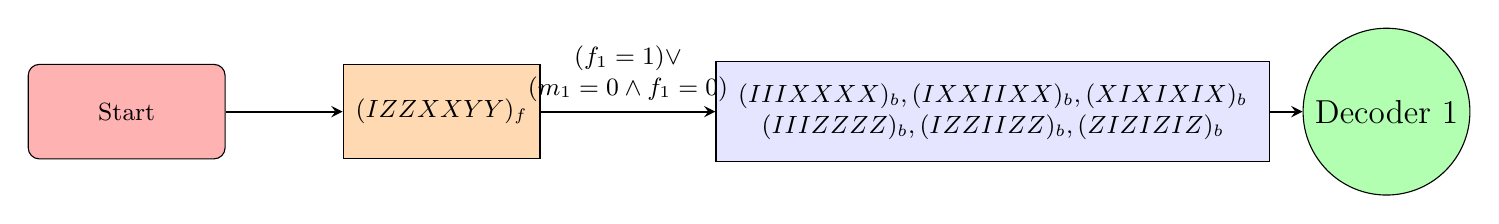
\begin{tikzpicture}[node distance=1.5cm, font=\small] 
        
        % --- 1. Define Styles ---
        \tikzstyle{startstop} = [rectangle, rounded corners, minimum width=2.5cm, minimum height=1.2cm, text centered, draw=black, fill=red!30, font=\small]
        \tikzstyle{raw_syn} = [rectangle, minimum width=2cm, minimum height=1.2cm, inner sep=8pt, text centered, align=center, draw=black, fill=blue!10, font=\small]
        \tikzstyle{flag_syn} = [rectangle, minimum width=2.5cm, minimum height=1.2cm, text centered, align=center, draw=black, fill=orange!30, font=\small]
        \tikzstyle{decode} = [circle, minimum width=2cm, minimum height=1cm, text centered, align=center, draw=black, fill=green!30, font=\large]
        \tikzstyle{arrow} = [thick,->,>=stealth, font=\small]

        % --- 2. Place Nodes ---
        \node (start) [startstop] {Start};
        
        % --- Step 1 ---
        % Increased xshift to space out the nodes and avoid overlap
        \node (pro1) [flag_syn, right of=start, xshift=2.5cm] {$(IZZXXYY)_{f}$};
        
        % Added more xshift here because the stabilizer text is very wide
        \node (pro2b) [raw_syn, right of=pro1, xshift=5.5cm] {$(IIIXXXX)_b, (IXXIIXX)_b, (XIXIXIX)_b$\\$(IIIZZZZ)_b, (IZZIIZZ)_b, (ZIZIZIZ)_b$};
        
        \node (decode1) [decode, right of=pro2b, xshift=3.5cm] {Decoder 1};

        % --- 3. Draw Arrows ---
        \draw [arrow] (start) -- (pro1);
        \draw [arrow] (pro1) -- node[above, align=center] {$ (f_1=1)\vee$\\$(m_1=0 \wedge f_1=0)$} (pro2b);
        \draw [arrow] (pro2b) -- (decode1);
        
    \end{tikzpicture}
    \end{adjustbox}
    \caption{Control flow diagram for the first step of the protocol.} 
    \label{fig:protocol-step-1}
\end{figure}

\begin{figure}[htbp]
    \centering
    % --- First Circuit ---
    \begin{minipage}{0.48\textwidth}
        \centering
        \begin{adjustbox}{max width=\linewidth}
        \begin{quantikz}[row sep=0.25cm, column sep=0.25cm]
            % Data Qubits
            \lstick{$d_1$} & \qw      & \qw      & \qw      & \qw                           & \qw      & \qw                            & \ctrl{8} & \qw      & \qw      & \qw      & \qw      & \qw \\
            \lstick{$d_2$} & \ctrl{6} & \qw      & \qw      & \qw                           & \qw      & \qw                            & \qw      & \qw      & \qw      & \qw      & \qw      & \qw \\
            \lstick{$d_3$} & \qw      & \ctrl{5} & \qw      & \qw                           & \qw      & \qw                            & \qw      & \ctrl{6} & \qw      & \qw      & \qw      & \qw \\
            \lstick{$d_4$} & \qw      & \qw      & \qw      & \qw                           & \qw      & \qw                            & \qw      & \qw      & \qw      & \qw      & \qw      & \qw \\
            \lstick{$d_5$} & \qw      & \qw      & \qw      & \qw                           & \qw      & \qw                            & \qw      & \qw      & \ctrl{4} & \qw      & \qw      & \qw \\
            \lstick{$d_6$} & \qw      & \qw      & \ctrl{2} & \gate[style={fill=red!30}]{Z} & \qw      & \qw                            & \qw      & \qw      & \qw      & \qw      & \qw      & \gate[style={fill=blue!30}]{Z}\\
            \lstick{$d_7$} & \qw      & \qw      & \qw      & \qw                           & \ctrl{1} & \qw                            & \qw      & \qw      & \qw      & \ctrl{2} & \qw      & \gate[style={fill=blue!30}]{Z} \\
            % Ancilla for (IZZIIZZ)
            \lstick{$a_1 \ket{0}$} & \targ{}  & \targ{}  & \targ{}  & \gate[style={fill=red!30}]{Z} & \targ{}  & \qw                            & \qw      & \qw      & \qw      & \qw   &\gate[style={fill=blue!30}]{Z}   & \meter{}  \\
            % Ancilla for (ZIZIZIZ)
            \lstick{$a_2 \ket{0}$} & \qw      & \qw      & \qw      & \qw                           & \qw      & \qw                            & \targ{}  & \targ{}  & \targ{}  & \targ{}  & \qw & \meter{}  
        \end{quantikz}
        \end{adjustbox}
        \caption{First case: A $ZZ$ error (red) caused by a fault on the third CNOT. This propagates to a $ZZ$ error (blue) on the $d_6, d_7$ data qubits and a $Z$ error (blue) on the ancilla $a_1$, which does not alter the measurement outcome.}
        \label{fig:example_2_case_1}
    \end{minipage}\hfill
    % --- Second Circuit ---
    \begin{minipage}{0.48\textwidth}
        \centering
        \begin{adjustbox}{max width=\linewidth}
        \begin{quantikz}[row sep=0.25cm, column sep=0.25cm]
            % Data Qubits
            \lstick{$d_1$} & \qw      & \qw      & \qw      & \qw      & \ctrl{8} &  \gate[style={fill=red!30}]{Z} & \qw      & \qw      & \qw      & \qw      & \gate[style={fill=blue!30}]{Z} \\
            \lstick{$d_2$} & \ctrl{6} & \qw      & \qw      & \qw      & \qw      & \qw      & \qw      & \qw      & \qw      & \qw      & \qw \\
            \lstick{$d_3$} & \qw      & \ctrl{5} & \qw      & \qw      & \qw      & \qw      & \ctrl{6} & \qw      & \qw      & \qw      & \qw \\
            \lstick{$d_4$} & \qw      & \qw      & \qw      & \qw      & \qw      & \qw      & \qw      & \qw      & \qw      & \qw      & \qw \\
            \lstick{$d_5$} & \qw      & \qw      & \qw      & \qw      & \qw      & \qw      & \qw      & \ctrl{4} & \qw      & \qw      & \qw \\
            \lstick{$d_6$} & \qw      & \qw      & \ctrl{2} & \qw      & \qw      & \qw      & \qw      & \qw      & \qw      & \qw      & \qw \\
            \lstick{$d_7$} & \qw      & \qw      & \qw      & \ctrl{1} & \qw      & \qw      & \qw      & \qw      & \ctrl{2} & \qw      & \qw \\
            % Ancilla for (IZZIIZZ)
            \lstick{$a_1 \ket{0}$} & \targ{}  & \targ{}  & \targ{}  & \targ{}  & \qw      & \qw      & \qw      & \qw      & \qw      & \meter{} & \qw \\
            % Ancilla for (ZIZIZIZ)
            \lstick{$a_2 \ket{0}$} & \qw      & \qw      & \qw      & \qw      & \targ{}  & \qw      & \targ{}  & \targ{}  & \targ{}  & \meter{} & \qw 
        \end{quantikz}
        \end{adjustbox}
        \caption{Second case: A $Z$ error (red) caused by a fault on the fifth CNOT. The resulting $Z$ error (blue) propagates to the data qubit.}
        \label{fig:example_2_case_2}
    \end{minipage}
\end{figure}




\section{Conclusion}

In this paper, we presented a formal verification framework for fault-tolerant flagged error correction protocols. 
Rather than explicitly constructing a decoder, we established a necessary and sufficient condition
for FTEC in terms of the residual errors compatible with each measurement record. 
Our SAT-based approach provides a systematic way to verify this
condition and to identify concrete design flaws in flagged protocols.
In particular, it can help detect errors that are difficult to uncover by
manual verification, especially in optimized protocols with reduced circuit
depth, flag-qubit sharing, or adaptive control flow.

In future work, we plan to extend our Pauli-tracking encoding to other
fault-tolerant gadgets and broader quantum computing architectures, such as
measurement-based quantum computation.


% \section*{Data-Availability Statement}
% The artifact consists of a python prototype used to support the results in the paper. The current version is complete but with restricted documentation. We intend to submit this artifact for Artifact Evaluation.





\bibliographystyle{ACM-Reference-Format} 
\bibliography{refs,qecc}



% \clearpage
% \appendix

% \section{Lemma Proof}
% \begin{lemma}
% For a QECC with a stabilizer group $\mathcal{S} = \langle g_1, \dots, g_{n-k} \rangle$ and logical operators $\mathcal{L} = \{\bar{X}_1, \dots, \bar{X}_k, \bar{Z}_1, \dots, \bar{Z}_k\}$, if a Pauli string $P$ commutes with all generators $g_i$ and all logical operators $\bar{X}_j, \bar{Z}_j$, then $P$ lies in the group $\mathcal{S}$ (up to an overall phase).
% \end{lemma}

% \begin{proof}
% The codespace $\mathcal{C}$ stabilized by the group $\mathcal{S}$ is defined as:
% \[
% \mathcal{C} = \{\,|\psi\rangle : G|\psi\rangle = |\psi\rangle \ \forall G \in \mathcal{S}\,\}.
% \]
% Since $P$ commutes with every generator $G_i$, it commutes with all of $\mathcal{S}$. Hence, for any
% $|\psi\rangle \in \mathcal{C}$ and any $G \in \mathcal{S}$,
% \[
% G(P|\psi\rangle) = P(G|\psi\rangle) = P|\psi\rangle,
% \]
% so $P$ maps $\mathcal{C}$ to itself.

% Fix the logical computational basis $\{|z\rangle_L\}_{z\in\{0,1\}^k} \subset \mathcal{C}$
% defined by
% \[
% \bar{Z}_j |z\rangle_L = (-1)^{z_j}|z\rangle_L \qquad (j=1,\dots,k).
% \]
% Because $P$ commutes with every $\bar{Z}_j$, it preserves each joint eigenspace of the
% commuting family $\{\bar{Z}_j\}_{j=1}^k$. In particular, each $|z\rangle_L$ is an eigenvector of
% $P$:
% \[
% P|z\rangle_L = \lambda_z |z\rangle_L
% \]
% for some phase $\lambda_z$ (indeed $\lambda_z \in \{\pm 1, \pm i\}$ since $P \in \mathcal{P}_n$).

% Now use commutation with the logical $\bar{X}_j$. For any $j$ and any bitstring $z$,
% \[
% P(\bar{X}_j|z\rangle_L) = \bar{X}_j(P|z\rangle_L) = \lambda_z\,\bar{X}_j|z\rangle_L.
% \]
% Since $\bar{X}_j|z\rangle_L = |z\oplus e_j\rangle_L$, the left-hand side is also
% \[
% P|z\oplus e_j\rangle_L = \lambda_{z\oplus e_j}|z\oplus e_j\rangle_L,
% \]
% hence
% \[
% \lambda_{z\oplus e_j} = \lambda_z \qquad \forall z,\ \forall j.
% \]
% Because the bit flips $z \mapsto z\oplus e_j$ connect all bitstrings in $\{0,1\}^k$, it follows that
% $\lambda_z$ is independent of $z$; write $\lambda_z=\lambda$ for all $z$. Therefore,
% \[
% P|\psi\rangle = \lambda |\psi\rangle \qquad \forall |\psi\rangle \in \mathcal{C},
% \]
% i.e., $P$ acts as a global phase on the entire codespace.

% Equivalently, the induced logical operator of $P$ is trivial. Hence $P$ represents the
% identity element in the quotient $C(\mathcal{S})/\mathcal{S}$, where $C(\mathcal{S})$ is the centralizer of $\mathcal{S}$. Thus, there exists an element $S' \in \mathcal{S}$ such that
% $P = \lambda S'$. We conclude that $P \in \mathcal{S}$ up to an overall phase, as claimed.
% \end{proof}




% To generate the version WITHOUT the appendix, comment out the line below:
\newpage
\appendix
\section{Proof of Main Theorem}
\label{app:proof}

\begin{theorem}
\label{thm:mains-appendix}
 Consider a flagged error correction protocol $\Pi$ for a stabilizer code
with stabilizer group $\cS$, distance $d$, and
$t=\lfloor (d-1)/2 \rfloor$. Assume that $\Pi$ is valid in the sense of Def.~\ref{def:protocol-validity}
Then there exists a suitable lookup-table decoder $D$ such that $(\Pi,D)$ satisfies
FTEC if and only if, for all measurement record $m$,
$\forall E_1,E_2\in \mathcal{E}_{m},
    E_1\cdot E_2 \notin N(\cS) \setminus \cS$.  
\end{theorem}\label{thm:ftec-verify}

% \begin{theorem}
% \label{thm:mains}
% Consider a flagged error correction protocol for a QECC of distance $d$ and $t = \lfloor\frac{d-1}{2} \rfloor$. Assume that the protocol satisfies Def.~\ref{def:protocol-validity}. 
% The flagged error correction protocol, coupled with any suitable LUT decoder from Definition~\ref{def:decoder}, achieves fault-tolerant error correction if and only if for each $m$, $\forall E_1, E_2 \in \mathcal{E}_{m}$, $E_1 \cdot E_2 \notin \mathcal{N(S)} \setminus \mathcal{S}$.
% \end{theorem}\label{thm:ftec-verify}

\begin{proof}
\textbf{($\Rightarrow$) 
Let $E_1$ and $E_2$ be any two possible residual errors in $\mathcal{E}_{m}$ resulting from distinct fault events. Assume the protocol achieves FTEC. We must show $E_1 \cdot E_2 \notin N(\cS) \setminus \cS$.}\\
We proceed by contradiction. Suppose $E_1 \cdot E_2 \in N(\cS) \setminus \cS$.  This implies that there exists a measurement record $m$ for which the LUT decoder outputs a correction $C$ such that $E_1 \cdot E_2 = (E_1 \cdot C) \cdot (E_2 \cdot C)$ constitutes a logical operator. Suppose that both $\mathrm{wt}_{\mathrm{min}}(E_1 \cdot C)$ and $\mathrm{wt}_{\mathrm{min}}(E_2 \cdot C)$ are at most $t$. Then, their product would have a  $\mathrm{wt}_{\mathrm{min}}$ of at most $2t$. However, because $(E_1 \cdot C) \cdot (E_2 \cdot C)$ is a logical operator, $\mathrm{wt}_{\mathrm{min}}((E_1 \cdot C) \cdot (E_2 \cdot C))$ must be at least $d > 2t$, which yields a contradiction. Therefore, if $\mathrm{wt}_{\mathrm{min}}(E_1 \cdot C) \leq t$, then $\mathrm{wt}_{\mathrm{min}}(E_2 \cdot C)>t$ , and vice versa. It follows that either $(E_1 \cdot C)$ or $(E_2 \cdot C)$ must violate FTEC (2) of Def.~\ref{def:weak-FTEC}.

\textbf{($\Leftarrow$) 
Assume $\forall E_1 , E_2 \in \mathcal{E}_m,  E_1 \cdot E_2 \notin  N(\cS) \setminus \cS$. We must show the protocol achieves FTEC.}
\paragraph{Termination Condition (1).}
Let $m$ be the corresponding
    measurement record, and let $C\in\mathcal{E}_m$ be the representative
    correction chosen by the LUT decoder.
    Since all residual errors in $\mathcal{E}_m$ have the same ideal syndrome,
    for every $E\in\mathcal{E}_m$,
    $\operatorname{syn}(E)=\operatorname{syn}(C)$.
    Hence, $\operatorname{syn}(E\cdot C)=0,$ which implies $E\cdot C\in N(\mathcal{S}).$
    On the other hand, both $E$ and $C$ belong to $\mathcal{E}_m$. By the
    assumption of the theorem, $E \cdot C \notin N(\mathcal{S}) \setminus \mathcal{S}$. 
    Therefore, $E \cdot C\in S$.
    Thus, after applying the representative correction, every possible residual
    error is equivalent to the identity up to a stabilizer. Hence the logical
    state is preserved, and FTEC of Definition~\ref{def:weak-FTEC} is satisfied.
        
\paragraph{Termination Condition (2).}
Let $w$ be the number of faults detected
before the final repeated full-syndrome suffix.  By Condition~(2), this suffix
consists of $t-w+1$ consecutive full syndrome extraction rounds whose measured
syndrome outcomes are all equal to the same value $\sigma$, and no flag is
raised during these rounds.

Fix an execution with total fault number $s\le t$.  Since at least $w$ faults
have already been detected before the suffix, at most $s-w\le t-w$ faults occur
during the repeated full-syndrome suffix.  Hence, among the $t-w+1$ full
syndrome extraction rounds in the suffix, at least one round is fault-free.
Fix such a fault-free round $R$, and let $E^-$ be the data error immediately
before $R$.
Because $R$ is fault-free and the full syndrome extraction circuit is correct,
the measured syndrome outcome of $R$ is exactly the ideal syndrome of $E^-$.
Since all rounds in the repeated suffix report the same syndrome value
$\sigma$, we have
$\operatorname{syn}(E^-)=\sigma$.
Moreover, by correctness of the fault-free syndrome extraction circuit, $R$
introduces no additional data error, so the data error immediately after $R$ is
still $E^-$.

Now consider
another execution that has the same faults as the original execution up to $R$,
but has no faults after $R$.  Since $R$ is fault-free and the later full
syndrome extraction rounds are also fault-free in this execution, the data
error remains $E^-$ throughout the rest of the suffix.  Moreover, all later
rounds report the same syndrome value $\sigma$ and raise no flag.  Hence this
execution follows the same terminating path, has the same measurement record
$m$, and has final residual data error $E^-$.  Therefore $E^-\in\mathcal E_m$.
Thus all possible errors $E^-$ arising immediately before a fault-free round
in the repeated suffix are equivalent up to stabilizers.  For the record $m$,
choose the decoder output $C$ to be one representative of this equivalence
class.  Then, for the prefix error $E^-$ in the actual execution,
$C\cdot E^- \in \mathcal S$. This does not yet account for faults occurring after $R$; these faults are
handled separately below.
Let $E_{\mathrm{suf}}$ denote the data error induced by faults occurring after
$R$ in the repeated full-syndrome suffix.  By Pauli propagation through Clifford
circuits, the final data error before applying the decoder output can be written,
up to global phase, as
$E_{\mathrm{fin}} = E^- \cdot E_{\mathrm{suf}}$.
Therefore, after applying the decoder output $C$, $C\cdot E_{\mathrm{fin}}
    =
    C\cdot E^- E_{\mathrm{suf}}
    \sim
    E_{\mathrm{suf}}$, because $C\cdot E^-\in\mathcal S$.

It remains to bound $E_{\mathrm{suf}}$. The number of faults occurring after
$R$ is at most $s-w$. Since no flag is raised during the repeated suffix and the
full syndrome extraction circuit satisfies the required $(t-w)$-flag condition,
these faults induce a data error satisfying
$\mathrm{wt}_{\min}(E_{\mathrm{suf}})\le s-w\le s$.
Hence
$\mathrm{wt}_{\min}(C\cdot E_{\mathrm{fin}})
    =
    \mathrm{wt}_{\min}(E_{\mathrm{suf}})
    \le s$.
This proves FTEC~(2) of Def.~\ref{def:weak-FTEC}.

For FTEC (1), observe that the error accumulated before $R$ is canceled
up to stabilizer equivalence by the decoder output, since $C\cdot E^-\in\mathcal S$.
Thus the output data block differs from the ideally decoded input only by the
suffix error $E_{\mathrm{suf}}$, up to stabilizer equivalence. Since
$\mathrm{wt}_{\min}(E_{\mathrm{suf}})\le s\le t$, ideal decoding removes this
remaining error. Therefore, ideal decoding of the output data block gives the
same logical state as ideal decoding of the input data block. This proves
FTEC~(1) of Def.~\ref{def:weak-FTEC}.

\paragraph{Termination Condition (3).}
\yfc{Please check whether this argument establishes the required
residual-weight bound $s$ for $r+s\le t$, rather than only a bound of $t$.}
For any fault event of weight $w \leq t$, every resulting error $E \in \mathcal{E}_m$ has a  weight $\mathrm{wt}_{\min}(E) \leq t$, thereby satisfying FTEC (2) of Def~\ref{def:weak-FTEC}. Consequently, applying an ideal decoder to an input state---which contains an initial data error of weight $r \leq t$ and an accumulated output error $E$ with $\mathrm{wt}_{\min}(E) \leq t$---will successfully recover the original state. This holds because, for any quantum error-correcting code with distance $d$, every error $e$ with $\mathrm{wt}_{\min}(e) \leq t$ is perfectly correctable via ideal decoding, thus satisfying FTEC (1) of Def~\ref{def:weak-FTEC}.


\end{proof}

\section{section 3 appendix}
\yfc{Please replace this placeholder appendix title with a descriptive title.}
\yfc{Please recompile the PDF after the restructuring and check for
undefined references, multiply defined labels, and figure placement.}
\begin{theorem}
\label{thm:syndrome-extraction-valid}
\yfc{This label is also used by the theorem in the main text.
Please give the appendix restatement a distinct label and check
that all references point to the intended theorem.}
Let $U$ be a Clifford syndrome extraction circuit
before the final ancilla measurements. Let
\[
    \mathcal{S}_{\mathrm{data}}
    =\langle G_1,\ldots,G_{n-k}\rangle,
    \qquad
    \mathcal{S}_{\mathrm{anc}}
    =\langle A_1,\ldots,A_r\rangle
\]
be the data stabilizer group and the stabilizer group
of the prepared ancillas, respectively, where each
$A_i$ is the corresponding single-qubit preparation
and measurement observable.

Among the $r$ ancillas, the first $m$ are designated
for extracting the Pauli checks
$\{P_i\}_{i=1}^{m}\subseteq\mathcal{S}_{\mathrm{data}}$,
where $m\leq r$.

Define
\[
    \mathcal{S}_{\mathrm{joint}}
    =\langle G_1,\ldots,G_{n-k},
               A_1,\ldots,A_r\rangle.
\]
Let $L_1,\ldots,L_{2k}$ be Hermitian representatives
of a complete set of logical Pauli generators.
Identity extensions on the complementary register
are understood.

Then $U$ is valid if and only if $U$ is correct
and the following conditions hold:
\[
\begin{gathered}
    \mathcal{S}'_{\mathrm{joint}}
    =U\mathcal{S}_{\mathrm{joint}}U^\dagger
    =\mathcal{S}_{\mathrm{joint}},
    \\
    (UL_iU^\dagger)L_i\in\mathcal{S}_{\mathrm{joint}}
    \qquad\text{for every }i=1,\ldots,2k.
\end{gathered}
\]
Both stabilizer equality and membership retain
the Pauli signs.
\end{theorem}

\begin{proof}
\label{app:proof-syndrome-extraction}
\textbf{($\Leftarrow$).}
Suppose $U$ is correct and both preservation
conditions hold.

Joint stabilizer preservation implies that $U$
maps the joint stabilized subspace onto itself.
Moreover, logical preservation implies that
\[
    UL_iU^\dagger=L_iS_i
\]
for some $S_i\in\mathcal{S}_{\mathrm{joint}}$.
Since every $S_i$ acts as the identity on the
joint stabilized subspace, the restriction of
$U$ to this subspace commutes with every logical
Pauli generator.

As the logical Pauli generators act irreducibly
on the encoded logical space, $U$ acts as a
common global phase on the entire joint
stabilized subspace. Thus, for every codespace
state $\ket{\psi}$ and prepared ancilla state
$\ket{a}$,
\[
    U(\ket{\psi}\otimes\ket{a})
    =e^{i\theta}\ket{\psi}\otimes\ket{a}.
\]

For an arbitrary input Pauli error $E$,
Clifford propagation gives
\[
    U(E\otimes I_{\mathrm{anc}})U^\dagger
    =\omega(E'\otimes E_{\mathrm{anc}}).
\]
Consequently,
\[
    U(E\ket{\psi}\otimes\ket{a})
    =\omega e^{i\theta}
      E'\ket{\psi}\otimes
      E_{\mathrm{anc}}\ket{a}.
\]
Since $E_{\mathrm{anc}}$ is a Pauli operator,
each ancilla measurement outcome is uniquely
determined by the commutation parity
$E_{\mathrm{anc}}\odot A_i$, independently
of the encoded state.
Furthermore, correctness guarantees
$E'\sim E$, so the output data remains in
the codespace up to a Pauli error.

For $E=I$, all ancilla outcomes are $+1$
and the encoded logical state is unchanged.
Hence $U$ is deterministic and therefore valid.

\textbf{($\Rightarrow$).}
Suppose $U$ is valid, and hence correct and
deterministic.

Let $\ket{a}$ be the prepared ancilla state.
For $E=I$, determinism requires all ancilla
outcomes to be $+1$ and the encoded logical
state to remain unchanged.
Since the joint $+1$ eigenspace of the ancilla
measurement observables is one-dimensional,
the premeasurement state must satisfy
\[
    U(\ket{\psi}\otimes\ket{a})
    =e^{i\theta}\ket{\psi}\otimes\ket{a}
\]
for every codespace state $\ket{\psi}$,
with a common phase by linearity.

Thus $U$ acts as a global phase on the entire
joint stabilized subspace. In particular,
conjugation by $U$ preserves its signed Pauli
stabilizer group. Since $U$ is Clifford,
\[
    \mathcal{S}'_{\mathrm{joint}}
    =U\mathcal{S}_{\mathrm{joint}}U^\dagger
    =\mathcal{S}_{\mathrm{joint}}.
\]

Moreover, each logical Pauli generator $L_i$
preserves the joint stabilized subspace and
satisfies $L_i^2=I$. Therefore,
\[
    (UL_iU^\dagger)L_i
    (\ket{\psi}\otimes\ket{a})
    =\ket{\psi}\otimes\ket{a}
\]
for every codespace state $\ket{\psi}$.

Since $U$ is Clifford, the operator
$(UL_iU^\dagger)L_i$ is a Pauli operator.
It acts as the identity on the entire joint
stabilized subspace and therefore belongs to
its signed Pauli stabilizer group:
\[
    (UL_iU^\dagger)L_i
    \in\mathcal{S}_{\mathrm{joint}}.
\]
Hence both preservation conditions hold.
\end{proof}


% ==========================================
% TABLE: Stabilizer Evolution
% ==========================================
\begin{table}[h]
    \centering
    \renewcommand{\arraystretch}{1.5}
    \begin{tabular}{|c|c|c|c|c|}
        \hline
        \textbf{Initial Operator} & \textbf{CNOT$_{Q_{anc1}, Q_1}$} & \textbf{CNOT$_{Q_2, Q_{anc2}}$} & \textbf{CNOT$_{Q_{anc1}, Q_2}$} & \textbf{CNOT$_{Q_1, Q_{anc2}}$} \\
        \hline
        $X_{Q_1} X_{Q_2} I_{anc1} I_{anc2}$ & $X_{Q_1} X_{Q_2} I_{anc1} I_{anc2}$ & $X_{Q_1} X_{Q_2} I_{anc1} X_{anc2}$ & $X_{Q_1} X_{Q_2} I_{anc1} X_{anc2}$ & \textbf{$X_{Q_1} X_{Q_2} I_{anc1} I_{anc2}$} \\
        \hline
        $Z_{Q_1} Z_{Q_2} I_{anc1} I_{anc2}$ & $Z_{Q_1} Z_{Q_2} Z_{anc1} I_{anc2}$ & $Z_{Q_1} Z_{Q_2} Z_{anc1} I_{anc2}$ & $Z_{Q_1} Z_{Q_2} I_{anc1} I_{anc2}$ & \textbf{$Z_{Q_1} Z_{Q_2} I_{anc1} I_{anc2}$} \\
        \hline
        $I_{Q_1} I_{Q_2} X_{anc1} I_{anc2}$ & $X_{Q_1} I_{Q_2} X_{anc1} I_{anc2}$ & $X_{Q_1} I_{Q_2} X_{anc1} I_{anc2}$ & $X_{Q_1} X_{Q_2} X_{anc1} I_{anc2}$ & \textbf{$X_{Q_1} X_{Q_2} X_{anc1} X_{anc2}$} \\
        \hline
        $I_{Q_1} I_{Q_2} I_{anc1} Z_{anc2}$ & $I_{Q_1} I_{Q_2} I_{anc1} Z_{anc2}$ & $I_{Q_1} Z_{Q_2} I_{anc1} Z_{anc2}$ & $I_{Q_1} Z_{Q_2} Z_{anc1} Z_{anc2}$ & \textbf{$Z_{Q_1} Z_{Q_2} Z_{anc1} Z_{anc2}$} \\
        \hline
    \end{tabular}
    % \caption{$\mathcal{S}_{data}=\langle X_{Q1}X_{Q2}, Z_{Q_1}Z_{Q_2} \rangle$ and $\mathcal{S}_{anc} = \langle X_{anc1}I_{anc2} ,  I_{anc1}Z_{ancX} \rangle$. The table is the evolution of stabilizer generator of $\mathcal{S}_{joint}$. It can verify that the pauli string$I_{Q_1} I_{Q_2} X_{anc1} I_{anc2}$and  $I_{Q_1} I_{Q_2} I_{anc1} Z_{anc2}$ does not commute with all the Pauli string after evolution hence the measurement outcomes on ancillas are not deterministic.}
    \caption{This table tracks the stabilizer evolution of a joint data-ancilla system initialized with $\mathcal{S}_{\mathrm{data}}=\langle X_{Q_1}X_{Q_2}, Z_{Q_1}Z_{Q_2}\rangle$ and $\mathcal{S}_{\mathrm{anc}}=\langle X_{\mathrm{anc1}}I_{\mathrm{anc2}}, I_{\mathrm{anc1}}Z_{\mathrm{anc2}}\rangle$ through a parallel syndrome extraction circuit. After the circuit's execution, we can verify that the evolved group $\mathcal{S}'_{\mathrm{joint}}$ is not identical to the initial group $\mathcal{S}_{\mathrm{joint}}$, thereby violating Definition~\ref{def:syndrome-extraction-deterministic}. Furthermore, the emergence of the operators $X_{\mathrm{anc1}}X_{\mathrm{anc2}}$ and $Z_{\mathrm{anc1}}Z_{\mathrm{anc2}}$ in the final stabilizer group indicates that the two ancilla qubits have formed a maximally entangled state. Consequently, their individual measurement outcomes are no longer deterministic.}
    \label{tab:stabilizer-evolution}
\end{table}


\end{document}

